\chapter{Deep network training and regularization}
\label{sec:deep_network_training_and_regularization}

In Chapters~\ref{sec:deep_feedforward_and_backpropagation} and~\ref{sec:convolutional_neural_networks}, we developed the architectural foundations of deep learning: Multilayer Perceptrons capable of universal function approximation and Convolutional Neural Networks endowed with an infinitely strong spatial prior. In theory, once a loss function $\mathcal{L}$ and a computational graph are defined, the Backpropagation algorithm evaluates exact parameter gradients $\nabla_{\boldsymbol{\theta}} \mathcal{L}$, and first-order optimizers (such as Stochastic Gradient Descent or Adam, derived in Chapter~\ref{sec:linear_predictors_and_gradient_optimization}) iteratively minimize empirical risk.

In practice, however, when researchers in the early 2000s attempted to train feedforward or convolutional networks with more than a few hidden layers, \textbf{naive training catastrophically broke down}:
\begin{enumerate}[noitemsep,topsep=2pt,parsep=0pt,partopsep=0pt]
  \item \textbf{Gradient vanishing and explosion}: Propagating signals across dozens of cascading layers caused gradients to decay exponentially toward zero or explode toward numerical overflow, halting learning in early layers.
  \item \textbf{Activation pathologies and the dying neuron trap}: Classical activations saturated, while ReLUs suffered from catastrophic deactivation, permanently extinguishing large percentages of the network.
  \item \textbf{Initialization sensitivity}: Initializing weights with values that were slightly too small caused activation variances to collapse to zero; initializing weights slightly too large drove activations into saturated regimes.
  \item \textbf{Internal covariate shift}: Continuous parameter updates in early layers altered the distribution of inputs feeding downstream layers, forcing subsequent layers to constantly chase a moving target distribution.
  \item \textbf{Overfitting in overparameterized regimes}: Deep architectures possessing millions of parameters easily memorized noise and training idiosyncrasies, leading to massive generalization gaps.
\end{enumerate}

To transform deep neural networks from unstable mathematical curiosities into robust, scalable engineering systems, machine learning had to conquer the \textbf{numerical physics of deep training}. This chapter investigates the theoretical breakthroughs that unlocked deep network optimization: from activation function dynamics and data preprocessing, through Xavier and He weight initialization theory, to Batch Normalization and modern regularization paradigms.

\section{Activation dynamics and pathologies}
\label{sec:activation_dynamics_pathologies}

Before analyzing the specific failure modes of deep neural network optimization, we must establish why \textbf{activation functions} constitute the foundational engine of representation learning, and why their numerical behavior fundamentally dictates whether a deep architecture can be trained.

\paragraph{The Linear Collapse Theorem:}
Consider a feedforward network with $L$ hidden layers, weight matrices $\mathbf{W}^{(l)} \in \R^{d_l \times d_{l-1}}$, and bias vectors $\mathbf{b}^{(l)} \in \R^{d_l}$. Suppose we omit the nonlinear activation functions, computing layer activations purely as linear transformations:
\begin{equation}
\mathbf{a}^{(l)} = \mathbf{z}^{(l)} = \mathbf{W}^{(l)} \mathbf{a}^{(l-1)} + \mathbf{b}^{(l)}, \quad \text{for } l = 1, \dots, L, \quad \text{with } \mathbf{a}^{(0)} = \vx.
\end{equation}
Unrolling this composition from the output layer $\hat{\vy} = \mathbf{a}^{(L)}$ back to the input $\vx$ yields:
\begin{align}
\hat{\vy} &= \mathbf{W}^{(L)} \left( \mathbf{W}^{(L-1)} \left( \cdots \left( \mathbf{W}^{(1)} \vx + \mathbf{b}^{(1)} \right) \cdots \right) + \mathbf{b}^{(L-1)} \right) + \mathbf{b}^{(L)} \notag \\
&= \left( \prod_{l=1}^L \mathbf{W}^{(l)} \right) \vx + \sum_{k=1}^{L-1} \left( \prod_{m=k+1}^L \mathbf{W}^{(m)} \right) \mathbf{b}^{(k)} + \mathbf{b}^{(L)}.
\label{eq:linear_collapse_derivation}
\end{align}
Because matrix multiplication is associative and the space of linear transformations is closed under composition, the product of $L$ weight matrices collapses into a single effective matrix $\mathbf{W}_{\text{eff}} \triangleq \prod_{l=1}^L \mathbf{W}^{(l)} \in \R^{d_L \times d_0}$, while the accumulated affine shifts collapse into a single effective bias vector $\mathbf{b}_{\text{eff}} \in \R^{d_L}$. Therefore:
\begin{equation}
\hat{\vy} = \mathbf{W}_{\text{eff}} \vx + \mathbf{b}_{\text{eff}}.
\label{eq:linear_collapse}
\end{equation}
Equation~\eqref{eq:linear_collapse} establishes an inescapable theoretical result: \textbf{any purely linear neural network, regardless of its depth, parameter count, or number of layers, is mathematically identical to a single-layer linear model}. It cannot compute the simple XOR function, cannot represent non-convex decision boundaries, and possesses zero hierarchical feature abstraction capacity.

\paragraph{Universal Approximation and the Non-Linear Engine:}
By the Universal Approximation Theorem~\cite{cybenko1989approximation,hornik1989multilayer}, introducing a continuous, non-polynomial activation function $\sigma: \R \to \R$ after each affine transformation:
\begin{equation}
\mathbf{a}^{(l)} = \sigma(\mathbf{z}^{(l)}) = \sigma\left(\mathbf{W}^{(l)} \mathbf{a}^{(l-1)} + \mathbf{b}^{(l)}\right)
\end{equation}
endows the network with the mathematical expressivity to approximate any continuous function on compact subsets of $\R^d$ to arbitrary precision. The activation function is the sole architectural mechanism responsible for bending, folding, and untangling the geometric manifold of the data.

\paragraph{The Numerical Dilemma of Non-Linearity:}
However, the activation function is a double-edged sword. While it introduces the non-linearity required for expressive capacity on the forward pass, its \textbf{local first derivative} $\sigma'(z)$ acts as a scalar multiplicative gate during the backward pass via the chain rule of calculus. 
If $\sigma'(z)$ is poorly conditioned, training a deep network encounters severe numerical instabilities:
\begin{enumerate}[noitemsep,topsep=2pt,parsep=0pt,partopsep=0pt]
  \item \textbf{Vanishing Gradients}: If the derivative satisfies $|\sigma'(z)| < 1$, multiplying derivatives across $L$ layers causes the gradient to decay exponentially toward zero, starving early layers of learning signals.
  \item \textbf{Exploding Gradients}: If derivatives and weight spectral norms combine such that the effective transition multiplier exceeds 1, gradients grow exponentially, causing numerical overflow and parameter divergence.
  \item \textbf{Optimization Zigzagging}: If $\sigma(z)$ is strictly non-zero centered (e.g., $\sigma(z) > 0$), all weight gradients entering a neuron share identical signs, restricting parameter updates to two opposite orthants and forcing the optimizer into slow zigzagging trajectories.
  \item \textbf{Dead Neurons}: If $\sigma(z)$ contains a flat, inactive region with zero derivative ($\sigma'(z) = 0$), large gradient steps can push neurons into permanent comas where gradients vanish across the entire dataset.
  \item \textbf{Computational Inefficiency}: Activation functions involving transcendental functions ($\exp, \log$) incur significant computational latency on hardware accelerators compared to simple thresholding comparators.
\end{enumerate}
Understanding these five interconnected phenomena is essential to mastering modern deep network optimization.

\subsection{Vanishing and exploding gradients}
\label{sec:vanishing_exploding_gradients}

To understand why deep networks fail to train out of the box, we analyze the analytical structure of backpropagation across an $L$-layer network from first principles.

\paragraph{Derivation of the Layer Error Recurrence (Formula 6.1):}
Consider an $L$-layer feedforward network defined by the forward recurrence:
\begin{equation}
\mathbf{z}^{(l)} = \mathbf{W}^{(l)} \mathbf{a}^{(l-1)} + \mathbf{b}^{(l)}, \qquad \mathbf{a}^{(l)} = \sigma(\mathbf{z}^{(l)}),
\end{equation}
where $\mathbf{W}^{(l)} \in \R^{d_l \times d_{l-1}}$, $\mathbf{b}^{(l)} \in \R^{d_l}$, and $\sigma(\cdot)$ is applied element-wise. Let $\mathcal{L}$ denote the scalar training loss. We define the error adjoint vector at layer $l$ as the gradient of the loss with respect to pre-activation vector $\mathbf{z}^{(l)}$:
\begin{equation}
\boldsymbol{\delta}^{(l)} \triangleq \frac{\partial \mathcal{L}}{\partial \mathbf{z}^{(l)}} = \begin{bmatrix} \frac{\partial \mathcal{L}}{\partial z_1^{(l)}} & \frac{\partial \mathcal{L}}{\partial z_2^{(l)}} & \cdots & \frac{\partial \mathcal{L}}{\partial z_{d_l}^{(l)}} \end{bmatrix}^\top \in \R^{d_l}.
\end{equation}
To evaluate the $i$-th component $\delta_i^{(l)} = \frac{\partial \mathcal{L}}{\partial z_i^{(l)}}$, we apply the multivariate chain rule across all $d_{l+1}$ units of the subsequent layer $l+1$:
\begin{equation}
\delta_i^{(l)} = \frac{\partial \mathcal{L}}{\partial z_i^{(l)}} = \sum_{j=1}^{d_{l+1}} \frac{\partial \mathcal{L}}{\partial z_j^{(l+1)}} \frac{\partial z_j^{(l+1)}}{\partial a_i^{(l)}} \frac{\partial a_i^{(l)}}{\partial z_i^{(l)}}.
\label{eq:chain_rule_expansion}
\end{equation}
Evaluating each partial derivative component individually:
\begin{itemize}[noitemsep,topsep=2pt,parsep=0pt,partopsep=0pt]
  \item By definition, $\frac{\partial \mathcal{L}}{\partial z_j^{(l+1)}} = \delta_j^{(l+1)}$.
  \item Because $z_j^{(l+1)} = \sum_{k=1}^{d_l} W_{jk}^{(l+1)} a_k^{(l)} + b_j^{(l+1)}$, the partial derivative with respect to activation $a_i^{(l)}$ is:
    \begin{equation}
    \frac{\partial z_j^{(l+1)}}{\partial a_i^{(l)}} = W_{ji}^{(l+1)}.
    \end{equation}
  \item Because $a_i^{(l)} = \sigma(z_i^{(l)})$, the derivative of the element-wise activation with respect to its pre-activation is:
    \begin{equation}
    \frac{\partial a_i^{(l)}}{\partial z_i^{(l)}} = \sigma'(z_i^{(l)}).
    \end{equation}
\end{itemize}
Substituting these three terms back into Equation~\eqref{eq:chain_rule_expansion}:
\begin{equation}
\delta_i^{(l)} = \sum_{j=1}^{d_{l+1}} \delta_j^{(l+1)} W_{ji}^{(l+1)} \sigma'(z_i^{(l)}) = \left( \sum_{j=1}^{d_{l+1}} W_{ji}^{(l+1)} \delta_j^{(l+1)} \right) \sigma'(z_i^{(l)}).
\end{equation}
Recognizing that the summation $\sum_{j=1}^{d_{l+1}} W_{ji}^{(l+1)} \delta_j^{(l+1)}$ represents the $i$-th element of the matrix-vector product $(\mathbf{W}^{(l+1)})^\top \boldsymbol{\delta}^{(l+1)}$, we express this in compact vector notation:
\begin{equation}
\boldsymbol{\delta}^{(l)} = \left( (\mathbf{W}^{(l+1)})^\top \boldsymbol{\delta}^{(l+1)} \right) \odot \sigma'(\mathbf{z}^{(l)}),
\label{eq:recurrence_review}
\end{equation}
where $\odot$ denotes the Hadamard (element-wise) product, and $\sigma'(\mathbf{z}^{(l)}) \in \R^{d_l}$ is the vector of element-wise activation derivatives. This establishes Formula 6.1.

\paragraph{Derivation of the Unrolled Gradient Chain (Formula 6.2):}
To analyze how this error propagates backwards across many layers, we convert the element-wise Hadamard product into matrix multiplication. Notice that for any vector $\mathbf{u} \in \R^d$, $\mathbf{u} \odot \sigma'(\mathbf{z}^{(l)}) = \operatorname{diag}\left(\sigma'(\mathbf{z}^{(l)})\right) \mathbf{u}$, where $\operatorname{diag}\left(\sigma'(\mathbf{z}^{(l)})\right) \in \R^{d_l \times d_l}$ is a diagonal matrix containing the local activation derivatives along its main diagonal:
\begin{equation}
\operatorname{diag}\left(\sigma'(\mathbf{z}^{(l)})\right) = \begin{bmatrix}
\sigma'(z_1^{(l)}) & 0 & \cdots & 0 \\
0 & \sigma'(z_2^{(l)}) & \cdots & 0 \\
\vdots & \vdots & \ddots & \vdots \\
0 & 0 & \cdots & \sigma'(z_{d_l}^{(l)})
\end{bmatrix}.
\end{equation}
Equation~\eqref{eq:recurrence_review} can therefore be written strictly as linear algebraic transformations:
\begin{equation}
\boldsymbol{\delta}^{(l)} = \operatorname{diag}\left(\sigma'(\mathbf{z}^{(l)})\right) (\mathbf{W}^{(l+1)})^\top \boldsymbol{\delta}^{(l+1)}.
\end{equation}
Defining the layer transition Jacobian matrix $\mathbf{J}_k \in \R^{d_k \times d_{k+1}}$ from layer $k+1$ to layer $k$:
\begin{equation}
\mathbf{J}_k \triangleq \operatorname{diag}\left(\sigma'(\mathbf{z}^{(k)})\right) (\mathbf{W}^{(k+1)})^\top \quad \text{or equivalently} \quad (\mathbf{W}^{(k+1)})^\top \operatorname{diag}\left(\sigma'(\mathbf{z}^{(k+1)})\right),
\end{equation}
we unroll the recurrence recursively from output layer $L$ down to early layer $l$:
\begin{align}
\boldsymbol{\delta}^{(L-1)} &= \mathbf{J}_{L-1} \boldsymbol{\delta}^{(L)}, \notag \\
\boldsymbol{\delta}^{(L-2)} &= \mathbf{J}_{L-2} \boldsymbol{\delta}^{(L-1)} = \mathbf{J}_{L-2} \mathbf{J}_{L-1} \boldsymbol{\delta}^{(L)}, \notag \\
\boldsymbol{\delta}^{(l)} &= \mathbf{J}_l \mathbf{J}_{l+1} \cdots \mathbf{J}_{L-1} \boldsymbol{\delta}^{(L)} = \left[ \prod_{k=l}^{L-1} \mathbf{J}_k \right] \boldsymbol{\delta}^{(L)}.
\end{align}
Expanding each Jacobian $\mathbf{J}_k$ explicitly yields Formula 6.2:
\begin{equation}
\boldsymbol{\delta}^{(l)} = \left[ \prod_{k=l}^{L-1} (\mathbf{W}^{(k+1)})^\top \operatorname{diag}\left( \sigma'(\mathbf{z}^{(k)}) \right) \right] \boldsymbol{\delta}^{(L)}.
\label{eq:unrolled_gradient_product}
\end{equation}
Equation~\eqref{eq:unrolled_gradient_product} proves that the error signal $\boldsymbol{\delta}^{(l)}$ reaching any early layer $l$ is a \textbf{repeated product of $L-l$ transition matrices}.

\paragraph{Derivation of the Spectral Bound (Formula 6.3):}
We now bound the magnitude of $\boldsymbol{\delta}^{(l)}$ using the sub-multiplicative property of induced matrix operator norms. Recall that for any matrix $\mathbf{A} \in \R^{m \times n}$ and vector $\mathbf{x} \in \R^n$, the induced Euclidean operator norm (spectral norm, equal to the largest singular value $\sigma_{\max}(\mathbf{A})$) satisfies:
\begin{equation}
\|\mathbf{A} \mathbf{x}\|_2 \le \|\mathbf{A}\|_2 \|\mathbf{x}\|_2, \qquad \|\mathbf{A} \mathbf{B}\|_2 \le \|\mathbf{A}\|_2 \|\mathbf{B}\|_2.
\end{equation}
Taking the Euclidean norm of both sides of Equation~\eqref{eq:unrolled_gradient_product}:
\begin{equation}
\|\boldsymbol{\delta}^{(l)}\|_2 = \left\| \left( \prod_{k=l}^{L-1} \mathbf{J}_k \right) \boldsymbol{\delta}^{(L)} \right\|_2 \le \left( \prod_{k=l}^{L-1} \|\mathbf{J}_k\|_2 \right) \|\boldsymbol{\delta}^{(L)}\|_2.
\end{equation}
Furthermore, by the sub-multiplicative norm property, the norm of each transition Jacobian decomposes into the product of the weight matrix norm and the derivative matrix norm:
\begin{equation}
\|\mathbf{J}_k\|_2 \le \|(\mathbf{W}^{(k+1)})^\top\|_2 \|\operatorname{diag}\left(\sigma'(\mathbf{z}^{(k)})\right)\|_2 = \|\mathbf{W}^{(k+1)}\|_2 \max_{i \in \{1, \dots, d_k\}} \left| \sigma'(z_i^{(k)}) \right|.
\label{eq:jacobian_norm_decomposition}
\end{equation}
Let $\gamma \triangleq \max_{k \in \{l, \dots, L-1\}} \|\mathbf{J}_k\|_2$ denote the upper bound on the layer spectral norm. Applying this upper bound across all $L-l$ transitions yields Formula 6.3:
\begin{equation}
\|\boldsymbol{\delta}^{(l)}\|_2 \le \left( \prod_{k=l}^{L-1} \|\mathbf{J}_k\|_2 \right) \|\boldsymbol{\delta}^{(L)}\|_2 \le \gamma^{L-l} \|\boldsymbol{\delta}^{(L)}\|_2.
\label{eq:spectral_norm_bound}
\end{equation}

\paragraph{The Asymptotic Dichotomy: Vanishing vs. Exploding Gradients:}
Equation~\eqref{eq:spectral_norm_bound} provides the fundamental mathematical explanation for the fragility of deep networks:
\begin{itemize}[leftmargin=*]
  \item \textbf{Vanishing Gradients ($\gamma < 1$)}: If the effective spectral norm $\gamma < 1$, the gradient magnitude decays exponentially with depth: $\|\boldsymbol{\delta}^{(l)}\|_2 \le \gamma^{L-l} \|\boldsymbol{\delta}^{(L)}\|_2 \to 0$. In a network with $L = 50$ layers, if $\gamma \approx 0.8$, the gradient at the first layer is attenuated by $0.8^{50} \approx 1.4 \times 10^{-5}$; if $\gamma \approx 0.25$ (the maximum derivative of Sigmoid), the attenuation is $(0.25)^{50} \approx 7.8 \times 10^{-31}$! Early layers receive virtually zero gradient updates, leaving their weights frozen at their initial random values. Because early layers extract essential low-level primitives (such as edges and textures), freezing them prevents all downstream layers from forming meaningful representations.
  \item \textbf{Exploding Gradients ($\gamma > 1$)}: If $\gamma > 1$, the product grows exponentially: $\|\boldsymbol{\delta}^{(l)}\|_2 \sim \mathcal{O}(\gamma^{L-l}) \to \infty$. A gradient step $\Delta \mathbf{W} = -\eta \nabla_{\mathbf{W}} \mathcal{L}$ takes massive, erratic jumps across the loss surface, catapulting parameters into unstable regions and producing floating-point overflow (\texttt{NaN} or \texttt{Inf}).
\end{itemize}

\subsection{Pathologies of Sigmoid and Tanh}
\label{sec:sigmoid_tanh_pathologies}

For decades, the default non-linearities in neural computation were the smooth sigmoidal functions: the logistic sigmoid $\sigma(z) = \frac{1}{1 + e^{-z}}$ and hyperbolic tangent $\tanh(z) = \frac{e^z - e^{-z}}{e^z + e^{-z}}$. When deployed in deep architectures, both functions induce severe mathematical pathologies that prevent gradient-based learning from scaling beyond a few layers.

\paragraph{1. Saturation and Gradient Vanishing in Sigmoid.}~\cite{glorot2010understanding}
The derivative of the logistic sigmoid is:
\begin{equation}
\sigma'(z) = \sigma(z)(1 - \sigma(z)).
\label{eq:sigmoid_derivative}
\end{equation}
Because $\sigma(z) \in (0, 1)$, we can find the maximum value of $\sigma'(z)$ by differentiating with respect to $z$ and setting to zero: $\sigma''(z) = \sigma'(z)(1 - 2\sigma(z)) = 0$, yielding $\sigma(z^*) = 0.5 \implies z^* = 0$. At this optimum:
\begin{equation}
\max_{z \in \R} \sigma'(z) = \sigma'(0) = 0.5 \times (1 - 0.5) = 0.25.
\label{eq:sigmoid_max_deriv}
\end{equation}
This property is devastating when evaluated in light of the spectral bound derived in Equation~\eqref{eq:jacobian_norm_decomposition}:
\begin{equation}
\|\mathbf{J}_k\|_2 \le \|\mathbf{W}^{(k+1)}\|_2 \max_i |\sigma'(z_i^{(k)})| \le 0.25 \|\mathbf{W}^{(k+1)}\|_2.
\end{equation}
Even under the most optimistic theoretical assumption where all weight matrices $\mathbf{W}^{(l)}$ preserve signal scale ($\|\mathbf{W}\|_2 = 1$), the scalar derivative factor alone shrinks the error gradient by \textbf{at least a factor of 4 at every single layer}:
\begin{equation}
\|\boldsymbol{\delta}^{(l)}\|_2 \le (0.25)^{L-l} \|\boldsymbol{\delta}^{(L)}\|_2.
\end{equation}
In a modest 10-layer network, $(0.25)^{10} \approx 9.5 \times 10^{-7}$. Across 20 layers, $(0.25)^{20} \approx 9.1 \times 10^{-13}$.

Furthermore, when $|z| \ge 4$, $\sigma(z)$ enters its flat, horizontal asymptotic saturation zones ($\sigma(z) \approx 0$ for $z \le -4$ and $\sigma(z) \approx 1$ for $z \ge 4$). In these saturating regimes, the local derivative drops to $\sigma'(z) \approx 0$. When a neuron saturates, its diagonal entry in $\operatorname{diag}(\sigma'(\mathbf{z}))$ becomes zero, completely annihilating the error gradient flowing through it. If neurons across a layer saturate, the backward gradient is instantly severed, trapping the entire preceding network in stagnation.

\paragraph{2. The Non-Zero-Centered Gradient Catastrophe.}
The second flaw of the sigmoid activation is equally pernicious: \textbf{its outputs are strictly positive}:
\begin{equation}
\sigma(z) \in (0, 1) \implies a_i^{(l)} > 0 \quad \forall i.
\label{eq:strictly_positive_sigmoid}
\end{equation}
Consider a neuron $j$ in layer $l+1$ computing pre-activation $z_j^{(l+1)} = \sum_{i} W_{ji}^{(l+1)} a_i^{(l)} + b_j^{(l+1)}$. The gradient of the loss $\mathcal{L}$ with respect to weight $W_{ji}^{(l+1)}$ evaluates to:
\begin{equation}
\frac{\partial \mathcal{L}}{\partial W_{ji}^{(l+1)}} = \frac{\partial \mathcal{L}}{\partial z_j^{(l+1)}} \frac{\partial z_j^{(l+1)}}{\partial W_{ji}^{(l+1)}} = \delta_j^{(l+1)} a_i^{(l)}.
\label{eq:weight_grad_sign}
\end{equation}
Because the incoming activations $a_i^{(l)}$ are strictly positive ($a_i^{(l)} > 0$ for all $i$), the sign of the weight gradient $\frac{\partial \mathcal{L}}{\partial W_{ji}^{(l+1)}}$ is \textbf{governed entirely by the sign of the scalar error $\delta_j^{(l+1)}$}:
\begin{equation}
\operatorname{sign}\left( \frac{\partial \mathcal{L}}{\partial W_{ji}^{(l+1)}} \right) = \operatorname{sign}\left( \delta_j^{(l+1)} \right) \quad \forall i \in \{1, \dots, d_l\}.
\label{eq:uniform_sign_constraint}
\end{equation}

\begin{examinsight}[The Zig-Zag Gradient Optimization Bottleneck]
Equation~\eqref{eq:uniform_sign_constraint} establishes a severe geometric constraint: \textbf{all weights feeding into a neuron must update in the exact same direction}. If $\delta_j^{(l+1)} > 0$, every weight gradient component is positive, forcing all weights to decrease; if $\delta_j^{(l+1)} < 0$, every component is negative, forcing all weights to increase. 

The parameter update vector $\nabla_{\vw_j} \mathcal{L}$ is restricted exclusively to two opposing orthants (the all-positive and all-negative orthants). If the true optimal parameter update requires increasing $W_{j1}$ while decreasing $W_{j2}$, gradient descent cannot move directly along that vector. Instead, the optimizer is forced into a high-frequency, orthogonal \textbf{zig-zagging trajectory}, crawling along coordinate axes with agonizingly slow convergence.

Moreover, non-zero centered activations introduce a positive forward mean shift:
\begin{equation}
\E[z_j^{(l+1)}] = \sum_{i} W_{ji}^{(l+1)} \E[a_i^{(l)}] + b_j^{(l+1)}.
\end{equation}
Because $\E[a_i^{(l)}] \approx 0.5 > 0$, this positive expectation cascades through successive layers, systematically shifting pre-activations into large positive regimes where sigmoid saturates ($z \gg 0 \implies \sigma'(z) \to 0$), thereby directly triggering catastrophic gradient vanishing!
\end{examinsight}

\paragraph{3. Hyperbolic Tangent (Tanh): Partial Remedy.}
The hyperbolic tangent function $\tanh(z)$ is related to the sigmoid by an affine scaling:
\begin{equation}
\tanh(z) = \frac{e^z - e^{-z}}{e^z + e^{-z}} = 2\sigma(2z) - 1 \in (-1, 1).
\label{eq:tanh_definition}
\end{equation}
Its derivative evaluates to:
\begin{equation}
\tanh'(z) = 1 - \tanh^2(z).
\label{eq:tanh_derivative}
\end{equation}
Because $\tanh(z)$ is an odd function ($\tanh(-z) = -\tanh(z)$), its outputs are symmetric around zero: $\E[a_i^{(l)}] \approx 0$. This \textbf{zero-centered property} eliminates the uniform-sign constraint, allowing weights to update independently in positive and negative directions without zigzagging. Furthermore, its maximum derivative at the origin is $\tanh'(0) = 1.0$, which is $4\times$ larger than that of Sigmoid.

However, $\tanh$ remains a \textbf{saturating function}: for $|z| \ge 2.5$, $\tanh(z) \to \pm 1$ and $\tanh'(z) \to 0$. In deep networks, as layer pre-activations naturally spread out in variance, activations drift into the saturating asymptotic tails, causing vanishing gradients to persist.

\subsection{ReLU and the dying ReLU problem}
\label{sec:relu_and_dying_relu}

The breakthrough that unlocked modern deep learning was the introduction of the \textbf{Rectified Linear Unit (ReLU)}~\cite{nair2010rectified,glorot2011deep}:
\begin{equation}
\operatorname{ReLU}(z) \triangleq \max(0, z).
\label{eq:relu_definition}
\end{equation}
The derivative of ReLU is a step function:
\begin{equation}
\operatorname{ReLU}'(z) = \begin{cases} 1 & \text{if } z > 0, \\ 0 & \text{if } z < 0, \\ \text{undefined (subgradient } [0, 1]\text{)} & \text{if } z = 0. \end{cases}
\label{eq:relu_derivative}
\end{equation}

\paragraph{Why ReLU Revolutionized Deep Learning:}
\begin{enumerate}[noitemsep,topsep=2pt,parsep=0pt,partopsep=0pt]
  \item \textbf{Non-saturating gradient flow}: For any positive input $z > 0$, the derivative is \textit{identically equal to 1} ($\sigma'(z) = 1$). Unlike sigmoid or tanh, ReLU does not compress large signals into flat asymptotes. Gradients flow through active neurons without any attenuation factor, vanquishing the vanishing gradient problem.
  \item \textbf{Computational efficiency}: Evaluating $\max(0, z)$ and its derivative requires a single hardware comparator instruction, completely eliminating expensive transcendental exponential computations ($\exp(z)$) and accelerating forward and backward passes by a factor of 6 on GPUs (Krizhevsky et al., 2012).
  \item \textbf{Induced representation sparsity}: For any negative pre-activation ($z \le 0$), the neuron outputs an exact zero. At any given forward pass, roughly $50\%$ of neurons in the network output zero, creating a sparse, highly decoupled representation that mimics biological cortical activation.
\end{enumerate}

\paragraph{The Dying ReLU Trap (Dying Neuron Pathology):}
Despite its transformative advantages, standard ReLU possesses a fatal weakness: \textbf{it is completely inactive in the negative half-plane}.

Suppose a neuron with pre-activation $z = \vw^\top \vx + b$ receives a large gradient update during training (for example, caused by an excessively high learning rate $\eta$ or a large stochastic gradient outlier). The update modifies weights and bias:
\begin{equation}
\vw \leftarrow \vw - \eta \nabla_{\vw} \mathcal{L}, \quad b \leftarrow b - \eta \nabla_b \mathcal{L}.
\end{equation}
If this update pushes the bias $b$ to a large negative value such that:
\begin{equation}
z_i = \vw^\top \vx_i + b < 0 \quad \text{for \textbf{all} samples } \vx_i \text{ in the training set},
\label{eq:dying_relu_condition}
\end{equation}
the neuron enters an irreversible coma:
\begin{enumerate}[noitemsep,topsep=2pt,parsep=0pt,partopsep=0pt]
  \item On the forward pass, $\operatorname{ReLU}(z_i) = 0$ for every single sample. The neuron outputs zero constantly, contributing nothing to subsequent layers.
  \item On the backward pass, $\operatorname{ReLU}'(z_i) = 0$ for every single sample. The error gradient $\boldsymbol{\delta}$ flowing into this neuron is multiplied by 0, yielding parameter gradients:
    \begin{equation}
    \frac{\partial \mathcal{L}}{\partial \vw} = \sum_{i=1}^N \delta_i \vx_i = \mathbf{0}, \qquad \frac{\partial \mathcal{L}}{\partial b} = \sum_{i=1}^N \delta_i = 0.
    \end{equation}
\end{enumerate}
Because its gradients are identically zero across the entire dataset, \textbf{its parameters can never change again}. The neuron is permanently dead. In poorly tuned networks, $10\%$--$40\%$ of ReLUs can die during the very first epoch, permanently crippling the capacity of the model.

\begin{figure}[H]
\centering
\begin{tikzpicture}[scale=0.90]
  % Panel 1: Activation function & Zero-derivative dead zone
  \begin{scope}[shift={(0,0)}]
    \draw[-{Stealth[length=2mm]}, thick] (-2.8, 0) -- (3.2, 0) node[right, font=\tiny\sffamily] {$z$};
    \draw[-{Stealth[length=2mm]}, thick] (0, -0.6) -- (0, 3.2) node[above, font=\tiny\sffamily] {$f(z)$};
    \node[font=\bfseries\sffamily\footnotesize, text=politoNavy] at (0.2, 3.5) {(a) Activation \& Dead Zone};

    % Dead Zone highlight
    \fill[examred!15] (-2.8, -0.5) rectangle (0, 3.0);
    \node[font=\tiny\bfseries, text=examred, align=center] at (-1.4, 2.4) {Dead Zone\\$f(z)=0$\\$f'(z)=0$};
    
    % Active zone highlight
    \node[font=\tiny\bfseries, text=intuitiongreen!80!black, align=center] at (1.6, 2.4) {Active Zone\\$f(z)=z$\\$f'(z)=1$};

    % Function curve
    \draw[ultra thick, examred] (-2.8, 0) -- (0, 0);
    \draw[ultra thick, intuitiongreen!80!black] (0, 0) -- (2.8, 2.8);
    \draw[thick, dashed, deepblue] (-2.8, 0) -- (0, 0);
    \draw[thick, dashed, deepblue] (0, 1) -- (2.8, 1);
    \node[font=\tiny, text=deepblue] at (2.4, 1.25) {$f'(z)=1$};
    \fill[politoNavy] (0, 0) circle (2pt);
  \end{scope}

  % Panel 2: Pre-activation Distribution Shift
  \begin{scope}[shift={(6.2,0)}]
    \draw[-{Stealth[length=2mm]}, thick] (-3.8, 0) -- (2.8, 0) node[right, font=\tiny\sffamily] {$z$};
    \draw[-{Stealth[length=2mm]}, thick] (0, -0.6) -- (0, 3.2) node[above, font=\tiny\sffamily] {$p(z)$};
    \node[font=\bfseries\sffamily\footnotesize, text=politoNavy] at (-0.5, 3.5) {(b) Pre-activation Shift};

    % Initial healthy distribution (green)
    \draw[domain=-2.2:2.2, smooth, variable=\x, thick, intuitiongreen!80!black] 
      plot ({\x}, {2.4*exp(-\x*\x/0.8)});
    \node[font=\tiny\bfseries, text=intuitiongreen!80!black] at (0.9, 1.8) {Healthy $p(z)$};

    % Shifted dead distribution (red)
    \draw[domain=-3.8:-0.2, smooth, variable=\x, thick, examred] 
      plot ({\x}, {2.4*exp(-(\x+2.0)*(\x+2.0)/0.8)});
    \node[font=\tiny\bfseries, text=examred] at (-2.3, 1.8) {Dead $p(z)$};

    % Shift arrow
    \draw[-{Stealth[scale=1.2]}, very thick, orange!90!black] (-0.3, 2.2) -- (-1.7, 2.2)
      node[midway, above, font=\tiny\bfseries] {$\Delta b \ll 0$};

    \fill[examred!15] (-3.8, 0) rectangle (0, -0.4);
    \node[font=\tiny\bfseries, text=examred] at (-1.9, -0.2) {All $z_i < 0$};
  \end{scope}

  % Panel 3: 2D Hyperplane Knocked Outside Data Cloud
  \begin{scope}[shift={(12.4,0)}]
    \draw[-{Stealth[length=2mm]}, thick] (-0.5, 0) -- (4.2, 0) node[right, font=\tiny\sffamily] {$x_1$};
    \draw[-{Stealth[length=2mm]}, thick] (0, -0.6) -- (0, 3.2) node[above, font=\tiny\sffamily] {$x_2$};
    \node[font=\bfseries\sffamily\footnotesize, text=politoNavy] at (1.8, 3.5) {(c) Hyperplane Knockout};

    % Data cloud
    \fill[skyBlue!30, rounded corners=4pt] (0.8, 0.6) rectangle (3.2, 2.6);
    \node[font=\tiny\sffamily, text=deepblue] at (2.0, 2.3) {Data Cloud $\mathcal{D}$};
    \foreach \px/\py in {1.2/1.0, 1.6/1.7, 2.1/1.2, 2.5/2.0, 2.8/1.5, 1.8/2.1, 2.6/0.9} {
      \fill[politoNavy] (\px, \py) circle (1.8pt);
    }

    % Decision boundary knocked outside
    \draw[ultra thick, examred] (2.9, 3.0) -- (3.9, 0.4) node[pos=0.5, right, font=\tiny\bfseries] {$\vw^\top \vx + b = 0$};
    \node[font=\tiny\bfseries, text=examred, align=center] at (2.0, 1.4) {$\vw^\top \vx_i + b < 0$\\\textbf{for all samples!}};
  \end{scope}

  % Bottom summary banner
  \node[draw=examred, fill=examred!10, rounded corners=2mm, text width=15.5cm, align=center, font=\scriptsize\sffamily] at (7.8, -1.2) {
    \textbf{Permanent Neuron Coma}: When a large gradient step knocks the pre-activation distribution strictly into the negative domain ($z_i < 0 \,\, \forall i$), both activation $a_i = 0$ and derivative $\sigma'(z_i) = 0$ vanish identically across the entire training set. Consequently, parameter gradients vanish permanently: $\frac{\partial \mathcal{L}}{\partial \vw} = \mathbf{0}$, $\frac{\partial \mathcal{L}}{\partial b} = 0$, trapping the neuron forever.
  };
\end{tikzpicture}
\caption{The anatomical and geometric genesis of the Dying ReLU trap. (a) The ReLU function and its derivative: inputs in the negative half-plane produce zero output and zero gradient. (b) An excessively large negative gradient update ($\Delta b \ll 0$) knocks the pre-activation distribution $p(z)$ entirely into the negative region. (c) In input space, the decision boundary $\vw^\top \vx + b = 0$ is knocked completely outside the training data cloud. Because every training sample produces zero derivative, parameter gradients vanish identically, rendering the neuron permanently un-trainable.}
\label{fig:dying_relu_geometry}
\end{figure}

\subsection{Modern non-linear activations}
\label{sec:modern_activation_variants}

To resolve the dying ReLU trap while preserving non-saturating gradient flow, modern deep learning introduced several principled variants. To systematically analyze their mathematical properties and geometrical behaviors, Figure~\ref{fig:activation_cartesian_plots} plots each fundamental activation function individually within its own Cartesian coordinate frame, highlighting their saturation limits, zero crossings, and derivative dynamics.

\begin{figure}[H]
\centering
\begin{tikzpicture}
% (a) Sigmoid
\begin{axis}[
  name=ax1,
  width=0.48\textwidth, height=4.0cm,
  axis lines=middle,
  axis line style={-{Stealth[length=1.5mm]}, thick},
  xmin=-4.5, xmax=4.5, ymin=-0.3, ymax=1.3,
  xlabel={$z$}, ylabel={$f(z)$},
  xlabel style={at={(ticklabel* cs:1)}, anchor=north west, font=\tiny\sffamily},
  ylabel style={at={(ticklabel* cs:1)}, anchor=south west, font=\tiny\sffamily},
  title={\textbf{(a) Sigmoid: } $\sigma(z) = \frac{1}{1 + e^{-z}}$},
  title style={font=\footnotesize\sffamily, text=politoNavy, yshift=4pt},
  grid=both, grid style={line width=.1pt, draw=gray!20},
  tick label style={font=\tiny\sffamily},
  samples=100, domain=-4.5:4.5
]
  \fill[examred!12] (-4.5,-0.3) rectangle (-2.5,1.3);
  \fill[examred!12] (2.5,-0.3) rectangle (4.5,1.3);
  \node[font=\tiny\bfseries, text=examred] at (-3.5, 0.9) {Saturated};
  \node[font=\tiny\bfseries, text=examred] at (3.5, 0.3) {Saturated};
  \draw[dashed, gray!70] (-4.5, 1) -- (4.5, 1) node[pos=0.06, above, font=\tiny] {$y=1$};
  \draw[dashed, gray!70] (-4.5, 0) -- (4.5, 0);
  \addplot[very thick, politoNavy] {1/(1 + exp(-x))};
  \addplot[thick, dashed, examred] {exp(-x)/((1 + exp(-x))^2)};
  \fill[politoNavy] (0, 0.5) circle (1.5pt) node[right, font=\tiny] {$(0, 0.5)$};
  \node[font=\tiny, fill=white, inner sep=1pt] at (0, 0.12) {$\sigma'(0) = 0.25$};
\end{axis}

% (b) Tanh
\begin{axis}[
  name=ax2,
  at={($(ax1.east)+(0.8cm,0)$)},
  anchor=west,
  width=0.48\textwidth, height=4.0cm,
  axis lines=middle,
  axis line style={-{Stealth[length=1.5mm]}, thick},
  xmin=-4.0, xmax=4.0, ymin=-1.4, ymax=1.4,
  xlabel={$z$}, ylabel={$f(z)$},
  xlabel style={at={(ticklabel* cs:1)}, anchor=north west, font=\tiny\sffamily},
  ylabel style={at={(ticklabel* cs:1)}, anchor=south west, font=\tiny\sffamily},
  title={\textbf{(b) Hyperbolic Tangent: } $\tanh(z)$},
  title style={font=\footnotesize\sffamily, text=politoNavy, yshift=4pt},
  grid=both, grid style={line width=.1pt, draw=gray!20},
  tick label style={font=\tiny\sffamily},
  samples=100, domain=-4.0:4.0
]
  \fill[examred!12] (-4.0,-1.4) rectangle (-2.2,1.4);
  \fill[examred!12] (2.2,-1.4) rectangle (4.0,1.4);
  \node[font=\tiny\bfseries, text=examred] at (-3.1, 0.6) {Saturated};
  \node[font=\tiny\bfseries, text=examred] at (3.1, -0.6) {Saturated};
  \draw[dashed, gray!70] (-4.0, 1) -- (4.0, 1) node[pos=0.06, above, font=\tiny] {$y=1$};
  \draw[dashed, gray!70] (-4.0, -1) -- (4.0, -1) node[pos=0.06, below, font=\tiny] {$y=-1$};
  \addplot[very thick, deepdiveTeal] {tanh(x)};
  \addplot[thick, dashed, orange!90!black] {1 - (tanh(x))^2};
  \fill[deepdiveTeal] (0, 0) circle (1.5pt) node[below right, font=\tiny] {$(0, 0)$};
  \node[font=\tiny, fill=white, inner sep=1pt] at (0, 0.7) {$\tanh'(0) = 1.0$};
\end{axis}

% (c) ReLU
\begin{axis}[
  name=ax3,
  at={($(ax1.south)-(0,0.9cm)$)},
  anchor=north,
  width=0.48\textwidth, height=4.0cm,
  axis lines=middle,
  axis line style={-{Stealth[length=1.5mm]}, thick},
  xmin=-3.5, xmax=3.5, ymin=-0.8, ymax=3.5,
  xlabel={$z$}, ylabel={$f(z)$},
  xlabel style={at={(ticklabel* cs:1)}, anchor=north west, font=\tiny\sffamily},
  ylabel style={at={(ticklabel* cs:1)}, anchor=south west, font=\tiny\sffamily},
  title={\textbf{(c) Rectified Linear Unit: } $\operatorname{ReLU}(z)$},
  title style={font=\footnotesize\sffamily, text=politoNavy, yshift=4pt},
  grid=both, grid style={line width=.1pt, draw=gray!20},
  tick label style={font=\tiny\sffamily},
  samples=100, domain=-3.5:3.5
]
  \fill[examred!12] (-3.5,-0.8) rectangle (0,3.5);
  \fill[intuitiongreen!10] (0,-0.8) rectangle (3.5,3.5);
  \node[font=\tiny\bfseries, text=examred] at (-1.8, 1.8) {Dead Zone ($\sigma'=0$)};
  \node[font=\tiny\bfseries, text=intuitiongreen] at (1.8, 0.6) {Active ($\sigma'=1$)};
  \addplot[ultra thick, examred, domain=-3.5:0] {0};
  \addplot[ultra thick, intuitiongreen, domain=0:3.5] {x};
  \addplot[thick, dashed, deepblue, domain=-3.5:-0.05] {0};
  \addplot[thick, dashed, deepblue, domain=0.05:3.5] {1};
  \fill[examred] (0,0) circle (1.5pt);
\end{axis}

% (d) Leaky ReLU
\begin{axis}[
  name=ax4,
  at={($(ax3.east)+(0.8cm,0)$)},
  anchor=west,
  width=0.48\textwidth, height=4.0cm,
  axis lines=middle,
  axis line style={-{Stealth[length=1.5mm]}, thick},
  xmin=-3.5, xmax=3.5, ymin=-0.8, ymax=3.5,
  xlabel={$z$}, ylabel={$f(z)$},
  xlabel style={at={(ticklabel* cs:1)}, anchor=north west, font=\tiny\sffamily},
  ylabel style={at={(ticklabel* cs:1)}, anchor=south west, font=\tiny\sffamily},
  title={\textbf{(d) Leaky ReLU / PReLU: } $\max(\alpha z, z)$},
  title style={font=\footnotesize\sffamily, text=politoNavy, yshift=4pt},
  grid=both, grid style={line width=.1pt, draw=gray!20},
  tick label style={font=\tiny\sffamily},
  samples=100, domain=-3.5:3.5
]
  \addplot[very thick, intuitiongreen, domain=0:3.5] {x};
  \addplot[very thick, orange!90!black, domain=-3.5:0] {0.1*x};
  \addplot[thick, dashed, deepblue, domain=-3.5:-0.05] {0.1};
  \addplot[thick, dashed, deepblue, domain=0.05:3.5] {1};
  \node[font=\tiny\bfseries, text=orange!90!black] at (-1.8, 0.5) {Slope $\alpha = 0.1$};
  \node[font=\tiny\bfseries, text=intuitiongreen] at (1.8, 1.2) {Slope $1.0$};
  \node[font=\tiny, fill=white, inner sep=1pt] at (-1.8, 1.8) {Never dead ($\sigma' > 0$)};
  \fill[politoNavy] (0,0) circle (1.5pt);
\end{axis}

% (e) ELU
\begin{axis}[
  name=ax5,
  at={($(ax3.south)-(0,0.9cm)$)},
  anchor=north,
  width=0.48\textwidth, height=4.0cm,
  axis lines=middle,
  axis line style={-{Stealth[length=1.5mm]}, thick},
  xmin=-3.5, xmax=3.5, ymin=-1.4, ymax=3.5,
  xlabel={$z$}, ylabel={$f(z)$},
  xlabel style={at={(ticklabel* cs:1)}, anchor=north west, font=\tiny\sffamily},
  ylabel style={at={(ticklabel* cs:1)}, anchor=south west, font=\tiny\sffamily},
  title={\textbf{(e) Exponential Linear Unit (ELU): } $\alpha=1$},
  title style={font=\footnotesize\sffamily, text=politoNavy, yshift=4pt},
  grid=both, grid style={line width=.1pt, draw=gray!20},
  tick label style={font=\tiny\sffamily},
  samples=100, domain=-3.5:3.5
]
  \draw[dashed, gray!70] (-3.5, -1) -- (3.5, -1) node[pos=0.06, below, font=\tiny] {$y=-\alpha$};
  \addplot[very thick, deepblue, domain=0:3.5] {x};
  \addplot[very thick, deepblue, domain=-3.5:0] {exp(x) - 1};
  \addplot[thick, dashed, orange!90!black, domain=-3.5:0] {exp(x)};
  \addplot[thick, dashed, orange!90!black, domain=0:3.5] {1};
  \fill[deepblue] (0,0) circle (1.5pt);
  \node[font=\tiny, fill=white, inner sep=1pt] at (-1.8, 1.5) {Smooth at origin};
  \node[font=\tiny, fill=white, inner sep=1pt] at (-1.8, 0.6) {Mean closer to 0};
\end{axis}

% (f) GELU
\begin{axis}[
  name=ax6,
  at={($(ax5.east)+(0.8cm,0)$)},
  anchor=west,
  width=0.48\textwidth, height=4.0cm,
  axis lines=middle,
  axis line style={-{Stealth[length=1.5mm]}, thick},
  xmin=-3.5, xmax=3.5, ymin=-0.8, ymax=3.5,
  xlabel={$z$}, ylabel={$f(z)$},
  xlabel style={at={(ticklabel* cs:1)}, anchor=north west, font=\tiny\sffamily},
  ylabel style={at={(ticklabel* cs:1)}, anchor=south west, font=\tiny\sffamily},
  title={\textbf{(f) Gaussian Error Linear Unit (GELU) \& Swish}},
  title style={font=\footnotesize\sffamily, text=politoNavy, yshift=4pt},
  grid=both, grid style={line width=.1pt, draw=gray!20},
  tick label style={font=\tiny\sffamily},
  samples=120, domain=-3.5:3.5
]
  % GELU
  \addplot[very thick, purple] {0.5*x*(1 + tanh(0.79788456*(x + 0.044715*x^3)))};
  % Swish
  \addplot[thick, dashed, brown!90!black] {x / (1 + exp(-x))};
  \fill[purple] (-0.75, -0.17) circle (1.5pt) node[below, font=\tiny, yshift=-3pt] {$(-0.75, -0.17)$};
  \node[font=\tiny\bfseries, text=purple] at (1.2, 0.4) {GELU};
  \node[font=\tiny\bfseries, text=brown!90!black] at (2.2, 1.4) {Swish};
  \node[font=\tiny, fill=white, inner sep=1pt] at (-1.8, 1.8) {Non-monotonic dip};
\end{axis}
\end{tikzpicture}
\caption{Individual Cartesian plane characterizations for classic and modern activation functions. Solid curves represent the activation function $f(z)$; dashed curves depict their first derivatives $f'(z)$. (a) Sigmoid saturates at 0 and 1 with maximum derivative 0.25. (b) Tanh is zero-centered in $(-1, 1)$ with maximum derivative 1.0. (c) Standard ReLU provides non-saturating unit gradient for $z > 0$ but suffers from the dying trap ($\sigma'=0$) for $z \le 0$. (d) Leaky ReLU and PReLU maintain a positive slope $\alpha$ in the negative domain, guaranteeing recovery. (e) ELU provides smooth exponential saturation toward $-\alpha = -1$, driving mean activations closer to zero. (f) GELU and Swish introduce smooth, non-monotonic probabilistic gating dips in the negative realm.}
\label{fig:activation_cartesian_plots}
\end{figure}

\begin{enumerate}[leftmargin=*]
  \item \textbf{Leaky ReLU}~\cite{maas2013rectifier}: Replaces the flat negative zero regime with a small linear slope $\alpha$ (typically $\alpha = 0.01$):
    \begin{equation}
    f(z) = \max(\alpha z, z) = \begin{cases} z & \text{if } z > 0, \\ \alpha z & \text{if } z \le 0. \end{cases}
    \label{eq:leaky_relu}
    \end{equation}
    Because its derivative in the negative regime is $f'(z) = \alpha = 0.01 \ne 0$, error signals never completely vanish. A neuron knocked into the negative half-plane continues to receive updates, allowing it to recover and return to the active set.
  \item \textbf{Parametric ReLU (PReLU)}~\cite{he2015delving}: Treats the negative slope $\alpha$ as a learnable parameter initialized to $0.25$ and updated via gradient descent:
    \begin{equation}
    \frac{\partial \mathcal{L}}{\partial \alpha} = \sum_{i} \delta_i \min(0, z_i).
    \label{eq:prelu_gradient}
    \end{equation}
    PReLU adds negligible parameter overhead (one scalar per channel) while allowing the model to adaptively select between identity mapping ($\alpha = 1$), rectified sparsity ($\alpha = 0$), or leaky behavior.
  \item \textbf{Exponential Linear Unit (ELU)}~\cite{clevert2015fast}: Replaces the linear negative branch with a smooth exponential curve:
    \begin{equation}
    f(z) = \begin{cases} z & \text{if } z > 0, \\ \alpha (e^z - 1) & \text{if } z \le 0, \end{cases}
    \label{eq:elu_definition}
    \end{equation}
    where $\alpha > 0$ (typically $\alpha = 1.0$). For $z \le 0$, $f(z)$ saturates smoothly toward $-\alpha$, providing noise immunity against extreme negative inputs while driving the mean activation $\E[a]$ closer to zero, which accelerates gradient descent.
  \item \textbf{Gaussian Error Linear Unit (GELU)}~\cite{hendrycks2016gaussian}: Blends deterministic activation with stochastic regularizing gating. It scales the input by the cumulative distribution function (CDF) of the standard normal distribution $\Phi(z) = P(X \le z)$ where $X \sim \mathcal{N}(0, 1)$:
    \begin{equation}
    \operatorname{GELU}(z) \triangleq z \Phi(z) = z \int_{-\infty}^z \frac{1}{\sqrt{2\pi}} e^{-\frac{t^2}{2}} \, dt \approx 0.5 z \left( 1 + \tanh\left( \sqrt{\frac{2}{\pi}} (z + 0.044715 z^3) \right) \right).
    \label{eq:gelu_definition}
    \end{equation}
    GELU is smooth, differentiable everywhere, and \textbf{non-monotonic}: it dips to a minimum of $\approx -0.17$ at $z \approx -0.75$ before approaching zero. GELU has become the universal standard activation in modern Transformer foundation models (BERT, GPT-2/3/4, LLaMA, Vision Transformers).
  \item \textbf{Swish / SiLU}~\cite{ramachandran2017searching}: Discovered via automated neural architecture search, defined as:
    \begin{equation}
    \operatorname{Swish}(z) \triangleq z \cdot \sigma(\beta z) = \frac{z}{1 + e^{-\beta z}},
    \label{eq:swish_definition}
    \end{equation}
    where $\beta$ is a learnable or fixed scaling factor (typically $\beta = 1$). Like GELU, Swish is smooth, non-monotonic, and bounded below while unbounded above, frequently matching or slightly exceeding ReLU on deep visual benchmarks.
\end{enumerate}

Directly below these variants, Figure~\ref{fig:cifar10_activation_benchmark} presents the empirical benchmark comparing these 8 activation functions across three deep convolutional architectures (ResNet, Wide ResNet, and DenseNet) on CIFAR-10 (reproduced from Ramachandran et al.~\cite{ramachandran2017searching}).

\begin{figure}[H]
\centering
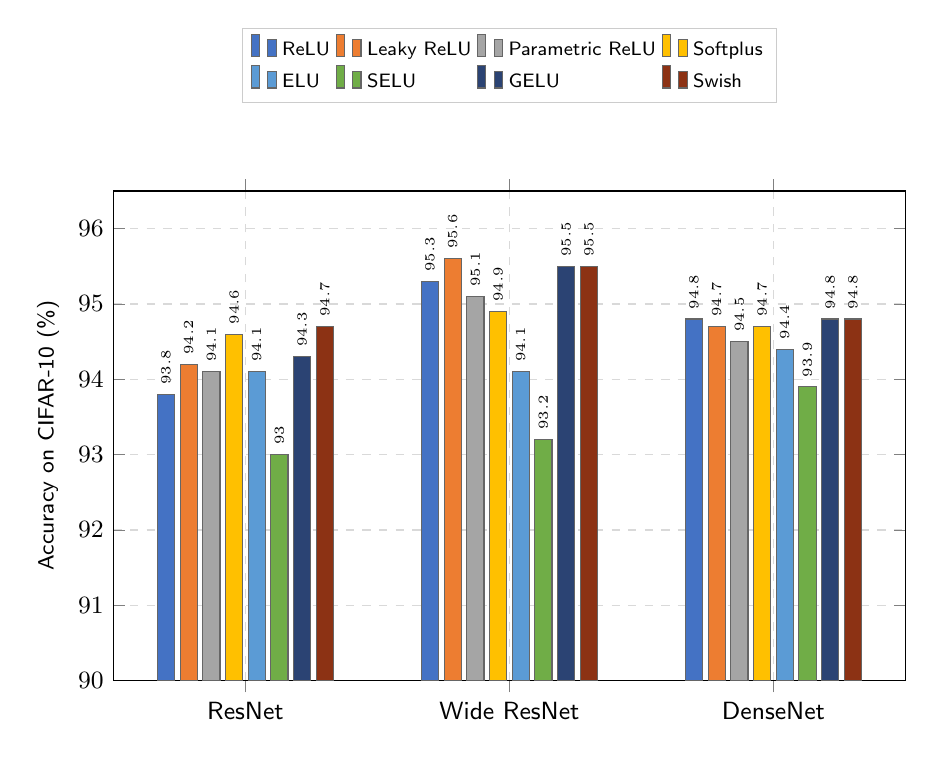
\begin{tikzpicture}
% Define exact color palette matching lecture slide
\definecolor{cReLU}{RGB}{68, 114, 196}
\definecolor{cLeaky}{RGB}{237, 125, 49}
\definecolor{cPReLU}{RGB}{165, 165, 165}
\definecolor{cSoftplus}{RGB}{255, 192, 0}
\definecolor{cELU}{RGB}{91, 155, 213}
\definecolor{cSELU}{RGB}{112, 173, 71}
\definecolor{cGELU}{RGB}{43, 67, 115}
\definecolor{cSwish}{RGB}{140, 50, 20}

\begin{axis}[
    ybar,
    bar width=6.2pt,
    width=0.96\textwidth,
    height=7.8cm,
    ymin=90, ymax=96.5,
    ylabel={Accuracy on CIFAR-10 (\%)},
    ylabel style={font=\footnotesize\sffamily},
    symbolic x coords={ResNet, Wide ResNet, DenseNet},
    xtick=data,
    tick label style={font=\small\sffamily},
    nodes near coords,
    nodes near coords style={font=\tiny\sffamily, rotate=90, anchor=west},
    enlarge x limits=0.25,
    legend style={at={(0.5,1.18)}, anchor=south, legend columns=4, font=\scriptsize\sffamily, fill=white, draw=gray!40},
    legend cell align={left},
    grid=major,
    grid style={dashed, gray!30},
    ymajorgrids=true,
]
% 1. ReLU
\addplot[fill=cReLU, draw=black!60] coordinates {(ResNet,93.8) (Wide ResNet,95.3) (DenseNet,94.8)};
% 2. Leaky ReLU
\addplot[fill=cLeaky, draw=black!60] coordinates {(ResNet,94.2) (Wide ResNet,95.6) (DenseNet,94.7)};
% 3. Parametric ReLU
\addplot[fill=cPReLU, draw=black!60] coordinates {(ResNet,94.1) (Wide ResNet,95.1) (DenseNet,94.5)};
% 4. Softplus
\addplot[fill=cSoftplus, draw=black!60] coordinates {(ResNet,94.6) (Wide ResNet,94.9) (DenseNet,94.7)};
% 5. ELU
\addplot[fill=cELU, draw=black!60] coordinates {(ResNet,94.1) (Wide ResNet,94.1) (DenseNet,94.4)};
% 6. SELU
\addplot[fill=cSELU, draw=black!60] coordinates {(ResNet,93.0) (Wide ResNet,93.2) (DenseNet,93.9)};
% 7. GELU
\addplot[fill=cGELU, draw=black!60] coordinates {(ResNet,94.3) (Wide ResNet,95.5) (DenseNet,94.8)};
% 8. Swish
\addplot[fill=cSwish, draw=black!60] coordinates {(ResNet,94.7) (Wide ResNet,95.5) (DenseNet,94.8)};

\legend{ReLU, Leaky ReLU, Parametric ReLU, Softplus, ELU, SELU, GELU, Swish}
\end{axis}
\end{tikzpicture}
\caption{Empirical accuracy comparison of 8 modern activation functions across ResNet, Wide ResNet, and DenseNet on CIFAR-10 (originating from Ramachandran et al.~\cite{ramachandran2017searching}). The benchmark highlights two foundational empirical realities: (1) Deprecated activations (Sigmoid and Tanh) are omitted entirely because they suffer from catastrophic gradient vanishing and fail to train; (2) The performance variance across all modern ReLU variants is remarkably narrow ($\le 1.0\%$), proving that activation selection is almost never the primary source of error in an underperforming deep model.}
\label{fig:cifar10_activation_benchmark}
\end{figure}

\subsection{Diagnostic principles for activations}
\label{sec:activation_empirical_benchmark}

Table~\ref{tab:activation_functions_master_comparison} provides a comprehensive master comparative taxonomy of all discussed activation functions, summarizing their mathematical formulations, output dynamic ranges, key computational properties, and practical engineering verdicts.

\begin{table}[H]
\centering
\small
\caption{Comparative theoretical taxonomy of neural activation functions.}
\label{tab:activation_functions_master_comparison}
\begin{tabularx}{\textwidth}{l l c p{3.8cm} X}
\toprule
\textbf{Activation} & \textbf{Formula $f(z)$} & \textbf{Range} & \textbf{Key Properties} & \textbf{Diagnostic Role \& Practical Recommendation} \\
\midrule
\textbf{Sigmoid} & $\frac{1}{1 + e^{-z}}$ & $(0, 1)$ & Non-zero centered, saturates & \textbf{Deprecated for hidden layers}. Severe vanishing gradients ($\sigma' \le 0.25$); binary output heads only. \\
\addlinespace
\textbf{Tanh} & $\frac{e^z - e^{-z}}{e^z + e^{-z}}$ & $(-1, 1)$ & Zero-centered, saturates & \textbf{Deprecated for deep nets}. Solves centering, but saturation kills deep gradients ($\tanh' \to 0$). \\
\addlinespace
\textbf{ReLU} & $\max(0, z)$ & $[0, \infty)$ & Non-saturating ($z>0$), dying risk & \textbf{Universal Industry Standard}. $6\times$ GPU speedup, constant unit gradient; default starting baseline. \\
\addlinespace
\textbf{Leaky ReLU} & $\max(\alpha z, z)$ & $(-\infty, \infty)$ & Non-saturating, slope $\alpha = 0.01$ & \textbf{Robust Alternative}. Completely eliminates dying ReLU trap with trivial compute overhead. \\
\addlinespace
\textbf{PReLU} & $\max(\alpha z, z)$ & $(-\infty, \infty)$ & Learnable negative slope $\alpha$ & \textbf{Adaptive Slope}. Backpropagates into $\alpha$ at $+1$ parameter per feature channel. \\
\addlinespace
\textbf{ELU} & $\begin{cases} z & z > 0 \\ \alpha(e^z - 1) & z \le 0 \end{cases}$ & $(-\alpha, \infty)$ & Smooth, mean near 0, saturates left & \textbf{Noise Robust}. Negative saturation provides noise immunity; requires exponential. \\
\addlinespace
\textbf{GELU} & $z \Phi(z)$ & $[-0.17, \infty)$ & Smooth, non-monotonic dip & \textbf{Transformer Standard}. Probabilistic gating; default in BERT, GPT, and Vision Transformers. \\
\addlinespace
\textbf{Swish} & $z \cdot \sigma(\beta z)$ & $[-0.28, \infty)$ & Smooth, non-monotonic dip & \textbf{NAS Discovery}. Matches or slightly exceeds ReLU on deep ResNets ($\beta = 1$). \\
\bottomrule
\end{tabularx}
\end{table}

In empirical deep learning engineering, diagnostic reasoning regarding activation functions involves contrasting two fundamentally distinct performance scenarios:

\paragraph{1. The Catastrophic Failure of Deprecated Activations (Sigmoid and Tanh):}
If an engineer selects Sigmoid or Tanh for the hidden layers of a modern deep architecture (such as a 50-layer ResNet), \textbf{the performance will drop catastrophically}. In most cases, the model will fail to learn entirely, halting at random guessing accuracy. As derived in Section~\ref{sec:sigmoid_tanh_pathologies}, because $|\sigma'(z)| \le 0.25$, gradients decay exponentially across cascading layers as $\sim (0.25)^{50} \approx 7.8 \times 10^{-31}$. Early layers receive strictly zero update, freezing the network at its random initialization. This is why Sigmoid and Tanh are omitted completely from competitive benchmarks such as Figure~\ref{fig:cifar10_activation_benchmark}: they cannot converge on deep feedforward topologies without specialized layer-wise pre-training.

\paragraph{2. The Narrow Margin of Rectifiers: Activation Choice is Not the Source of Error:}
In stark contrast, when comparing modern non-saturating rectifiers (ReLU, Leaky ReLU, PReLU, ELU, GELU, Swish), the empirical results in Figure~\ref{fig:cifar10_activation_benchmark} reveal that \textbf{all variants cluster within a remarkably narrow $\pm 0.5\%$--$1.0\%$ accuracy margin}:
\begin{itemize}[noitemsep,topsep=2pt,parsep=0pt,partopsep=0pt]
  \item On ResNet: ReLU ($93.8\%$) vs. Leaky ReLU ($94.2\%$) vs. Swish ($94.7\%$).
  \item On Wide ResNet: ReLU ($95.3\%$) vs. Leaky ReLU ($95.6\%$) vs. GELU ($95.5\%$).
  \item On DenseNet: ReLU ($94.8\%$) vs. Leaky ReLU ($94.7\%$) vs. GELU ($94.8\%$).
\end{itemize}

This empirical reality leads to a foundational diagnostic principle in machine learning:
\begin{quote}
\textbf{If a deep neural network is achieving poor performance, suffering from severe underfitting, or failing to converge when using standard ReLU, the activation function is almost certainly NOT the source of error.}
\end{quote}
Switching from standard ReLU to Leaky ReLU, ELU, or GELU will never rescue a broken model. The validity of this assessment is directly demonstrated by Figure~\ref{fig:cifar10_activation_benchmark}: the performance differences among all 8 modern activation functions across three distinct network families are minimal. A network suffering from flawed convergence cannot be repaired by altering the activation function.

When a deep architecture fails or underperforms, the engineer must look past the activation function and systematically diagnose the \textbf{true foundational pillars of deep training}:
\begin{enumerate}[leftmargin=*]
  \item \textbf{Learning Rate Misconfiguration}: Is the learning rate $\eta$ excessively high, causing numerical divergence or knocking neurons into the dying ReLU trap? Or is it excessively low, causing the optimizer to stall in flat regions?
  \item \textbf{Improper Weight Initialization}: Were weights initialized with unscaled Gaussian noise rather than He/Kaiming variance-preserving initialization (derived in Section~\ref{sec:weight_initialization_theory}), causing activation variances to vanish or explode during the very first forward pass?
  \item \textbf{Missing or Misplaced Normalization Layers}: Is the network lacking Batch Normalization or Layer Normalization (Section~\ref{sec:batch_normalization_theory}), allowing internal covariate shift and gradient scale imbalances to destabilize deeper representations?
  \item \textbf{Input Data Misconditioning}: Were input images fed as unnormalized $[0, 255]$ integer values rather than being zero-centered and scaled by channel-wise standard deviations (Section~\ref{sec:data_preprocessing_conditioning})?
  \item \textbf{Optimization Scheduling and Regularization}: Is the optimizer lacking learning rate warmup, momentum, or cosine annealing (Section~\ref{sec:training_dynamics_babysitting}), or is the generalization gap driven by insufficient data augmentation or mismatched weight decay?
\end{enumerate}

\paragraph{The Practical Baseline Rule:}
In industrial and research practice, the golden rule is: \textbf{Default to standard ReLU}. ReLU is computationally trivial (a single hardware branch comparator), memory-efficient, and universally accelerated across edge devices, GPUs, and TPUs. Only when the entire deep learning system is verified to be fully functional, converging stably, and properly regularized should an engineer experiment with Leaky ReLU, ELU, GELU, or Swish to harvest the final marginal fractions of a percent on benchmark competitions.

\section{Input preprocessing and conditioning}
\label{sec:data_preprocessing_conditioning}

Before any architectural forward pass or backpropagation update can occur, the input data feeding the network must undergo rigorous mathematical conditioning. In real-world applications, raw data rarely arrives in a form amenable to smooth gradient-based optimization. In computer vision, raw digital images arrive as unsigned 8-bit integers in the discrete range $\{0, 1, \dots, 255\}$; in tabular, speech, and multimodal datasets, features frequently span wildly disparate dynamic ranges, arbitrary non-zero offsets, and dense cross-feature correlations.

Training a deep neural network directly on raw, unconditioned input data triggers severe pathologies across the entire optimization trajectory:
\begin{enumerate}[leftmargin=*]
  \item \textbf{Directional Gradient Locking and Zigzagging}: When raw features are strictly positive (such as pixel intensities $x_i \in [0, 255]$), all incoming weights connected to a first-layer neuron receive gradient updates of identical sign. The optimizer is prevented from navigating into mixed-sign parameter quadrants, forcing it into slow, high-frequency oscillations across the loss surface.
  \item \textbf{Extreme Loss Surface Eccentricity}: Disparities in raw feature magnitudes distort the local curvature of the objective function. The Hessian matrix develops an extreme condition number $\kappa(\mathbf{H}) = \lambda_{\max} / \lambda_{\min} \gg 1$, creating steep, narrow ravines where first-order gradient descent oscillates violently across the walls while making negligible progress along the base.
  \item \textbf{Premature Activation Saturation}: Feeding unscaled, large raw inputs into the initial layers pushes pre-activations to extreme values ($|z| \gg 1$), shoving classical saturating activations into their zero-derivative asymptotes and destabilizing rectifier activations with large forward scale shifts.
  \item \textbf{Arbitrary Sensitivity to Measurement Units}: Unnormalized models lack scale invariance; scaling a single feature from meters to millimeters multiplies its gradient magnitude by $10^3$, completely overturning the learning rate calibration across dimensions.
\end{enumerate}

To overcome these obstacles, machine learning practitioners employ a systematic taxonomy of preprocessing operations on raw data matrices $\mathbf{X} \in \mathbb{R}^{N \times D}$:
\begin{itemize}[noitemsep,topsep=2pt,parsep=0pt,partopsep=0pt]
  \item \textbf{Zero-Centering (Mean Subtraction)}: Translates the empirical centroid of the dataset to the coordinate origin ($\mathbb{E}[\mathbf{x}] = \mathbf{0}$), eliminating sign coupling.
  \item \textbf{Variance Rescaling (Standardization / Z-Score)}: Scales each coordinate dimension to unit empirical variance ($\operatorname{Var}(x_d) = 1$), equalizing diagonal curvature.
  \item \textbf{Min-Max Normalization (Feature Rescaling)}: Linearly maps bounded features into a normalized compact interval, such as $[0, 1]$ or $[-1, 1]$.
  \item \textbf{Principal Component Analysis (PCA Decorrelation)}: Rotates the data onto the orthogonal eigenvector basis of its covariance matrix, annihilating all off-diagonal linear cross-correlations.
  \item \textbf{Whitening (Sphering Transformation)}: Scales decorrelated principal components by the inverse square root of their eigenvalues, yielding an isotropic identity covariance matrix ($\operatorname{Cov}(\mathbf{x}_{\text{white}}) = \mathbf{I}$).
  \item \textbf{Local Contrast / Patch Normalization}: Normalizes spatial neighborhoods by local standard deviations, suppressing illumination variations in vision.
\end{itemize}

\subsection{Centering and variance scaling}
\label{sec:zero_centering_scaling}

The two primary operations in feature conditioning are zero-centering and variance scaling. To understand their necessity, we examine their optimization consequences from both qualitative and quantitative perspectives.

\paragraph{1. Motivation of Zero-Centering: Eliminating Sign Coupling and Hessian Spread.}
\begin{itemize}[leftmargin=*]
  \item \textbf{Qualitative Perspective}: If input features are uncentered and strictly positive (as is universal for raw image pixels $x \in [0, 255]$), every weight connected to an initial neuron is forced to change in the same direction. The optimizer cannot increase one weight while decreasing another in a single update step. If the loss minimum requires opposing sign adjustments, gradient descent is forced into an inefficient zigzagging pattern, bouncing back and forth across parameter quadrants.
  \item \textbf{Quantitative Derivation (Gradient Sign Coupling)}: Consider a neuron computing pre-activation $a = \mathbf{w}^\top \mathbf{x} + b$. By the multivariate chain rule, the gradient of the scalar loss $\mathcal{L}$ with respect to the weight vector $\mathbf{w} \in \mathbb{R}^D$ is:
    \begin{equation}
    \nabla_{\mathbf{w}} \mathcal{L} = \frac{\partial \mathcal{L}}{\partial a} \frac{\partial a}{\partial \mathbf{w}} = \delta \mathbf{x},
    \label{eq:grad_weight_vector_chain}
    \end{equation}
    where $\delta \equiv \frac{\partial \mathcal{L}}{\partial a} \in \mathbb{R}$ is the scalar error adjoint. The sign of each individual partial derivative is:
    \begin{equation}
    \operatorname{sign}\left( \frac{\partial \mathcal{L}}{\partial w_i} \right) = \operatorname{sign}(\delta) \cdot \operatorname{sign}(x_i).
    \end{equation}
    When $x_i > 0$ for all $i \in \{1, \dots, D\}$, every component of $\nabla_{\mathbf{w}} \mathcal{L}$ shares the exact sign of $\delta$:
    \begin{equation}
    \operatorname{sign}\left( \frac{\partial \mathcal{L}}{\partial w_i} \right) = \operatorname{sign}(\delta) \quad \forall i \in \{1, \dots, D\}.
    \label{eq:all_positive_grad_sign}
    \end{equation}
    The gradient vector $\nabla_{\mathbf{w}} \mathcal{L}$ is strictly confined to the positive cone $\mathcal{C}_+ = \{\mathbf{v} : v_i \ge 0\}$ or the negative cone $\mathcal{C}_- = \{\mathbf{v} : v_i \le 0\}$. As illustrated in Figure~\ref{fig:zigzag_gradient_descent}, if the optimum $\mathbf{w}^*$ requires coordinate updates of opposite signs ($w_1 \uparrow, w_2 \downarrow$), gradient descent cannot point toward $\mathbf{w}^*$ and is forced to oscillate diagonally.
  \item \textbf{Quantitative Derivation (Hessian Condition Number Expansion)}: In a local quadratic approximation of the loss $\mathcal{L}(\mathbf{w}) \approx \frac{1}{2N} \|\mathbf{X} \mathbf{w} - \mathbf{y}\|_2^2$, the Hessian matrix of second derivatives is:
    \begin{equation}
    \mathbf{H} = \frac{1}{N} \mathbf{X}^\top \mathbf{X} = \frac{1}{N} \sum_{n=1}^N \mathbf{x}_n \mathbf{x}_n^\top.
    \end{equation}
    If the dataset has an empirical non-zero mean vector $\boldsymbol{\mu} = \frac{1}{N}\sum_{n=1}^N \mathbf{x}_n \ne \mathbf{0}$, the second-moment matrix expands around the centered sample covariance $\boldsymbol{\Sigma} = \frac{1}{N} \sum_n (\mathbf{x}_n - \boldsymbol{\mu})(\mathbf{x}_n - \boldsymbol{\mu})^\top$:
    \begin{equation}
    \mathbf{H} = \boldsymbol{\Sigma} + \boldsymbol{\mu} \boldsymbol{\mu}^\top.
    \label{eq:hessian_mean_rank_one}
    \end{equation}
    The rank-one outer product $\boldsymbol{\mu} \boldsymbol{\mu}^\top$ adds an eigenvalue of magnitude $\|\boldsymbol{\mu}\|_2^2$ along the direction of $\boldsymbol{\mu}$. When raw features have large non-zero offsets (for example, raw pixels where $\mu_i \approx 128 \implies \|\boldsymbol{\mu}\|_2^2 \approx D \times 128^2$), the maximum eigenvalue of the Hessian inflates dramatically:
    \begin{equation}
    \lambda_{\max}(\mathbf{H}) \approx \lambda_{\max}(\boldsymbol{\Sigma}) + \|\boldsymbol{\mu}\|_2^2, \qquad \lambda_{\min}(\mathbf{H}) \approx \lambda_{\min}(\boldsymbol{\Sigma}).
    \end{equation}
    The resulting condition number of the Hessian explodes:
    \begin{equation}
    \kappa(\mathbf{H}) = \frac{\lambda_{\max}(\mathbf{H})}{\lambda_{\min}(\mathbf{H})} \approx \frac{\lambda_{\max}(\boldsymbol{\Sigma}) + \|\boldsymbol{\mu}\|_2^2}{\lambda_{\min}(\boldsymbol{\Sigma})} \gg 1.
    \label{eq:condition_number_uncentered}
    \end{equation}
    Since the convergence rate of first-order gradient descent is bounded by $\left( \frac{\kappa - 1}{\kappa + 1} \right)^2$, an uncentered non-zero mean $\boldsymbol{\mu}$ directly causes catastrophic optimization slowdown. Zero-centering sets $\boldsymbol{\mu} = \mathbf{0}$, annihilating the $\boldsymbol{\mu}\boldsymbol{\mu}^\top$ term and restoring $\mathbf{H} = \boldsymbol{\Sigma}$.
\end{itemize}

\begin{figure}[H]
\centering
\begin{tikzpicture}[scale=0.92]
  % Grid and axes
  \draw[->, thick, gray!70] (-3.8, 0) -- (3.8, 0) node[right, font=\sffamily\small] {$w_1$};
  \draw[->, thick, gray!70] (0, -3.2) -- (0, 3.5) node[above, font=\sffamily\small] {$w_2$};

  % Allowed gradient regions (shaded cones)
  \fill[examred!10] (0,0) -- (3.5, 3.5) -- (0, 3.5) -- cycle;
  \fill[examred!10] (0,0) -- (3.5, 3.5) -- (3.5, 0) -- cycle;
  \fill[examred!10] (0,0) -- (-3.5, -3.1) -- (0, -3.1) -- cycle;
  \fill[examred!10] (0,0) -- (-3.5, -3.1) -- (-3.5, 0) -- cycle;

  \node[font=\bfseries\sffamily\footnotesize, text=examred!80!black, align=center] at (2.2, 1.2) {Allowed Update\\Quadrant $(++)$};
  \node[font=\bfseries\sffamily\footnotesize, text=examred!80!black, align=center] at (-2.0, -1.5) {Allowed Update\\Quadrant $(--)$};

  % Prohibited zones
  \node[font=\sffamily\scriptsize, text=gray!80, align=center] at (-2.0, 2.0) {Prohibited Zone\\($\Delta w_1 < 0, \Delta w_2 > 0$)};
  \node[font=\sffamily\scriptsize, text=gray!80, align=center] at (2.0, -2.0) {Prohibited Zone\\($\Delta w_1 > 0, \Delta w_2 < 0$)};

  % Loss Contours (ellipses)
  \draw[politoNavy!40, thick, rotate around={-25:(1.5, 1.0)}] (1.5, 1.0) ellipse (0.7cm and 0.4cm);
  \draw[politoNavy!50, thick, rotate around={-25:(1.5, 1.0)}] (1.5, 1.0) ellipse (1.5cm and 0.8cm);
  \draw[politoNavy!60, thick, rotate around={-25:(1.5, 1.0)}] (1.5, 1.0) ellipse (2.3cm and 1.2cm);
  \draw[politoNavy!70, thick, rotate around={-25:(1.5, 1.0)}] (1.5, 1.0) ellipse (3.1cm and 1.6cm);

  % Optimum
  \node[circle, fill=politoNavy, inner sep=2pt] (opt) at (1.5, 1.0) {};
  \node[right=2pt of opt, font=\bfseries\sffamily\small, text=politoNavy] {$\mathbf{w}^*$ (Optimal)};

  % Start point
  \node[circle, fill=examred, inner sep=2.2pt] (p0) at (-2.6, 2.2) {};
  \node[above left=1pt of p0, font=\bfseries\sffamily\small, text=examred] {$\mathbf{w}^{(0)}$};

  % Hypothetical optimal direct direction
  \draw[-{Stealth[scale=1.2]}, dashed, thick, intuitiongreen!80!black] (p0) -- (opt) 
    node[midway, above, sloped, font=\bfseries\sffamily\scriptsize, text=intuitiongreen!80!black] {Direct unconstrained path};

  % Zigzag steps
  \coordinate (z1) at (-1.4, 2.9);
  \coordinate (z2) at (-1.9, 1.6);
  \coordinate (z3) at (-0.7, 2.3);
  \coordinate (z4) at (-1.1, 1.1);
  \coordinate (z5) at (0.2, 1.8);
  \coordinate (z6) at (-0.2, 0.7);
  \coordinate (z7) at (0.9, 1.4);
  \coordinate (z8) at (0.6, 0.7);
  \coordinate (z9) at (1.3, 1.1);

  \draw[-{Stealth}, very thick, examred] (p0) -- (z1);
  \draw[-{Stealth}, very thick, examred] (z1) -- (z2);
  \draw[-{Stealth}, very thick, examred] (z2) -- (z3);
  \draw[-{Stealth}, very thick, examred] (z3) -- (z4);
  \draw[-{Stealth}, very thick, examred] (z4) -- (z5);
  \draw[-{Stealth}, very thick, examred] (z5) -- (z6);
  \draw[-{Stealth}, very thick, examred] (z6) -- (z7);
  \draw[-{Stealth}, very thick, examred] (z7) -- (z8);
  \draw[-{Stealth}, very thick, examred] (z8) -- (z9);

  \node[font=\bfseries\sffamily\footnotesize, text=examred, align=left] at (-2.5, -2.5) {Forced zigzag path\\due to strictly positive $x_i > 0$};
\end{tikzpicture}
\caption{The geometric pathology of uncentered data. When input features are strictly positive ($x_i > 0$), parameter updates $\Delta \mathbf{w} = -\eta \frac{\partial \mathcal{L}}{\partial a} \mathbf{x}$ are restricted strictly to quadrants $(++)$ and $(--)$ (shaded regions). Reaching an optimum $\mathbf{w}^*$ situated in a mixed quadrant forces gradient descent into an inefficient, high-frequency zigzag trajectory. Zero-centering ($\mathbf{x} \leftarrow \mathbf{x} - \boldsymbol{\mu}$) eliminates this quadrant constraint, permitting direct gradient descent along the green dashed trajectory.}
\label{fig:zigzag_gradient_descent}
\end{figure}

\paragraph{2. Motivation of Variance Rescaling: Equalizing Axis Curvature.}
\begin{itemize}[leftmargin=*]
  \item \textbf{Qualitative Perspective}: If one input feature varies over thousands of units while another varies over fractional decimals, the loss surface forms an extremely steep, narrow canyon. Gradient updates with a uniform learning rate $\eta$ bounce uncontrollably between the steep walls (along the high-variance feature) while crawling with imperceptible slowness along the flat canyon floor (along the low-variance feature).
  \item \textbf{Quantitative Derivation (Curvature Equalization)}: The diagonal elements of the Hessian matrix correspond directly to the second moments of the individual feature dimensions:
    \begin{equation}
    H_{ii} = \frac{\partial^2 \mathcal{L}}{\partial w_i^2} = \frac{1}{N} \sum_{n=1}^N x_{ni}^2 \approx \sigma_i^2 \quad (\text{for zero-centered features}).
    \end{equation}
    If feature 1 has variance $\sigma_1^2$ and feature 2 has variance $\sigma_2^2$ with $\sigma_1 \gg \sigma_2$, the condition number satisfies $\kappa(\mathbf{H}) \ge \sigma_1^2 / \sigma_2^2$. The maximum stable learning rate is upper-bounded by the steepest curvature:
    \begin{equation}
    \eta < \frac{2}{\lambda_{\max}(\mathbf{H})} \approx \frac{2}{\sigma_1^2}.
    \end{equation}
    Under this small learning rate $\eta$, the parameter progress along the flat dimension $w_2$ per iteration is:
    \begin{equation}
    \Delta w_2 \approx -\eta \sigma_2^2 w_2 < -\frac{2 \sigma_2^2}{\sigma_1^2} w_2,
    \end{equation}
    requiring $\mathcal{O}\left( \frac{\sigma_1^2}{\sigma_2^2} \right)$ update steps to converge. Dividing each feature by its empirical standard deviation $\sigma_i$ scales the diagonal entries of the Hessian to $H_{ii} \approx 1$, equalizing axis curvature and enabling rapid, balanced convergence.
\end{itemize}

\paragraph{3. Evolution of Visual Normalization Conventions.}
In deep convolutional architectures, input preprocessing standards have evolved across model generations, transitioning from full 3D spatial images toward compact channel-wise scaling:
\begin{table}[H]
\centering
\small
\begin{tabular}{@{}llll@{}}
\toprule
\textbf{Architecture} & \textbf{Normalization Protocol} & \textbf{Statistics Shape} & \textbf{Practical Implementation} \\ \midrule
\textbf{AlexNet (2012)} & Full Mean Image Subtraction & $[H \times W \times C]$ & $\mathbf{x} \leftarrow \mathbf{x} - \bar{\mathbf{X}}_{\text{pixel}}$ \\
\textbf{VGGNet (2014)} & Per-Channel Mean Subtraction & $[3]$ (RGB scalars) & $\mathbf{x}_c \leftarrow \mathbf{x}_c - \mu_c$ \\
\textbf{ResNet (2015)} & Per-Channel Mean and Std Scaling & $[3]$ means, $[3]$ stds & $\mathbf{x}_c \leftarrow (\mathbf{x}_c - \mu_c) / \sigma_c$ \\ \bottomrule
\end{tabular}
\caption{Comparison of input image preprocessing standards across landmark deep visual architectures. While early networks subtracted full 3D mean images, modern standard practice subtracts per-channel RGB means and scales by per-channel standard deviations.}
\label{tab:cnn_preprocessing_standards}
\end{table}

\begin{examinsight}[Rule of Thumb for Image Preprocessing]
For visual image recognition, the empirical golden rule is: \textbf{center only, or standardize per-channel}. Never attempt full dataset variance normalization across arbitrary dimensions, and never apply PCA whitening.
\end{examinsight}

\paragraph{Mathematical Definition of Centering and Variance Scaling:}
Formally, let $\mathbf{x} \in \mathbb{R}^D$ denote an input feature vector. The standard preprocessing pipeline applies two consecutive linear transformations:
\begin{equation}
\mathbf{x}_{\text{centered}} = \mathbf{x} - \boldsymbol{\mu}, \qquad \mathbf{x}_{\text{norm}} = \frac{\mathbf{x} - \boldsymbol{\mu}}{\boldsymbol{\sigma}},
\label{eq:centering_and_scaling}
\end{equation}
where $\boldsymbol{\mu} = \frac{1}{N}\sum_{i=1}^N \mathbf{x}_i$ is the empirical dataset mean vector, and $\boldsymbol{\sigma} = \sqrt{\frac{1}{N}\sum_{i=1}^N (\mathbf{x}_i - \boldsymbol{\mu})^2}$ is the empirical standard deviation vector (computed element-wise).

Figure~\ref{fig:centering_scaling_geometry} visually demonstrates the geometric progression of these two transformations on a two-dimensional feature distribution.

\begin{figure}[H]
\centering
\begin{tikzpicture}[scale=0.82]
  % Stage 1: Raw Data
  \begin{scope}[shift={(0,0)}]
    \draw[->, thick, gray!70] (-0.5,0) -- (4.2,0) node[right, font=\tiny\sffamily] {$x_1$};
    \draw[->, thick, gray!70] (0,-0.5) -- (0,3.8) node[above, font=\tiny\sffamily] {$x_2$};
    \fill[examred!15, rotate around={35:(2.2,2.0)}] (2.2,2.0) ellipse (1.6cm and 0.6cm);
    \draw[examred, thick, rotate around={35:(2.2,2.0)}] (2.2,2.0) ellipse (1.6cm and 0.6cm);
    \fill[examred] (2.2,2.0) circle (2pt) node[above right, font=\tiny\bfseries] {$\boldsymbol{\mu} \ne \mathbf{0}$};
    \draw[dashed, gray] (2.2,0) -- (2.2,2.0) -- (0,2.0);
    \node[below, font=\tiny] at (2.2,0) {$\mu_1$};
    \node[left, font=\tiny] at (0,2.0) {$\mu_2$};
    \node[font=\footnotesize\bfseries\sffamily, text=politoNavy] at (1.8,-1.0) {(a) Raw Data};
    \node[font=\tiny\sffamily, text=gray!80, align=center] at (1.8,-1.5) {$\boldsymbol{\mu} \ne \mathbf{0}, \sigma_1 \ne \sigma_2$\\Quadrant restricted};
  \end{scope}

  % Arrow 1
  \draw[-{Stealth[length=2mm]}, very thick, politoNavy] (4.4,1.8) -- (5.6,1.8) 
    node[midway, above, font=\tiny\bfseries\sffamily] {$-\boldsymbol{\mu}$};

  % Stage 2: Centered Data
  \begin{scope}[shift={(7.5,1.8)}]
    \draw[->, thick, gray!70] (-2.2,0) -- (2.4,0) node[right, font=\tiny\sffamily] {$x_1$};
    \draw[->, thick, gray!70] (0,-2.0) -- (0,2.2) node[above, font=\tiny\sffamily] {$x_2$};
    \fill[orange!15, rotate around={35:(0,0)}] (0,0) ellipse (1.6cm and 0.6cm);
    \draw[orange!90!black, thick, rotate around={35:(0,0)}] (0,0) ellipse (1.6cm and 0.6cm);
    \fill[orange!90!black] (0,0) circle (2pt) node[below right, font=\tiny\bfseries] {$\boldsymbol{\mu} = \mathbf{0}$};
    \node[font=\footnotesize\bfseries\sffamily, text=politoNavy] at (0,-2.8) {(b) Zero-Centered};
    \node[font=\tiny\sffamily, text=gray!80, align=center] at (0,-3.3) {$\mathbb{E}[\mathbf{x}] = \mathbf{0}$, free signs\\$\sigma_1 \ne \sigma_2$ (eccentric)};
  \end{scope}

  % Arrow 2
  \draw[-{Stealth[length=2mm]}, very thick, politoNavy] (9.9,1.8) -- (11.1,1.8) 
    node[midway, above, font=\tiny\bfseries\sffamily] {$/\boldsymbol{\sigma}$};

  % Stage 3: Standardized Data
  \begin{scope}[shift={(13.0,1.8)}]
    \draw[->, thick, gray!70] (-2.0,0) -- (2.2,0) node[right, font=\tiny\sffamily] {$\hat{x}_1$};
    \draw[->, thick, gray!70] (0,-2.0) -- (0,2.2) node[above, font=\tiny\sffamily] {$\hat{x}_2$};
    \fill[intuitiongreen!15] (0,0) circle (1.1cm);
    \draw[intuitiongreen, thick] (0,0) circle (1.1cm);
    \fill[intuitiongreen] (0,0) circle (2pt) node[below right, font=\tiny\bfseries] {$\boldsymbol{\mu} = \mathbf{0}$};
    \draw[<->, dashed, intuitiongreen!80!black] (0,0) -- (1.1,0) node[midway, above, font=\tiny] {$\sigma_1=1$};
    \draw[<->, dashed, intuitiongreen!80!black] (0,0) -- (0,1.1) node[midway, right, font=\tiny] {$\sigma_2=1$};
    \node[font=\footnotesize\bfseries\sffamily, text=politoNavy] at (0,-2.8) {(c) Standardized};
    \node[font=\tiny\sffamily, text=gray!80, align=center] at (0,-3.3) {$\sigma_1 = \sigma_2 = 1$\\Equalized diagonal $H_{ii}$};
  \end{scope}
\end{tikzpicture}
\caption{The geometric progression of feature conditioning. (a) Raw input features are situated in the positive quadrant with non-zero mean $\boldsymbol{\mu} \ne \mathbf{0}$ and unequal variances $\sigma_1 \ne \sigma_2$. (b) Zero-centering subtracts $\boldsymbol{\mu}$, shifting the empirical centroid to the origin $(0, 0)$ and restoring full 360-degree gradient directional freedom. (c) Variance scaling divides by $\boldsymbol{\sigma}$, normalizing variances to 1 along all coordinate axes and equalizing the diagonal curvature of the loss surface.}
\label{fig:centering_scaling_geometry}
\end{figure}

\subsection{PCA and whitening}
\label{sec:pca_and_whitening}

While zero-centering and coordinate-wise variance scaling normalize each dimension independently, they operate strictly along the canonical coordinate axes. In real-world data, features frequently exhibit strong cross-correlations. To tackle this, we examine PCA and Whitening from qualitative and quantitative perspectives.

\paragraph{1. Motivation of PCA and Whitening: Oblique Correlations and Complete Sphering.}
\begin{itemize}[leftmargin=*]
  \item \textbf{Qualitative Perspective}: Standard variance standardization scales the bounding box of the data along the $x_1$ and $x_2$ axes. However, if $x_1$ and $x_2$ are strongly correlated (such as adjacent pixels in an image or correlated physical measurements), the data cloud forms an oblique, tilted ellipse. In this case, the Hessian matrix contains large off-diagonal entries, causing gradient descent to oscillate across the tilted ridge. PCA decorrelation rotates the coordinate frame to align with the ellipse's principal axes, and Whitening stretches every axis to unit variance, turning the elliptical ravine into a perfectly round spherical bowl where gradient descent points straight to the minimum.
  \item \textbf{Quantitative Derivation (Eigendecomposition and Decorrelation)}: Given a zero-centered data matrix $\mathbf{X} \in \mathbb{R}^{N \times D}$, the empirical sample covariance matrix is:
    \begin{equation}
    \boldsymbol{\Sigma} = \frac{1}{N} \mathbf{X}^\top \mathbf{X} \in \mathbb{R}^{D \times D}.
    \label{eq:covariance_matrix}
    \end{equation}
    Because $\boldsymbol{\Sigma}$ is real, symmetric, and positive semi-definite, the spectral theorem guarantees an orthonormal eigendecomposition:
    \begin{equation}
    \boldsymbol{\Sigma} = \mathbf{U} \boldsymbol{\Lambda} \mathbf{U}^\top,
    \end{equation}
    where $\mathbf{U} \in \mathbb{R}^{D \times D}$ is an orthogonal matrix whose columns $\mathbf{u}_1, \dots, \mathbf{u}_D$ are the orthonormal eigenvectors ($\mathbf{U}^\top \mathbf{U} = \mathbf{I}$), and $\boldsymbol{\Lambda} = \operatorname{diag}(\lambda_1, \dots, \lambda_D)$ contains the non-negative eigenvalues representing the variance along each principal axis ($\lambda_1 \ge \lambda_2 \ge \dots \ge \lambda_D \ge 0$).
  \item \textbf{Quantitative Derivation (Whitening and Isotropic Hessian)}:
    Projecting the zero-centered data onto the eigenvector basis defines the PCA-rotated representation:
    \begin{equation}
    \mathbf{x}_{\text{rot}} = \mathbf{U}^\top \mathbf{x}.
    \label{eq:pca_projection}
    \end{equation}
    The covariance of $\mathbf{x}_{\text{rot}}$ is completely diagonalized:
    \begin{equation}
    \operatorname{Cov}(\mathbf{x}_{\text{rot}}) = \frac{1}{N} \mathbf{U}^\top \mathbf{X}^\top \mathbf{X} \mathbf{U} = \mathbf{U}^\top (\mathbf{U} \boldsymbol{\Lambda} \mathbf{U}^\top) \mathbf{U} = \boldsymbol{\Lambda}.
    \end{equation}
    All off-diagonal linear correlations are completely eliminated: $\operatorname{Cov}(x_{\text{rot}, i}, x_{\text{rot}, j}) = 0$ for all $i \ne j$.
    
    The whitening transformation subsequently scales each decorrelated principal coordinate by the inverse square root of its eigenvalue:
    \begin{equation}
    \mathbf{x}_{\text{white}} = \boldsymbol{\Lambda}^{-1/2} \mathbf{x}_{\text{rot}} = \boldsymbol{\Lambda}^{-1/2} \mathbf{U}^\top \mathbf{x}.
    \label{eq:whitening_transformation}
    \end{equation}
    The covariance matrix of the whitened representation evaluates to the exact identity matrix:
    \begin{equation}
    \operatorname{Cov}(\mathbf{x}_{\text{white}}) = \boldsymbol{\Lambda}^{-1/2} \operatorname{Cov}(\mathbf{x}_{\text{rot}}) \boldsymbol{\Lambda}^{-1/2} = \boldsymbol{\Lambda}^{-1/2} \boldsymbol{\Lambda} \boldsymbol{\Lambda}^{-1/2} = \mathbf{I}_D.
    \label{eq:whitened_identity_cov}
    \end{equation}
    Consequently, the empirical Hessian matrix of a quadratic objective computed on whitened features is perfectly isotropic:
    \begin{equation}
    \mathbf{H}_{\text{white}} = \frac{1}{N} \mathbf{X}_{\text{white}}^\top \mathbf{X}_{\text{white}} = \mathbf{I}_D \implies \kappa(\mathbf{H}_{\text{white}}) = \frac{\lambda_{\max}}{\lambda_{\min}} = 1.
    \end{equation}
    With a condition number of exactly $1$, the loss surface consists of concentric hyperspherical contours. The negative gradient vector points directly toward the global minimum $\mathbf{w}^*$, enabling gradient descent with learning rate $\eta = 1$ to converge in a single step!
\end{itemize}

Figure~\ref{fig:pca_whitening_geometry} illustrates the mathematical progression from correlated zero-centered data to decorrelated PCA coordinates and finally to the isotropic whitened distribution.

\begin{figure}[H]
\centering
\begin{tikzpicture}[scale=0.82]
  % Stage 1: Correlated zero-centered
  \begin{scope}[shift={(0,0)}]
    \draw[->, thick, gray!70] (-2.2,0) -- (2.4,0) node[right, font=\tiny\sffamily] {$x_1$};
    \draw[->, thick, gray!70] (0,-2.0) -- (0,2.2) node[above, font=\tiny\sffamily] {$x_2$};
    \fill[deepblue!15, rotate around={38:(0,0)}] (0,0) ellipse (1.8cm and 0.55cm);
    \draw[deepblue, thick, rotate around={38:(0,0)}] (0,0) ellipse (1.8cm and 0.55cm);
    \draw[-{Stealth[length=2mm]}, very thick, examred] (0,0) -- (1.42, 1.11) 
      node[above left, font=\tiny\bfseries] {$\mathbf{u}_1 \, (\lambda_1)$};
    \draw[-{Stealth[length=2mm]}, very thick, intuitiongreen] (0,0) -- (-0.34, 0.43) 
      node[above left, font=\tiny\bfseries] {$\mathbf{u}_2 \, (\lambda_2)$};
    \node[font=\footnotesize\bfseries\sffamily, text=politoNavy] at (0,-2.6) {(a) Correlated};
    \node[font=\tiny\sffamily, text=gray!80, align=center] at (0,-3.1) {$\Sigma_{12} \ne 0$, oblique\\Hessian off-diagonals};
  \end{scope}

  % Arrow 1
  \draw[-{Stealth[length=2mm]}, very thick, politoNavy] (2.7,0) -- (3.9,0) 
    node[midway, above, font=\tiny\bfseries\sffamily] {$\mathbf{U}^\top \mathbf{x}$};

  % Stage 2: PCA Rotated / Decorrelated
  \begin{scope}[shift={(6.2,0)}]
    \draw[->, thick, gray!70] (-2.2,0) -- (2.4,0) node[right, font=\tiny\sffamily] {$z_1$};
    \draw[->, thick, gray!70] (0,-2.0) -- (0,2.2) node[above, font=\tiny\sffamily] {$z_2$};
    \fill[orange!15] (0,0) ellipse (1.8cm and 0.55cm);
    \draw[orange!90!black, thick] (0,0) ellipse (1.8cm and 0.55cm);
    \draw[<->, dashed, orange!90!black] (-1.8,0) -- (1.8,0) node[pos=0.85, above, font=\tiny] {$\sqrt{\lambda_1}$};
    \draw[<->, dashed, orange!90!black] (0,-0.55) -- (0,0.55) node[pos=0.85, right, font=\tiny] {$\sqrt{\lambda_2}$};
    \node[font=\footnotesize\bfseries\sffamily, text=politoNavy] at (0,-2.6) {(b) PCA Decorrelated};
    \node[font=\tiny\sffamily, text=gray!80, align=center] at (0,-3.1) {$\operatorname{Cov}(\mathbf{z}) = \boldsymbol{\Lambda}$ (diagonal)\\Rotated to eigenbasis};
  \end{scope}

  % Arrow 2
  \draw[-{Stealth[length=2mm]}, very thick, politoNavy] (8.9,0) -- (10.1,0) 
    node[midway, above, font=\tiny\bfseries\sffamily] {$\boldsymbol{\Lambda}^{-1/2}$};

  % Stage 3: Whitened
  \begin{scope}[shift={(12.2,0)}]
    \draw[->, thick, gray!70] (-2.0,0) -- (2.2,0) node[right, font=\tiny\sffamily] {$x_{\text{w},1}$};
    \draw[->, thick, gray!70] (0,-2.0) -- (0,2.2) node[above, font=\tiny\sffamily] {$x_{\text{w},2}$};
    \fill[intuitiongreen!15] (0,0) circle (1.1cm);
    \draw[intuitiongreen, thick] (0,0) circle (1.1cm);
    \fill[intuitiongreen] (0,0) circle (2pt);
    \draw[<->, dashed, intuitiongreen!80!black] (0,0) -- (1.1,0) node[midway, above, font=\tiny] {$r=1$};
    \node[font=\footnotesize\bfseries\sffamily, text=politoNavy] at (0,-2.6) {(c) Whitened (Sphered)};
    \node[font=\tiny\sffamily, text=gray!80, align=center] at (0,-3.1) {$\operatorname{Cov}(\mathbf{x}_{\text{w}}) = \mathbf{I}$, $\kappa = 1$\\Spherical loss contours};
  \end{scope}
\end{tikzpicture}
\caption{The geometric mechanism of PCA decorrelation and whitening. (a) Correlated zero-centered data forming an oblique ellipse with eigenvectors $\mathbf{u}_1, \mathbf{u}_2$ and eigenvalues $\lambda_1, \lambda_2$. (b) PCA projection ($\mathbf{U}^\top \mathbf{x}$) rotates the coordinate system into the principal eigenbasis, eliminating cross-covariance ($\operatorname{Cov}(\mathbf{z}) = \boldsymbol{\Lambda}$). (c) Whitening ($\boldsymbol{\Lambda}^{-1/2} \mathbf{U}^\top \mathbf{x}$) scales each principal component by $1/\sqrt{\lambda_i}$, yielding an isotropic unit hypersphere where the Hessian condition number is $\kappa = 1$.}
\label{fig:pca_whitening_geometry}
\end{figure}

\begin{examinsight}[Why PCA and Whitening are Avoided in Convolutional Networks]
While PCA and whitening are mathematically appealing for tabular models and linear classifiers, \textbf{they are strictly avoided in Convolutional Neural Networks}. Why?

As proved in Chapter~\ref{sec:convolutional_neural_networks}, CNNs rely fundamentally on the \textbf{spatial stationarity and 2D topology} of natural images: a $3 \times 3$ kernel assumes that adjacent pixels in a row $(i, j)$ and $(i, j+1)$ share identical statistical properties regardless of where they appear on the grid. 

Projecting an image through the global eigenvector matrix $\mathbf{U}^\top$ completely scrambles the spatial arrangement of pixels: pixels on opposite sides of the image are linearly blended into abstract global components. Whitening destroys spatial stationarity, spatial locality, and translation equivariance, shattering the fundamental inductive bias that gives CNNs their visual power. Therefore, CNNs utilize exclusively per-channel zero-centering and scaling.
\end{examinsight}

\section{Weight initialization}
\label{sec:weight_initialization_theory}

Having preprocessed the input data, how should the network parameters $\mathbf{W}$ and $\mathbf{b}$ be initialized at iteration $t = 0$? 

In convex optimization (such as linear regression or logistic regression, derived in Chapter~\ref{sec:linear_predictors_and_gradient_optimization}), the loss landscape consists of a single global basin; regardless of where the initial parameters $\mathbf{w}^{(0)}$ are placed, gradient descent is mathematically guaranteed to slide down to the unique global minimum. In that setting, initialization affects only the number of convergence steps, not the identity of the final solution.

In deep neural networks, the situation is fundamentally different. The loss landscape is an extraordinarily complex, high-dimensional non-convex manifold in $\mathbb{R}^P$ ($P \sim 10^6$--$10^{11}$ parameters), characterized by:
\begin{enumerate}[leftmargin=*]
  \item \textbf{Proliferation of Basins of Attraction}: The parameter space is partitioned into countless distinct local minima of vastly different generalization quality. Wide, flat minima generalize well to unseen test distributions, whereas sharp, steep ravines severely overfit to training noise. The initial parameter configuration $\mathbf{W}^{(0)}$ acts as the deterministic seed that decides which basin of attraction the optimizer enters.
  \item \textbf{Saddle Points and Flat Plateaus}: High-dimensional loss surfaces are dominated by saddle points (where gradients vanish in several directions) and expansive flat plateaus. A flawed initialization can place the network directly into a flat regime where gradients are numerical zeros, trapping the optimizer indefinitely before meaningful learning begins.
  \item \textbf{Dynamical Signal Survival Across Depth}: In deep feedforward cascades, the forward signal must traverse dozens or hundreds of linear transformations and non-linearities without collapsing to zero or exploding to infinity. Likewise, the backward gradient adjoints must survive backpropagation across the entire depth to deliver informative learning signals to the earliest feature extractors.
  \item \textbf{Architectural Symmetry}: Hidden layers comprise collections of identical parallel units. If parameters are initialized symmetrically, these units receive identical gradient updates and compute identical features forever, reducing the representational power of a 1,000-unit layer to that of a single neuron.
\end{enumerate}

Therefore, weight initialization is not a cosmetic hyperparameter; it is the fundamental boundary condition that governs gradient survival, breaks symmetry, and steers optimization into generalizable basins of attraction.

\subsection{Zero and small random initialization}
\label{sec:zero_init_trap}

To appreciate the theoretical principles underlying modern initialization, we inspect the failure modes of naive initialization strategies solution-by-solution:

\paragraph{1. The Zero-Initialization Disaster: Symmetry Trap.}
A naive student might suggest setting all weights and biases to zero: $\mathbf{W}^{(l)} = \mathbf{0}, \mathbf{b}^{(l)} = \mathbf{0}$. 

Consider what happens in a fully connected layer: on the forward pass, pre-activations evaluate to $\mathbf{z}^{(1)} = \mathbf{0} \cdot \mathbf{x} + \mathbf{0} = \mathbf{0}$. For any activation function (e.g., ReLU or Tanh), all hidden neurons in the layer output the exact same constant: $a_1^{(1)} = a_2^{(1)} = \dots = a_{d_1}^{(1)}$.

On the backward pass, by Equation~\eqref{eq:grad_weight_matrix}, the gradient with respect to weight $W_{ji}^{(1)}$ is $\frac{\partial \mathcal{L}}{\partial W_{ji}^{(1)}} = \delta_j^{(1)} x_i$. Because all neurons computed identical values, all error adjoints are identical: $\delta_1^{(1)} = \delta_2^{(1)} = \dots = \delta_{d_1}^{(1)}$. Consequently, all weights connected to input $x_i$ receive the exact same gradient update:
\begin{equation}
W_{1i}^{(1)} \leftarrow W_{1i}^{(1)} - \eta g_i, \quad W_{2i}^{(1)} \leftarrow W_{2i}^{(1)} - \eta g_i \implies W_{1i}^{(1)} = W_{2i}^{(1)} \quad \forall t.
\end{equation}
The neurons compute identical features forever; \textbf{symmetry is never broken}. Stacking 1,000 neurons per layer behaves as if there were only a single neuron. Therefore, \textbf{symmetry breaking via stochastic randomization is mathematically mandatory}.

\paragraph{2. Small Random Initialization ($\mathbf{W} \sim \mathcal{N}(0, 0.01^2)$): Signal Collapse.}
To break symmetry, an intuitive heuristic is to sample weights from a zero-mean Gaussian with small variance: $W_{ij} \sim \mathcal{N}(0, 0.01^2)$. 

Consider a 10-layer network with 500 neurons per layer using $\tanh$ activations. In the first layer, the pre-activation of neuron $j$ is $z_j = \sum_{i=1}^{500} W_{ji} x_i$. Assuming inputs have unit variance ($\operatorname{Var}(x_i) = 1$):
\begin{equation}
\operatorname{Var}(z_j) = \sum_{i=1}^{500} \operatorname{Var}(W_{ji}) \operatorname{Var}(x_i) = 500 \times 0.01^2 \times 1 = 500 \times 0.0001 = 0.05.
\end{equation}
The standard deviation of activations is $\sqrt{0.05} \approx 0.22$. In the next layer, this tiny variance is multiplied again by $0.05$:
\begin{equation}
\operatorname{Var}(a^{(l)}) \approx (0.05)^l \operatorname{Var}(a^{(0)}).
\end{equation}
By layer 6, $\operatorname{Var}(a^{(6)}) \approx (0.05)^6 \approx 1.5 \times 10^{-8}$. All activations collapse to zero! On the backward pass, because gradients are proportional to activation magnitudes ($\frac{\partial \mathcal{L}}{\partial \mathbf{W}} = \boldsymbol{\delta} \mathbf{a}^\top$), parameter gradients vanish to zero. Learning completely halts.

\paragraph{3. Large Random Initialization ($\mathbf{W} \sim \mathcal{N}(0, 1.0^2)$): Saturation Trap.}
Conversely, if weights are initialized too large ($W_{ij} \sim \mathcal{N}(0, 1^2)$), $\operatorname{Var}(z_j) = 500 \times 1 \times 1 = 500$. The pre-activations have standard deviation $\sqrt{500} \approx 22.3$. All neurons are shoved deep into the saturated asymptotes of $\tanh$ ($|z| \gg 2.5 \implies \tanh(z) \approx \pm 1$). Derivatives vanish to zero ($\tanh'(z) \approx 0$), killing all backward gradient flow.

Figure~\ref{fig:initialization_pathologies_visual} provides an intuitive visual synthesis of these three naive initialization pathologies.

\begin{figure}[H]
\centering
\begin{tikzpicture}[scale=0.82]
  % Panel (a): Zero Init & Symmetry Trap
  \begin{scope}[shift={(0,0)}]
    \draw[->, thick, gray!70] (-0.3,0) -- (3.2,0) node[right, font=\tiny\sffamily] {$w_1$};
    \draw[->, thick, gray!70] (0,-0.3) -- (0,3.0) node[above, font=\tiny\sffamily] {$w_2$};
    \draw[dashed, examred, very thick] (0,0) -- (2.8,2.8) 
      node[pos=0.8, above left, font=\tiny\bfseries, text=examred] {$w_1 = w_2$};
    \fill[examred] (0,0) circle (2.5pt) node[below left, font=\tiny\bfseries] {$\mathbf{W}^{(0)}=\mathbf{0}$};
    \fill[examred] (0.8,0.8) circle (1.8pt);
    \fill[examred] (1.6,1.6) circle (1.8pt);
    \fill[examred] (2.4,2.4) circle (1.8pt);
    \draw[-{Stealth}, thick, examred] (0,0) -- (0.8,0.8);
    \draw[-{Stealth}, thick, examred] (0.8,0.8) -- (1.6,1.6);
    \draw[-{Stealth}, thick, examred] (1.6,1.6) -- (2.4,2.4);
    \node[circle, fill=politoNavy, inner sep=1.8pt] at (2.6, 0.8) {};
    \node[right, font=\tiny\bfseries, text=politoNavy] at (2.6, 0.8) {$\mathbf{w}^*$};
    \node[font=\footnotesize\bfseries\sffamily, text=politoNavy] at (1.5,-0.8) {(a) Zero Initialization};
    \node[font=\tiny\sffamily, text=gray!80, align=center] at (1.5,-1.3) {Symmetry trap: $w_1 = w_2$\\Capacity collapses to 1 unit};
  \end{scope}

  % Panel (b): Small Random Init (Variance Decay)
  \begin{scope}[shift={(4.8,0)}]
    \draw[->, thick, gray!70] (0,0) -- (3.6,0) node[right, font=\tiny\sffamily] {Layer $l$};
    \draw[->, thick, gray!70] (0,0) -- (0,3.0) node[above, font=\tiny\sffamily] {$\operatorname{std}(a^{(l)})$};
    \draw[domain=0.2:3.4, smooth, variable=\x, very thick, examred] 
      plot ({\x}, {2.7 * exp(-1.8 * \x)});
    \draw[dashed, gray!60] (0, 0.1) -- (3.4, 0.1) node[right, font=\tiny] {$0$};
    \fill[examred] (0.2, {2.7*exp(-1.8*0.2)}) circle (1.8pt) node[above right, font=\tiny] {$0.22$};
    \fill[examred] (0.8, {2.7*exp(-1.8*0.8)}) circle (1.8pt);
    \fill[examred] (1.8, {2.7*exp(-1.8*1.8)}) circle (1.8pt) node[above right, font=\tiny, yshift=2pt] {$\approx 10^{-4}$};
    \fill[examred] (3.0, {2.7*exp(-1.8*3.0)}) circle (1.8pt) node[above, font=\tiny] {$\approx 0$};
    \node[font=\footnotesize\bfseries\sffamily, text=politoNavy] at (1.8,-0.8) {(b) Small Random Init};
    \node[font=\tiny\sffamily, text=gray!80, align=center] at (1.8,-1.3) {$W \sim \mathcal{N}(0, 0.01^2)$\\Activations collapse to 0};
  \end{scope}

  % Panel (c): Large Random Init (Saturation)
  \begin{scope}[shift={(9.8,0)}]
    \draw[->, thick, gray!70] (-1.8,0) -- (2.0,0) node[right, font=\tiny\sffamily] {$z$};
    \draw[->, thick, gray!70] (0,-1.4) -- (0,1.6) node[above, font=\tiny\sffamily] {$\tanh(z)$};
    \draw[domain=-1.7:1.7, smooth, variable=\x, very thick, politoNavy] 
      plot ({\x}, {tanh(2.5*\x)});
    \draw[dashed, examred] (-1.7, -1) -- (1.7, -1);
    \draw[dashed, examred] (-1.7, 1) -- (1.7, 1);
    \fill[examred!20] (0.9, -1.2) rectangle (1.7, 1.4);
    \fill[examred!20] (-1.7, -1.2) rectangle (-0.9, 1.4);
    \node[font=\tiny\bfseries, text=examred] at (1.3, 0.3) {Saturated};
    \node[font=\tiny\bfseries, text=examred] at (-1.3, 0.3) {Saturated};
    \node[font=\tiny, text=examred] at (1.3, -0.2) {$\sigma' \approx 0$};
    \node[font=\tiny, text=examred] at (-1.3, -0.2) {$\sigma' \approx 0$};
    \node[font=\footnotesize\bfseries\sffamily, text=politoNavy] at (0,-2.0) {(c) Large Random Init};
    \node[font=\tiny\sffamily, text=gray!80, align=center] at (0,-2.5) {$W \sim \mathcal{N}(0, 1^2)$\\Activations slam into $\pm 1$};
  \end{scope}
\end{tikzpicture}
\caption{Visual breakdown of naive parameter initialization pathologies. (a) \textbf{Zero initialization}: weights are locked to the diagonal line $w_1 = w_2$; symmetry is never broken, collapsing multi-neuron capacity to a single unit. (b) \textbf{Small random initialization}: activation variance shrinks exponentially across depth ($\operatorname{Var}(a^{(l)}) \to 0$), driving gradients to zero. (c) \textbf{Large random initialization}: pre-activations explode ($|z| \gg 2.5$), pushing neurons into the saturated asymptotes of $\tanh$ where local derivatives vanish ($\sigma' \approx 0$).}
\label{fig:initialization_pathologies_visual}
\end{figure}

\subsection{Xavier / Glorot initialization}
\label{sec:xavier_glorot_derivation}

To eliminate both variance collapse and saturation, Xavier Glorot and Yoshua Bengio~\cite{glorot2010understanding} formulated the \textbf{variance preservation principle}: \textbf{the variance of activations on the forward pass must remain constant across all layers, and the variance of error gradients on the backward pass must remain constant across all layers}:
\begin{equation}
\operatorname{Var}(a^{(l)}) = \operatorname{Var}(a^{(l-1)}) \quad \forall l, \qquad \operatorname{Var}(\delta^{(l)}) = \operatorname{Var}(\delta^{(l+1)}) \quad \forall l.
\label{eq:variance_preservation_criterion}
\end{equation}

\begin{theorem}[Xavier / Glorot Initialization Formula]
For a linear or symmetric activation function (such as $\tanh$ in its linear regime around zero), satisfying the forward and backward variance preservation criteria dictates that weights must be sampled from a distribution with variance:
\begin{equation}
\operatorname{Var}(W) = \frac{2}{n_{\text{in}} + n_{\text{out}}},
\label{eq:xavier_variance_formula}
\end{equation}
where $n_{\text{in}}$ denotes the fan-in (number of input connections to the layer) and $n_{\text{out}}$ denotes the fan-out (number of output connections).
\end{theorem}
\begin{proof}
Consider a feedforward layer computing pre-activation $z_j = \sum_{i=1}^{n_{\text{in}}} W_{ji} a_i$. We assume:
\begin{enumerate}[noitemsep,topsep=2pt,parsep=0pt,partopsep=0pt]
  \item Weights $W_{ji}$ are independent and identically distributed with zero mean: $\E[W_{ji}] = 0$.
  \item Activations $a_i$ are independent and identically distributed with zero mean: $\E[a_i] = 0$.
  \item Weights and activations are mutually independent: $\E[W_{ji} a_i] = \E[W_{ji}]\E[a_i] = 0$.
\end{enumerate}

By the variance of the product of independent zero-mean random variables:
\begin{equation}
\operatorname{Var}(W_{ji} a_i) = \E[(W_{ji} a_i)^2] - (\E[W_{ji} a_i])^2 = \E[W_{ji}^2] \E[a_i^2] = \operatorname{Var}(W) \operatorname{Var}(a).
\label{eq:product_variance}
\end{equation}
Summing across all $n_{\text{in}}$ independent input connections:
\begin{equation}
\operatorname{Var}(z_j) = \sum_{i=1}^{n_{\text{in}}} \operatorname{Var}(W_{ji} a_i) = n_{\text{in}} \operatorname{Var}(W) \operatorname{Var}(a).
\label{eq:forward_var_sum}
\end{equation}
Assuming the activation operates in its linear regime near the origin ($\sigma'(0) \approx 1 \implies a_j \approx z_j$), we have $\operatorname{Var}(a_j) \approx \operatorname{Var}(z_j)$. Thus:
\begin{equation}
\operatorname{Var}(a^{(l)}) = n_{\text{in}} \operatorname{Var}(W^{(l)}) \operatorname{Var}(a^{(l-1)}).
\label{eq:forward_variance_recurrence}
\end{equation}
To ensure the activation variance does not collapse or explode ($\operatorname{Var}(a^{(l)}) = \operatorname{Var}(a^{(l-1)})$), we require:
\begin{equation}
n_{\text{in}} \operatorname{Var}(W) = 1 \implies \operatorname{Var}(W) = \frac{1}{n_{\text{in}}}.
\label{eq:fan_in_condition}
\end{equation}

Now consider the backward pass. By Equation~\eqref{eq:recurrence_review}, the error signal backpropagates as $\delta_i^{(l)} = \sum_{j=1}^{n_{\text{out}}} W_{ji}^{(l+1)} \delta_j^{(l+1)} \sigma'(z_i^{(l)})$. Assuming $\sigma'(z) \approx 1$ and applying identical independence arguments:
\begin{equation}
\operatorname{Var}(\delta^{(l)}) = n_{\text{out}} \operatorname{Var}(W^{(l+1)}) \operatorname{Var}(\delta^{(l+1)}).
\label{eq:backward_variance_recurrence}
\end{equation}
Preserving backward gradient variance ($\operatorname{Var}(\delta^{(l)}) = \operatorname{Var}(\delta^{(l+1)})$) requires:
\begin{equation}
n_{\text{out}} \operatorname{Var}(W) = 1 \implies \operatorname{Var}(W) = \frac{1}{n_{\text{out}}}.
\label{eq:fan_out_condition}
\end{equation}

Unless $n_{\text{in}} = n_{\text{out}}$, we cannot simultaneously satisfy both conditions. Glorot and Bengio proposed taking the \textbf{harmonic mean} of the two conditions:
\begin{equation}
\operatorname{Var}(W) = \frac{2}{n_{\text{in}} + n_{\text{out}}}.
\end{equation}
\end{proof}

\paragraph{Practical Implementation Distributions:}
\begin{itemize}[noitemsep,topsep=2pt,parsep=0pt,partopsep=0pt]
  \item \textbf{Xavier Gaussian}: Sample from $\mathcal{N}\left(0, \, \sigma^2 = \frac{2}{n_{\text{in}} + n_{\text{out}}}\right)$.
  \item \textbf{Xavier Uniform}: For a uniform distribution $U[-a, a]$, variance is $\frac{(2a)^2}{12} = \frac{a^2}{3}$. Equating $\frac{a^2}{3} = \frac{2}{n_{\text{in}} + n_{\text{out}}}$ yields:
    \begin{equation}
    W \sim U\left[ -\sqrt{\frac{6}{n_{\text{in}} + n_{\text{out}}}}, \, +\sqrt{\frac{6}{n_{\text{in}} + n_{\text{out}}}} \right].
    \label{eq:xavier_uniform}
    \end{equation}
\end{itemize}

\subsection{He / Kaiming initialization}
\label{sec:he_kaiming_initialization}

While Xavier initialization solved training for Sigmoid and Tanh, it \textbf{catastrophically failed when applied to ReLU networks}. Why?

Glorot's derivation assumed that the activation is linear and preserves variance ($\E[\sigma(z)^2] \approx \E[z^2]$). But ReLU sets the entire negative half-space to zero! 
Assuming symmetric zero-mean pre-activations $z \sim \mathcal{N}(0, \sigma_z^2)$:
\begin{equation}
\E[\operatorname{ReLU}(z)^2] = \int_{-\infty}^\infty \max(0, z)^2 p(z) \, dz = \int_0^\infty z^2 p(z) \, dz = \frac{1}{2} \int_{-\infty}^\infty z^2 p(z) \, dz = \frac{1}{2} \operatorname{Var}(z).
\label{eq:relu_halving_variance}
\end{equation}
\textbf{ReLU cuts the variance of activations exactly in half at every layer!} 

Under Xavier initialization ($n_{\text{in}} \operatorname{Var}(W) = 1$), the activation variance evolves as:
\begin{equation}
\operatorname{Var}(a^{(l)}) = \frac{1}{2} n_{\text{in}} \operatorname{Var}(W) \operatorname{Var}(a^{(l-1)}) = \frac{1}{2} \operatorname{Var}(a^{(l-1)}).
\label{eq:xavier_relu_decay}
\end{equation}
In a 20-layer ReLU network, Xavier initialization causes activations to decay by a factor of $\left(\frac{1}{2}\right)^{20} \approx 9.5 \times 10^{-7}$, extinguishing all signals.

To fix this, Kaiming He et al.~\cite{he2015delving} introduced \textbf{He (Kaiming) Initialization}: to compensate for the factor of $\frac{1}{2}$, \textbf{the weight variance must be doubled}:
\begin{equation}
\frac{1}{2} n_{\text{in}} \operatorname{Var}(W) = 1 \implies \operatorname{Var}(W) = \frac{2}{n_{\text{in}}}.
\label{eq:he_init_variance}
\end{equation}

\paragraph{Practical Implementation Distributions:}
\begin{itemize}[noitemsep,topsep=2pt,parsep=0pt,partopsep=0pt]
  \item \textbf{He Gaussian}: Sample weights from $\mathcal{N}\left(0, \, \sigma^2 = \frac{2}{n_{\text{in}}}\right)$.
  \item \textbf{He Uniform}: Sample weights from $U\left[ -\sqrt{\frac{6}{n_{\text{in}}}}, \, +\sqrt{\frac{6}{n_{\text{in}}}} \right]$.
  \item For convolutional layers: $n_{\text{in}} = K_h \times K_w \times C_{\text{in}}$ (the filter spatial area times input channels).
\end{itemize}

He initialization was the mathematical key that allowed Kaiming He to train the revolutionary 152-layer ResNet, winning the ImageNet 2015 challenge.

\section{Batch Normalization}
\label{sec:batch_normalization_theory}

Even with proper He initialization and input data conditioning, training deep networks remains notoriously delicate. In a deep architecture, each intermediate layer receives as its input the activations produced by the preceding layer. As gradient descent simultaneously updates the parameters of all layers at every training iteration, a critical optimization dilemma emerges: \textbf{the distribution of inputs to each layer changes continuously throughout training}.

Sergey Ioffe and Christian Szegedy~\cite{ioffe2015batch} termed this phenomenon \textbf{Internal Covariate Shift}:
\begin{equation}
\text{Distribution of intermediate representations } \mathbf{x}^{(l)} \text{ drifts across training iterations } t.
\end{equation}

From a qualitative perspective, internal covariate shift represents a severe optimization bottleneck for several key reasons:
\begin{enumerate}[leftmargin=*]
  \item \textbf{Chasing a Moving Target}: Each layer is tasked with learning a stable representation of high-level features. However, because the underlying coordinate system and statistical distribution of its inputs are constantly drifting, the layer must continually re-adapt its weights to an ever-changing baseline. An update that was optimal at iteration $t$ becomes suboptimal at iteration $t+1$ simply because earlier layers altered their outputs.
  \item \textbf{Compounding Distributional Drift Across Depth}: Subtle parameter adjustments in the initial layers compound exponentially through cascading non-linearities. For deeper layers ($l \gg 1$), input statistics can fluctuate wildly between mini-batches, destabilizing representation learning.
  \item \textbf{Activation Saturation and Vanishing Gradients}: Uncontrolled distribution drift frequently pushes activations into the saturated asymptotes of activation functions (for Sigmoid and Tanh, into flat tails where derivatives vanish; for ReLU, into the negative dead zone), causing gradient flow to freeze in deeper subgraphs.
  \item \textbf{Constrained Optimization Schedules}: To prevent internal distributions from swinging out of control, practitioners are forced to use painfully small learning rates, drag out training across weeks, and rely on hyper-sensitive initialization schemes.
\end{enumerate}

\subsection{Batch Normalization mechanics}
\label{sec:batch_norm_algorithm}
\label{sec:why_gamma_beta}
\label{sec:batch_norm_backprop}
\label{sec:bn_train_vs_test}

To eliminate internal covariate shift, Ioffe and Szegedy~\cite{ioffe2015batch} proposed a profound architectural solution: \textbf{forcefully normalize intermediate representations directly within the network architecture}.

Figure~\ref{fig:batch_norm_insertion_diagram} illustrates the structural insertion of Batch Normalization into a neural network layer. In standard architectures, the linear transformation $\mathbf{z} = \mathbf{W}\mathbf{x} + \mathbf{b}$ connects directly to the activation function $\sigma(\mathbf{z})$. When Batch Normalization is inserted, the layer is decomposed into a linear operation without bias ($\mathbf{z} = \mathbf{W}\mathbf{x}$), followed immediately by the Batch Normalization operator, and finally passed into the non-linear activation $\sigma(\mathbf{y})$.

\begin{figure}[H]
\centering
\begin{tikzpicture}[
  scale=0.88,
  block/.style={draw=politoNavy, thick, fill=white, rounded corners=2pt, font=\small\sffamily, align=center, minimum height=0.9cm},
  bnblock/.style={draw=deepblue, very thick, fill=skyBlue!20, rounded corners=2pt, font=\small\bfseries\sffamily, align=center, minimum height=1.1cm},
  actblock/.style={draw=intuitiongreen!80!black, thick, fill=intuitiongreen!15, rounded corners=2pt, font=\small\sffamily, align=center, minimum height=0.9cm},
  arrow/.style={-{Stealth[length=2.5mm]}, thick, politoNavy}
]

  % Top: Standard Layer without BN
  \node[font=\footnotesize\bfseries\sffamily, text=politoNavy, anchor=west] at (-0.5, 2.6) {(a) Classical Layer (Without Normalization):};
  \node[font=\small] (in1) at (0, 1.6) {$\mathbf{x}^{(l-1)}$};
  \node[block, minimum width=2.4cm] (lin1) at (3.2, 1.6) {Linear / Conv\\$\mathbf{z} = \mathbf{W}\mathbf{x} + \mathbf{b}$};
  \node[actblock, minimum width=2.2cm] (act1) at (7.2, 1.6) {Activation\\$\mathbf{a} = \sigma(\mathbf{z})$};
  \node[font=\small] (out1) at (10.2, 1.6) {$\mathbf{a}^{(l)}$};

  \draw[arrow] (in1) -- (lin1);
  \draw[arrow] (lin1) -- node[above, font=\tiny\sffamily] {$\mathbf{z}$} (act1);
  \draw[arrow] (act1) -- (out1);

  % Bottom: Layer with Batch Normalization
  \node[font=\footnotesize\bfseries\sffamily, text=politoNavy, anchor=west] at (-0.5, 0.2) {(b) Modern Layer with Batch Normalization Inserted:};
  \node[font=\small] (in2) at (0, -1.0) {$\mathbf{x}^{(l-1)}$};
  \node[block, minimum width=2.2cm] (lin2) at (2.6, -1.0) {Linear / Conv\\$\mathbf{z} = \mathbf{W}\mathbf{x}$};
  \node[bnblock, minimum width=3.4cm] (bn) at (6.4, -1.0) {Batch Normalization\\$\hat{\mathbf{z}} = \frac{\mathbf{z} - \boldsymbol{\mu}_{\mathcal{B}}}{\sqrt{\boldsymbol{\sigma}_{\mathcal{B}}^2 + \epsilon}}$\\[3pt]$\mathbf{y} = \boldsymbol{\gamma} \odot \hat{\mathbf{z}} + \boldsymbol{\beta}$};
  \node[actblock, minimum width=2.0cm] (act2) at (10.2, -1.0) {Activation\\$\mathbf{a} = \sigma(\mathbf{y})$};
  \node[font=\small] (out2) at (12.4, -1.0) {$\mathbf{a}^{(l)}$};

  \draw[arrow] (in2) -- (lin2);
  \draw[arrow] (lin2) -- node[above, font=\tiny\sffamily] {$\mathbf{z}$} (bn);
  \draw[arrow] (bn) -- node[above, font=\tiny\sffamily] {$\mathbf{y}$} (act2);
  \draw[arrow] (act2) -- (out2);

  % Annotations on BN
  \draw[dashed, gray!70] (4.5, -2.1) rectangle (8.3, -0.05);
  \node[font=\tiny\sffamily, text=deepblue, align=center] at (6.4, -2.4) {Mini-batch empirical statistics $(\boldsymbol{\mu}_{\mathcal{B}}, \boldsymbol{\sigma}_{\mathcal{B}}^2)$\\+ Learnable affine scale and shift $(\boldsymbol{\gamma}, \boldsymbol{\beta})$};

\end{tikzpicture}
\caption{Architectural insertion of Batch Normalization into a deep network layer. (a) In classical layers, pre-activations $\mathbf{z} = \mathbf{W}\mathbf{x} + \mathbf{b}$ are fed directly into non-linear activations $\sigma(\mathbf{z})$, leaving intermediate distributions unconstrained. (b) Batch Normalization is inserted directly between the linear operation and the non-linearity; the linear bias $\mathbf{b}$ is eliminated (as it is subtracted out by centering), and the normalized activations are scaled by $\boldsymbol{\gamma}$ and shifted by $\boldsymbol{\beta}$ before non-linear activation.}
\label{fig:batch_norm_insertion_diagram}
\end{figure}

Mathematically, given a mini-batch of activations $\mathcal{B} = \{\mathbf{x}_1, \dots, \mathbf{x}_m\}$ where each $\mathbf{x}_i \in \mathbb{R}^d$, the Batch Normalization operator applies four sequential operations:
\begin{algorithm}[H]
\caption{Batch Normalization Forward Pass (Ioffe \& Szegedy, 2015)}
\label{alg:batch_normalization}
\begin{algorithmic}[1]
\Require Mini-batch activations $\mathcal{B} = \{\mathbf{x}_1, \dots, \mathbf{x}_m\}$ where $\mathbf{x}_i \in \mathbb{R}^d$; learnable parameters $\boldsymbol{\gamma}, \boldsymbol{\beta} \in \mathbb{R}^d$; numerical stability constant $\epsilon > 0$.
\State Compute mini-batch empirical mean vector:
\Statex \qquad\qquad $\boldsymbol{\mu}_{\mathcal{B}} \leftarrow \frac{1}{m} \sum_{i=1}^m \mathbf{x}_i \in \mathbb{R}^d$.
\State Compute mini-batch empirical variance vector:
\Statex \qquad\qquad $\boldsymbol{\sigma}_{\mathcal{B}}^2 \leftarrow \frac{1}{m} \sum_{i=1}^m (\mathbf{x}_i - \boldsymbol{\mu}_{\mathcal{B}})^2 \in \mathbb{R}^d$.
\State Normalize activations to zero mean and unit variance:
\Statex \qquad\qquad $\hat{\mathbf{x}}_i \leftarrow \frac{\mathbf{x}_i - \boldsymbol{\mu}_{\mathcal{B}}}{\sqrt{\boldsymbol{\sigma}_{\mathcal{B}}^2 + \epsilon}} \in \mathbb{R}^d$.
\State Apply learnable affine scale and shift:
\Statex \qquad\qquad $\mathbf{y}_i \leftarrow \boldsymbol{\gamma} \odot \hat{\mathbf{x}}_i + \boldsymbol{\beta} \equiv \operatorname{BN}_{\boldsymbol{\gamma}, \boldsymbol{\beta}}(\mathbf{x}_i)$.
\State \Return $\{\mathbf{y}_1, \dots, \mathbf{y}_m\}$.
\end{algorithmic}
\end{algorithm}

\paragraph{Why Learnable Scale $\boldsymbol{\gamma}$ and Shift $\boldsymbol{\beta}$ are Indispensable:}
A critical conceptual question arises: \textit{if the goal is zero-mean unit-variance activations, why do we multiply by $\boldsymbol{\gamma}$ and add $\boldsymbol{\beta}$ in Step~4?}

If we restricted the layer strictly to pure normalization $\hat{\mathbf{x}}_i \sim \mathcal{N}(\mathbf{0}, \mathbf{I})$, we would permanently strip the network of expressive power! For instance, if a sigmoid activation receives strictly $\mathcal{N}(0, 1)$ inputs, all values fall within $[-2, 2]$, confining the sigmoid to its linear regime around the origin ($\sigma(z) \approx 0.5 + 0.25z$). The network would lose the ability to utilize the non-linear curvature of the activation function.

The parameters $\boldsymbol{\gamma} \in \mathbb{R}^d$ (scale) and $\boldsymbol{\beta} \in \mathbb{R}^d$ (shift) are \textbf{learnable weights optimized end-to-end via backpropagation}. They grant the network complete representational freedom:
\begin{equation}
\text{If the optimizer learns } \boldsymbol{\gamma} = \sqrt{\boldsymbol{\sigma}_{\mathcal{B}}^2 + \epsilon} \quad \text{and} \quad \boldsymbol{\beta} = \boldsymbol{\mu}_{\mathcal{B}},
\end{equation}
then $\mathbf{y}_i = \boldsymbol{\gamma} \hat{\mathbf{x}}_i + \boldsymbol{\beta} = \mathbf{x}_i$ \textbf{identically recovers the original unnormalized input}! Batch Normalization does not permanently constrain the layer; it provides an identity bypass, allowing the network to decide precisely how much normalization each individual feature dimension requires.

\paragraph{Analytical Backpropagation through Batch Normalization:}
Because Batch Normalization is an internal network layer, error gradients must backpropagate through all normalization steps. Applying the multivariate chain rule:
\begin{align}
\frac{\partial \mathcal{L}}{\partial \boldsymbol{\gamma}} &= \sum_{i=1}^m \frac{\partial \mathcal{L}}{\partial \mathbf{y}_i} \odot \hat{\mathbf{x}}_i, \label{eq:bn_grad_gamma} \\
\frac{\partial \mathcal{L}}{\partial \boldsymbol{\beta}} &= \sum_{i=1}^m \frac{\partial \mathcal{L}}{\partial \mathbf{y}_i}. \label{eq:bn_grad_beta}
\end{align}

Differentiating with respect to the normalized input $\hat{\mathbf{x}}_i$:
\begin{equation}
\frac{\partial \mathcal{L}}{\partial \hat{\mathbf{x}}_i} = \frac{\partial \mathcal{L}}{\partial \mathbf{y}_i} \odot \boldsymbol{\gamma}.
\end{equation}
Differentiating through the variance $\boldsymbol{\sigma}_{\mathcal{B}}^2$ and mean $\boldsymbol{\mu}_{\mathcal{B}}$ yields the exact closed-form gradient with respect to input $\mathbf{x}_i$:
\begin{equation}
\frac{\partial \mathcal{L}}{\partial \mathbf{x}_i} = \frac{\boldsymbol{\gamma}}{m \sqrt{\boldsymbol{\sigma}_{\mathcal{B}}^2 + \epsilon}} \left[ m \frac{\partial \mathcal{L}}{\partial \hat{\mathbf{x}}_i} - \sum_{j=1}^m \frac{\partial \mathcal{L}}{\partial \hat{\mathbf{x}}_j} - \hat{\mathbf{x}}_i \odot \sum_{j=1}^m \left( \frac{\partial \mathcal{L}}{\partial \hat{\mathbf{x}}_j} \odot \hat{\mathbf{x}}_j \right) \right].
\label{eq:bn_full_input_grad}
\end{equation}
This formulation guarantees that gradient signals propagate smoothly through the normalization operators during training without numerical instability.

\paragraph{Train-Time vs. Test-Time Mechanics: Running Statistics and Layer Folding:}
A critical implementation bug in deep learning arises from confusing the behavior of Batch Normalization at \textbf{training time} versus \textbf{test (inference) time}:

\begin{examinsight}[Oral Exam Trap: How Does Batch Normalization Operate at Test Time?]
At test time, the model is frequently deployed to classify a \textbf{single sample} ($\mathbf{x} \in \mathbb{R}^d$, batch size $m = 1$). 
\begin{itemize}[noitemsep,topsep=2pt,parsep=0pt,partopsep=0pt]
  \item If we attempted to compute empirical batch mean and variance on a single sample, we would obtain $\boldsymbol{\mu} = \mathbf{x}$ and $\boldsymbol{\sigma}^2 = \mathbf{0}$, producing $\hat{\mathbf{x}} = \frac{\mathbf{x} - \mathbf{x}}{0} \implies$ total numerical collapse!
  \item Furthermore, a model's prediction on sample $\mathbf{x}_A$ should depend \textit{only} on $\mathbf{x}_A$, not on which other test samples happen to be in the same mini-batch.
\end{itemize}
\end{examinsight}

During training, the layer continuously maintains running estimates of the global population mean $\boldsymbol{\mu}_{\text{run}}$ and variance $\boldsymbol{\sigma}_{\text{run}}^2$ via exponential moving averages (momentum $\rho \approx 0.1$ or $0.01$):
\begin{align}
\boldsymbol{\mu}_{\text{run}} &\leftarrow (1 - \rho) \boldsymbol{\mu}_{\text{run}} + \rho \boldsymbol{\mu}_{\mathcal{B}}, \label{eq:running_mean} \\
\boldsymbol{\sigma}^2_{\text{run}} &\leftarrow (1 - \rho) \boldsymbol{\sigma}^2_{\text{run}} + \rho \boldsymbol{\sigma}^2_{\mathcal{B}}. \label{eq:running_var}
\end{align}

At test time, $\boldsymbol{\mu}_{\text{run}}$ and $\boldsymbol{\sigma}_{\text{run}}^2$ are \textbf{frozen}. Inference replaces mini-batch statistics with these fixed global constants:
\begin{equation}
\mathbf{y}_{\text{test}} = \frac{\boldsymbol{\gamma}}{\sqrt{\boldsymbol{\sigma}^2_{\text{run}} + \epsilon}} \odot \mathbf{x} + \left( \boldsymbol{\beta} - \frac{\boldsymbol{\gamma} \odot \boldsymbol{\mu}_{\text{run}}}{\sqrt{\boldsymbol{\sigma}^2_{\text{run}} + \epsilon}} \right).
\label{eq:bn_test_inference}
\end{equation}

Notice that Equation~\eqref{eq:bn_test_inference} is a pure affine transformation: $\mathbf{y} = \mathbf{w}_{\text{eff}} \odot \mathbf{x} + \mathbf{b}_{\text{eff}}$. In production deployment (TensorRT, ONNX), the Batch Normalization layer is mathematically \textbf{folded (absorbed)} directly into the preceding linear or convolutional weight matrix:
\begin{equation}
\mathbf{W}_{\text{fused}} = \frac{\boldsymbol{\gamma}}{\sqrt{\boldsymbol{\sigma}_{\text{run}}^2 + \epsilon}} \mathbf{W}, \quad \mathbf{b}_{\text{fused}} = \frac{\boldsymbol{\gamma}}{\sqrt{\boldsymbol{\sigma}_{\text{run}}^2 + \epsilon}} (\mathbf{b} - \boldsymbol{\mu}_{\text{run}}) + \boldsymbol{\beta}.
\end{equation}
At test time, Batch Normalization incurs \textbf{zero computational latency and zero memory overhead}!

\subsection{The normalization family}
\label{sec:spatial_batch_norm}
\label{sec:normalization_taxonomy}

\paragraph{Spatial Batch Normalization for Convolutional Networks:}
In fully connected networks, activations have shape $(N, D)$, and normalization is computed across the batch dimension $N$ independently for each of the $D$ feature coordinates.

In convolutional networks, intermediate feature maps form 4D tensors of shape $(N, C, H, W)$. How should batch normalization operate on visual grids?

Recall from Section~\ref{sec:translation_equivariance_sample_complexity} that a convolutional filter is applied uniformly across all spatial coordinates $(h, w)$ to enforce translation equivariance. If we computed separate normalization statistics for each spatial location $(h, w)$, adjacent pixels would be normalized by different scales, destroying spatial translation equivariance!

To preserve the convolutional inductive bias, \textbf{Spatial Batch Normalization} computes statistics across the batch dimension $N$ \textbf{AND} all spatial locations $H \times W$ simultaneously:
\begin{equation}
\text{Total effective samples per channel: } m = N \times H \times W.
\label{eq:spatial_bn_m}
\end{equation}
For each channel $c \in \{1, \dots, C\}$:
\begin{equation}
\mu_c = \frac{1}{N H W} \sum_{n=1}^N \sum_{h=1}^H \sum_{w=1}^W X_{n, c, h, w}, \quad \sigma_c^2 = \frac{1}{N H W} \sum_{n=1}^N \sum_{h=1}^H \sum_{w=1}^W (X_{n, c, h, w} - \mu_c)^2.
\label{eq:spatial_bn_stats}
\end{equation}
Thus, a convolutional layer with $C$ channels has exactly $C$ scale parameters $\gamma_c$ and $C$ shift parameters $\beta_c$.

\paragraph{Alternative Normalization Paradigms: Decoupling from Batch Size:}
While Batch Normalization revolutionized deep CNNs, it suffers from a major weakness: \textbf{dependence on batch size $N$}. When training massive models (e.g., high-resolution medical imaging, 3D vision, or object detection) where GPU memory limits the batch size to $N \le 4$, empirical mini-batch estimates $\boldsymbol{\mu}_{\mathcal{B}}, \boldsymbol{\sigma}_{\mathcal{B}}^2$ become noisy and unstable, causing training to fail.

To decouple normalization from batch size, alternative architectures alter the dimensions over which statistics are computed (illustrated in Figure~\ref{fig:normalization_taxonomy_3d}):

\begin{figure}[H]
\centering
\begin{tikzpicture}[scale=0.88]
  % Define styles for 3D tensor blocks
  \tikzset{
    tensor/.style={draw=black!70, thick, fill=white},
    normslice/.style={draw=politoNavy, thick, fill=skyBlue!50, opacity=0.85}
  }

  % Panel (a): Batch Norm (N, H, W)
  \begin{scope}[shift={(0,0)}]
    \node[font=\bfseries\sffamily, text=politoNavy] at (1.5, 3.2) {(a) Batch Norm};
    % Draw outer tensor: Batch (x), Channel (y), Space (z)
    \draw[tensor] (0,0) rectangle (2.4, 2.4);
    % Slice across N and (H,W) for one channel
    \fill[skyBlue!60, draw=deepblue, thick] (0, 1.4) rectangle (2.4, 2.0);
    \node[font=\tiny\sffamily, text=deepblue] at (1.2, 1.7) {Across $(N, H, W)$};
    \node[font=\scriptsize\sffamily] at (1.2, -0.4) {Per Channel $C$};
  \end{scope}

  % Panel (b): Layer Norm (C, H, W)
  \begin{scope}[shift={(4.2,0)}]
    \node[font=\bfseries\sffamily, text=politoNavy] at (1.5, 3.2) {(b) Layer Norm};
    \draw[tensor] (0,0) rectangle (2.4, 2.4);
    % Slice across C and (H,W) for one sample N
    \fill[intuitiongreen!50, draw=intuitiongreen!80!black, thick] (0.4, 0) rectangle (1.0, 2.4);
    \node[font=\tiny\sffamily, text=intuitiongreen!80!black, rotate=90] at (0.7, 1.2) {Across $(C, H, W)$};
    \node[font=\scriptsize\sffamily] at (1.2, -0.4) {Per Sample $N$};
  \end{scope}

  % Panel (c): Instance Norm (H, W)
  \begin{scope}[shift={(8.4,0)}]
    \node[font=\bfseries\sffamily, text=politoNavy] at (1.5, 3.2) {(c) Instance Norm};
    \draw[tensor] (0,0) rectangle (2.4, 2.4);
    % Slice across (H,W) for one sample and one channel
    \fill[orange!50, draw=orange!80!black, thick] (0.4, 1.4) rectangle (1.0, 2.0);
    \node[font=\tiny\sffamily, text=orange!80!black] at (0.7, 1.7) {$(H,W)$};
    \node[font=\scriptsize\sffamily] at (1.2, -0.4) {Per Sample \& Channel};
  \end{scope}

  % Panel (d): Group Norm (C/G, H, W)
  \begin{scope}[shift={(12.6,0)}]
    \node[font=\bfseries\sffamily, text=politoNavy] at (1.5, 3.2) {(d) Group Norm};
    \draw[tensor] (0,0) rectangle (2.4, 2.4);
    % Slice across group of channels and (H,W)
    \fill[examred!40, draw=examred, thick] (0.4, 0.8) rectangle (1.0, 2.0);
    \node[font=\tiny\sffamily, text=examred, rotate=90] at (0.7, 1.4) {Group $(C/G, H, W)$};
    \node[font=\scriptsize\sffamily] at (1.2, -0.4) {Per Group \& Sample};
  \end{scope}
\end{tikzpicture}
\caption{Taxonomy of normalization methods across the 4D feature tensor $(N, C, H, W)$. (a) Batch Normalization normalizes across batch and spatial dimensions for each channel. (b) Layer Normalization normalizes across all channels and spatial dimensions for each independent sample (batch-size independent; standard in Transformers). (c) Instance Normalization normalizes across spatial dimensions independently for each channel and sample (standard in style transfer). (d) Group Normalization divides channels into groups $G$ and normalizes across group channels and space (batch-size independent; robust for small mini-batches in CNNs).}
\label{fig:normalization_taxonomy_3d}
\end{figure}

\begin{enumerate}[leftmargin=*]
  \item \textbf{Layer Normalization (LN)}~\cite{ba2016layer}: Computes statistics across all channels $C$ and spatial dimensions for a \textbf{single observation} $i$:
    \begin{equation}
    \mu_i = \frac{1}{C} \sum_{c=1}^C x_{i, c}, \quad \sigma_i^2 = \frac{1}{C} \sum_{c=1}^C (x_{i, c} - \mu_i)^2.
    \end{equation}
    LN is completely independent of batch size $N$. It behaves identically at training time and test time, making it the universal standard for Recurrent Neural Networks, Transformers, and Large Language Models.
  \item \textbf{Instance Normalization (IN)}~\cite{ulyanov2016instance}: Normalizes across spatial dimensions $(H, W)$ independently for each individual sample $n$ and channel $c$. By stripping contrast and lighting variations while preserving structural geometry, IN is standard in image style transfer and GANs.
  \item \textbf{Group Normalization (GN)}~\cite{wu2018group}: Divides the $C$ channels into $G$ groups (typically $G = 32$) and normalizes across $(C/G, H, W)$ for each sample. GN delivers performance parity with Batch Normalization in CNNs while remaining completely invariant to batch size, excelling in memory-constrained detection and segmentation pipelines.
\end{enumerate}

\section{Deep regularization}
\label{sec:deep_regularization_generalization}

Once deep networks can be stably initialized and trained via He initialization and Batch Normalization, they confront their central theoretical challenge: \textbf{generalization in overparameterized regimes}.

In classical statistics, models are intentionally underparameterized ($P < N$): the number of parameters is kept strictly smaller than the number of training samples to constrain model capacity and prevent memorization. In modern deep learning, models are massively overparameterized ($P \gg N$), often containing tens of millions to hundreds of billions of parameters trained on datasets orders of magnitude smaller than the parameter count.

From a qualitative perspective, why must we deal with overparameterization, and what are its consequences?
\begin{enumerate}[leftmargin=*]
  \item \textbf{The Capacity to Memorize Arbitrary Noise}: As proved empirically by Chiyuan Zhang et al.~\cite{zhang2017understanding} in \textit{``Understanding deep learning requires rethinking generalization''}, deep architectures possess sufficient expressive capacity to memorize completely random training labels or pure Gaussian noise with 100\% training accuracy. Without constraints, a network will simply memorize training instances rather than discovering semantic rules.
  \item \textbf{Infinite Zero-Error Solutions}: In overparameterized regimes, the empirical loss surface features an infinite manifold of parameter configurations that achieve zero training error ($\mathcal{L}_{\text{train}} = 0$). However, these configurations are not equally generalizable: many correspond to sharp, brittle minima with extreme curvature where small input perturbations cause wild output fluctuations.
  \item \textbf{The Imperative for Regularization}: Because training loss alone cannot distinguish between a smooth function that generalizes well and a convoluted function that memorizes noise, we must introduce \textbf{regularization}---both explicit inductive penalties and implicit optimization biases---to guide the model toward flat, robust solutions.
\end{enumerate}

\subsection{$L_1$ and $L_2$ regularization}
\label{sec:l1_l2_regularization}
\label{sec:weight_decay_deep}

The classical foundation of explicit regularization is adding a norm penalty on the network weights to the empirical training objective:
\begin{equation}
\mathcal{L}_{\text{reg}}(\mathbf{w}) = \mathcal{L}(\mathbf{w}) + \lambda \Omega(\mathbf{w}).
\end{equation}

\paragraph{$L_1$ Regularization and Exact Sparsity:}
Under $L_1$ regularization (Lasso), the penalty corresponds to the Manhattan norm of the weight vector:
\begin{equation}
\Omega(\mathbf{w}) = \|\mathbf{w}\|_1 = \sum_{j=1}^D |w_j|.
\label{eq:l1_norm_penalty}
\end{equation}
The gradient (subgradient) of the $L_1$ penalty with respect to weight $w_j$ is given by:
\begin{equation}
\frac{\partial \|\mathbf{w}\|_1}{\partial w_j} = \operatorname{sign}(w_j) = \begin{cases} +1 & \text{if } w_j > 0, \\ -1 & \text{if } w_j < 0, \\ [-1, 1] & \text{if } w_j = 0. \end{cases}
\end{equation}
Under gradient descent with learning rate $\eta$, the parameter update step becomes:
\begin{equation}
w_{t+1} = w_t - \eta \nabla \mathcal{L}(w_t) - \eta \lambda \operatorname{sign}(w_t).
\label{eq:l1_gradient_update}
\end{equation}
Notice the regularizing term $-\eta \lambda \operatorname{sign}(w_t)$: at each step, regardless of whether a weight is large ($w = 100$) or microscopic ($w = 0.001$), the weight magnitude is reduced by a \textbf{constant amount} $\eta \lambda$. If $|w_t| \le \eta \lambda$, the update clamps the weight to \textbf{exactly zero}. Consequently, $L_1$ regularization drives a large fraction of the weights to exact numerical zero, performing automated \textbf{feature selection and parameter sparsity}.

\paragraph{Why $L_1$ Regularization Fails in Deep Networks and Motivates $L_2$ Regularization:}
While exact sparsity is appealing for linear tabular models, $L_1$ regularization is rarely used as the primary regularizer in deep networks due to severe practical limitations:
\begin{itemize}[noitemsep,topsep=2pt,parsep=0pt,partopsep=0pt]
  \item \textbf{Subgradient Discontinuity and Optimization Chatter}: The derivative of $|w|$ is discontinuous at $w = 0$. When weights hover near zero, stochastic gradient descent chatters and oscillates across the non-differentiable singularity, destabilizing backpropagation across deep layers.
  \item \textbf{Arbitrary Knockout of Correlated Features}: In deep representations, features in parallel channels or neurons are inherently correlated. When faced with collinear features, $L_1$ arbitrarily selects one feature and sets all others to zero. This destroys the distributed, redundant feature representation that gives deep networks their fault tolerance and robustness.
  \item \textbf{Linear Penalty Insensitivity}: $L_1$ penalizes huge weights at the exact same constant rate as tiny weights. It provides weak resistance against exploding weights that cause activation saturation.
\end{itemize}

These structural limitations directly motivate \textbf{$L_2$ Regularization (Weight Decay)}:
\begin{equation}
\mathcal{L}_{\text{reg}}(\mathbf{w}) = \mathcal{L}(\mathbf{w}) + \frac{\lambda}{2} \|\mathbf{w}\|_2^2 = \mathcal{L}(\mathbf{w}) + \frac{\lambda}{2} \sum_{j=1}^D w_j^2.
\label{eq:deep_weight_decay_loss}
\end{equation}
Under gradient descent:
\begin{equation}
\mathbf{w}_{t+1} = \mathbf{w}_t - \eta \left( \nabla \mathcal{L}(\mathbf{w}_t) + \lambda \mathbf{w}_t \right) = (1 - \eta \lambda) \mathbf{w}_t - \eta \nabla \mathcal{L}(\mathbf{w}_t).
\label{eq:weight_decay_step}
\end{equation}

\begin{intuition}[Parameter Shrinkage Dynamics of $L_2$]
Notice the factor $(1 - \eta \lambda)$: at every single optimization step, before moving in the direction of the empirical data gradient $-\eta \nabla \mathcal{L}$, the parameter vector is multiplied by a shrinkage factor strictly less than one:
\begin{equation}
(1 - \eta \lambda) < 1 \quad (\text{since } \eta > 0, \lambda > 0).
\end{equation}
Unlike $L_1$'s constant subtraction, $L_2$ exerts a shrinkage force \textbf{strictly proportional to the weight magnitude}: large weights are shrunk aggressively, while tiny weights experience negligible decay. This smoothly compresses all weights toward the origin without forcing hard zeros, preserving distributed representations.
\end{intuition}

To understand how $L_2$ weight decay affects the geometry of the learned representation, we expand the empirical loss $\mathcal{L}(\mathbf{w})$ around a local minimum $\mathbf{w}^*$ using a second-order Taylor expansion (Bishop, 2024):
\begin{equation}
\mathcal{L}(\mathbf{w}) \approx \mathcal{L}(\mathbf{w}^*) + \frac{1}{2}(\mathbf{w} - \mathbf{w}^*)^\top \mathbf{H} (\mathbf{w} - \mathbf{w}^*),
\end{equation}
where $\mathbf{H} = \nabla^2 \mathcal{L}(\mathbf{w}^*)$ is the Hessian matrix. Differentiating the regularized objective and setting to zero:
\begin{equation}
\mathbf{H}(\mathbf{w} - \mathbf{w}^*) + \lambda \mathbf{w} = \mathbf{0} \implies (\mathbf{H} + \lambda \mathbf{I})\mathbf{w} = \mathbf{H}\mathbf{w}^* \implies \mathbf{w} = (\mathbf{H} + \lambda \mathbf{I})^{-1} \mathbf{H} \mathbf{w}^*.
\end{equation}
Expressing this in the orthonormal eigenvector coordinates of the Hessian $\mathbf{H} = \mathbf{Q} \boldsymbol{\Lambda} \mathbf{Q}^\top$ (where $\boldsymbol{\Lambda} = \operatorname{diag}(\lambda_1, \dots, \lambda_D)$):
\begin{equation}
w_j = \left( \frac{\lambda_j}{\lambda_j + \lambda} \right) w_j^*.
\label{eq:hessian_weight_shrinkage}
\end{equation}

\textbf{Geometric Insight}: Along directions of \textbf{large curvature} (large Hessian eigenvalues $\lambda_j \gg \lambda$, where moving away from $\mathbf{w}^*$ sharply increases loss), $\frac{\lambda_j}{\lambda_j + \lambda} \approx 1$: the parameter is preserved. Along directions of \textbf{small curvature} (small Hessian eigenvalues $\lambda_j \ll \lambda$, flat directions susceptible to fitting noise), $\frac{\lambda_j}{\lambda_j + \lambda} \to 0$: the weights are shrunken aggressively to zero! Weight decay selectively suppresses low-curvature parameter combinations that overfit noise.

\subsection{Early stopping}
\label{sec:early_stopping_bishop}

While $L_2$ regularization explicitly modifies the objective function by penalizing large weight vectors, \textbf{Early Stopping} achieves an identical regularizing effect without adding any penalty terms to the loss function.

In early stopping, the dataset is partitioned into training, validation, and test subsets. As iterative gradient optimization progresses, the training loss decreases monotonically. The validation error initially decreases as the network learns genuine underlying patterns, but eventually begins to climb as the network memorizes idiosyncratic training noise (the classical U-shaped generalization curve). Early stopping terminates training at iteration $\tau^*$, preserving the parameter snapshot that minimized validation risk.

\paragraph{Mathematical Derivation of the Equivalence (Bishop 1995):}
Christopher M.~Bishop~\cite{bishop1995training} proved that for a quadratic error surface, \textbf{early stopping after $\tau$ iterations with learning rate $\eta$ is mathematically equivalent to $L_2$ weight decay with penalty parameter $\lambda \approx \frac{1}{\tau \eta}$}.

Consider expanding the unregularized empirical loss $\mathcal{L}(\mathbf{w})$ as a second-order Taylor series around the unconstrained global minimum $\mathbf{w}^*$:
\begin{equation}
\mathcal{L}(\mathbf{w}) \approx \mathcal{L}(\mathbf{w}^*) + \frac{1}{2}(\mathbf{w} - \mathbf{w}^*)^\top \mathbf{H} (\mathbf{w} - \mathbf{w}^*),
\label{eq:quadratic_approx_loss}
\end{equation}
where $\mathbf{H} = \nabla^2 \mathcal{L}(\mathbf{w}^*)$ is the positive semi-definite Hessian matrix. The gradient evaluates to $\nabla_{\mathbf{w}} \mathcal{L}(\mathbf{w}) = \mathbf{H}(\mathbf{w} - \mathbf{w}^*)$.

Under standard gradient descent initialized at the origin ($\mathbf{w}^{(0)} = \mathbf{0}$) with constant learning rate $\eta$:
\begin{align}
\mathbf{w}^{(\tau)} &= \mathbf{w}^{(\tau-1)} - \eta \nabla_{\mathbf{w}} \mathcal{L}(\mathbf{w}^{(\tau-1)}) \nonumber \\
&= \mathbf{w}^{(\tau-1)} - \eta \mathbf{H} (\mathbf{w}^{(\tau-1)} - \mathbf{w}^*).
\end{align}
Subtracting $\mathbf{w}^*$ from both sides yields the linear recurrence:
\begin{equation}
\mathbf{w}^{(\tau)} - \mathbf{w}^* = (\mathbf{I} - \eta \mathbf{H}) (\mathbf{w}^{(\tau-1)} - \mathbf{w}^*) = (\mathbf{I} - \eta \mathbf{H})^\tau (-\mathbf{w}^*).
\label{eq:grad_descent_recurrence_hessian}
\end{equation}
We diagonalize the Hessian via its orthonormal eigendecomposition $\mathbf{H} = \mathbf{Q} \boldsymbol{\Lambda} \mathbf{Q}^\top$, where $\mathbf{Q}$ is an orthogonal matrix of eigenvectors and $\boldsymbol{\Lambda} = \operatorname{diag}(\sigma_1, \dots, \sigma_D)$ contains the non-negative eigenvalues. Projecting the parameter trajectory into the eigenvector coordinate frame:
\begin{equation}
\mathbf{Q}^\top (\mathbf{w}^{(\tau)} - \mathbf{w}^*) = (\mathbf{I} - \eta \boldsymbol{\Lambda})^\tau (-\mathbf{Q}^\top \mathbf{w}^*),
\end{equation}
which rearranges to:
\begin{equation}
\mathbf{Q}^\top \mathbf{w}^{(\tau)} = \left[ \mathbf{I} - (\mathbf{I} - \eta \boldsymbol{\Lambda})^\tau \right] \mathbf{Q}^\top \mathbf{w}^*.
\label{eq:early_stopping_trajectory_eigen}
\end{equation}

Now recall the exact analytical solution for explicit $L_2$ regularization (weight decay) derived in Equation~\eqref{eq:hessian_weight_shrinkage}:
\begin{equation}
\tilde{\mathbf{w}} = (\mathbf{H} + \lambda \mathbf{I})^{-1} \mathbf{H} \mathbf{w}^* \implies \mathbf{Q}^\top \tilde{\mathbf{w}} = (\boldsymbol{\Lambda} + \lambda \mathbf{I})^{-1} \boldsymbol{\Lambda} \mathbf{Q}^\top \mathbf{w}^*.
\end{equation}
Using the matrix identity $(\boldsymbol{\Lambda} + \lambda \mathbf{I})^{-1} \boldsymbol{\Lambda} = \mathbf{I} - (\boldsymbol{\Lambda} + \lambda \mathbf{I})^{-1} \lambda \mathbf{I}$, we write:
\begin{equation}
\mathbf{Q}^\top \tilde{\mathbf{w}} = \left[ \mathbf{I} - (\boldsymbol{\Lambda} + \lambda \mathbf{I})^{-1} \lambda \mathbf{I} \right] \mathbf{Q}^\top \mathbf{w}^*.
\label{eq:l2_solution_eigen}
\end{equation}

Comparing the bracketed shrinkage operators in Equation~\eqref{eq:early_stopping_trajectory_eigen} and Equation~\eqref{eq:l2_solution_eigen}, the early stopping parameter vector $\mathbf{w}^{(\tau)}$ coincides exactly with the $L_2$-regularized vector $\tilde{\mathbf{w}}$ if and only if:
\begin{equation}
(\mathbf{I} - \eta \boldsymbol{\Lambda})^\tau = (\boldsymbol{\Lambda} + \lambda \mathbf{I})^{-1} \lambda \mathbf{I}.
\label{eq:shrinkage_equivalence_condition}
\end{equation}
For each individual eigenvalue $\sigma_i$, this scalar equality requires:
\begin{equation}
(1 - \eta \sigma_i)^\tau = \frac{\lambda}{\sigma_i + \lambda} = \frac{1}{1 + \frac{\sigma_i}{\lambda}}.
\end{equation}
Taking the natural logarithm of both sides:
\begin{equation}
\tau \log(1 - \eta \sigma_i) = -\log\left(1 + \frac{\sigma_i}{\lambda}\right).
\end{equation}
Assuming standard non-divergent gradient step sizes ($\eta \sigma_i \ll 1$) and small eigenvalues relative to the penalty ($\sigma_i / \lambda \ll 1$), we expand both sides via first-order Taylor series $\log(1 + x) \approx x$:
\begin{equation}
-\tau \eta \sigma_i \approx -\frac{\sigma_i}{\lambda} \implies \tau \eta \approx \frac{1}{\lambda} \iff \lambda \approx \frac{1}{\tau \eta}.
\label{eq:bishop_equivalence_relation}
\end{equation}

\begin{theorem}[Bishop's Early Stopping Equivalence Theorem]
Under a quadratic approximation of the loss surface, early stopping after $\tau$ iterations with learning rate $\eta$ is mathematically equivalent to $L_2$ weight decay with penalty parameter:
\begin{equation}
\lambda_{\text{eff}} = \frac{1}{\tau \eta}.
\end{equation}
The total cumulative step capacity $\tau \eta$ acts as the reciprocal of the weight decay regularization parameter.
\end{theorem}

\begin{intuition}[Geometric Volume Restriction]
The fundamental insight of Bishop (1995)~\cite{bishop1995training} and Goodfellow et al. (2016)~\cite{goodfellow2016deep} is that early stopping restricts the parameter trajectory to a small, compact volume in parameter space in the immediate neighborhood of initialization $\mathbf{w}^{(0)}$. Because the gradient is bounded, limiting the product of iterations $\tau$ and step size $\eta$ physically prevents the parameter vector from traveling into distant, high-curvature regions where it can contort to memorize noise.

Furthermore, Equation~\eqref{eq:early_stopping_trajectory_eigen} reveals an intrinsic directional selectivity: parameter coordinates aligned with \textbf{large curvature} (large eigenvalues $\sigma_i$) satisfy $(1 - \eta \sigma_i)^\tau \to 0$ rapidly, allowing the network to converge quickly along dominant structural directions. In contrast, coordinates aligned with \textbf{flat directions} (small eigenvalues $\sigma_i \approx 0$) evolve slowly, remaining tightly anchored near zero. Early stopping automatically determines the optimal regularization strength along each eigenvector direction without requiring expensive grid searches over $\lambda$.
\end{intuition}

\subsection{The double descent phenomenon}
\label{sec:double_descent_phenomenon}

For nearly a century, classical statistical learning theory dictated that model complexity must be strictly balanced against dataset size: increasing model parameters beyond the number of training samples ($P > N$) inevitably causes catastrophic overfitting, as depicted by the traditional U-shaped risk curve.

Modern deep neural networks defy this classical doctrine: architectures containing hundreds of millions of parameters achieve superior test accuracy when trained on only a few tens of thousands of samples, achieving 100\% training accuracy while generalizing remarkably well. This apparent contradiction was formally resolved by Mikhail Belkin et al.~\cite{belkin2019reconciling} through the discovery of the \textbf{Double Descent} curve (Figure~\ref{fig:double_descent_curve}).

\begin{figure}[H]
\centering
\begin{tikzpicture}
\begin{axis}[
    width=13.5cm,
    height=7.2cm,
    xlabel={\textbf{Model Capacity / Parameter Count $P$}},
    ylabel={\textbf{Error Rate}},
    xmin=0, xmax=10,
    ymin=0, ymax=1.05,
    xtick={3.8},
    xticklabels={\textbf{Interpolation Threshold ($P = N$)}},
    ytick={0, 0.2, 0.4, 0.6, 0.8, 1.0},
    legend pos=north east,
    legend cell align={left},
    legend style={font=\sffamily\footnotesize, fill=white, fill opacity=0.9, draw=gray!40},
    axis line style={thick},
    tick label style={font=\sffamily\small},
    label style={font=\sffamily\small},
    grid=both,
    grid style={line width=.1pt, draw=gray!20}
]

% Shaded Regimes
\fill[blue!6, opacity=0.6] (axis cs:0, 0) rectangle (axis cs:3.8, 1.05);
\fill[red!6, opacity=0.6] (axis cs:3.8, 0) rectangle (axis cs:10, 1.05);

\node[font=\bfseries\sffamily\small, text=politoNavy] at (axis cs:1.9, 0.96) {Classical Underparameterized Regime};
\node[font=\bfseries\sffamily\small, text=examred!80!black] at (axis cs:7.0, 0.96) {Modern Overparameterized Regime};

% Interpolation Threshold Line
\draw[dashed, very thick, examred] (axis cs:3.8, 0) -- (axis cs:3.8, 1.0);

% Training Error Curve (falls monotonically to zero at threshold)
\addplot[
    color=deepblue,
    very thick,
    domain=0.5:10,
    samples=100
] {
    x < 3.8 ? 0.75 * exp(-0.9 * x) : 0.005
};
\addlegendentry{Training Error}

% Test Error Curve (Double descent shape)
\addplot[
    color=examred,
    ultra thick,
    domain=0.5:10,
    samples=200
] {
    x < 3.8 ? 
      (0.65 * exp(-0.8 * x) + 0.12 + 0.035 / (3.85 - x)^1.4) :
      (0.22 + 0.55 * exp(-0.6 * (x - 3.8)) - 0.08 * (x - 3.8) / 6.2)
};
\addlegendentry{Test Generalization Error}

% Annotations
\node[circle, fill=examred, inner sep=2pt] at (axis cs:3.8, 0.82) {};
\node[above=3pt, font=\bfseries\sffamily\scriptsize, text=examred, align=center] at (axis cs:3.8, 0.82) {Interpolation Peak\\(Variance Explosion)};

\node[font=\sffamily\scriptsize, text=politoNavy, align=center] at (axis cs:1.8, 0.28) {Classical Minimum\\(Bias-Variance Tradeoff)};
\draw[->, thick, politoNavy] (axis cs:1.8, 0.32) -- (axis cs:1.8, 0.42);

\node[font=\sffamily\scriptsize, text=intuitiongreen!80!black, align=center] at (axis cs:8.2, 0.20) {Modern Deep Learning Regime\\(Minimum-Norm Smoothing)};
\draw[->, thick, intuitiongreen!80!black] (axis cs:8.2, 0.23) -- (axis cs:8.2, 0.27);

\end{axis}
\end{tikzpicture}
\caption{The Double Descent generalization curve reconciling classical statistics with modern deep learning (Belkin et al., 2019; Bishop, 2024). In the underparameterized regime ($P < N$), test error follows the classical U-shaped bias-variance tradeoff. At the interpolation threshold ($P = N$), the model has just enough capacity to memorize all training points, causing function derivatives to oscillate violently and generalization variance to explode into a sharp peak. In the overparameterized regime ($P \gg N$), stochastic gradient descent selects the minimum-norm interpolant among infinite zero-training-error solutions, monotonically reducing test error below the classical minimum.}
\label{fig:double_descent_curve}
\end{figure}

The double descent curve establishes three distinct operational regimes:
\begin{enumerate}[leftmargin=*]
  \item \textbf{Underparameterized Classical Regime ($P < N$)}:
    The number of learnable parameters is strictly smaller than the number of training samples. Here, the network lacks sufficient expressive capacity to fit the training set perfectly. As capacity $P$ increases, bias decreases monotonically, variance increases, and the test error exhibits the classical U-shaped minimum.
  \item \textbf{The Interpolation Threshold ($P \approx N$)}:
    The capacity of the network matches the effective degrees of freedom required to achieve zero empirical training error ($\mathcal{L}_{\text{train}} = 0$). In this critical regime, there exists \textbf{exactly one unique interpolating function} that passes through all training points (including label noise and outliers). Because the model has zero surplus capacity to choose a smooth solution, it must contort violently between adjacent data points. Its spatial derivatives explode, and test error spikes catastrophically into an \textbf{interpolation peak}.
  \item \textbf{Overparameterized Modern Regime ($P \gg N$)}:
    As capacity expands far beyond the interpolation threshold, the network enters an under-determined space with an infinite number of parameter configurations that achieve zero training error ($\mathcal{L}_{\text{train}} = 0$). When optimized via Stochastic Gradient Descent from near-zero initialization, the algorithm possesses an \textbf{implicit inductive bias toward the minimum Euclidean norm solution}:
    \begin{equation}
    \mathbf{w}^* = \arg\min_{\mathbf{w}} \|\mathbf{w}\|_2 \quad \text{subject to} \quad f(\mathbf{x}_i; \mathbf{w}) = y_i \quad \forall i \in \{1, \dots, N\}.
    \end{equation}
    Because excess parameters provide extra geometric dimensions through which the function can smoothly interpolate the data points without erratic oscillations, the interpolating surface becomes progressively flatter. Generalization variance drops, and test error decreases monotonically, frequently outperforming the classical underparameterized optimum!
\end{enumerate}

\paragraph{Forms of Double Descent in Modern Practice (Nakkiran et al., 2020):}
Preetum Nakkiran et al.~\cite{nakkiran2020deep} generalized double descent beyond model width to two additional fundamental training axes:
\begin{itemize}[noitemsep,topsep=2pt,parsep=0pt,partopsep=0pt]
  \item \textbf{Epoch Double Descent}: Training an overparameterized model for an extended number of epochs exhibits a temporary peak in test error when the effective capacity of the network passes through the interpolation threshold, before descending to optimal generalization at late epochs.
  \item \textbf{Sample Double Descent}: Counter-intuitively, collecting a slightly larger training dataset can temporarily \textbf{worsen test performance} if the additional data shifts the interpolation threshold directly onto the model's fixed parameter count ($N \to P$).
\end{itemize}

\subsection{Dropout regularization}
\label{sec:inverted_dropout}

Introduced by Nitish Srivastava et al.~\cite{srivastava2014dropout}, \textbf{Dropout} is a foundational stochastic regularization technique designed to prevent complex co-adaptation in deep representations. 

In standard neural network training, individual neurons can become codependent on other specific units to correct their errors. When units co-adapt, the network behaves like an interconnected brittle system where no neuron extracts autonomous, robust features. Dropout solves this problem by injecting stochastic noise directly into the network architecture during each training iteration: it randomly deactivates (drops out) a subset of neurons with probability $1-p$, severing all their incoming and outgoing connections. Because any neuron might vanish at any step, each individual neuron is forced to learn features that are useful and reliable across diverse, random combinations of companion units.

\paragraph{Forward Pass with Inverted Dropout:}
At each training iteration, for each intermediate hidden activation vector $\mathbf{h} \in \mathbb{R}^d$, we sample an independent vector of binary Bernoulli random variables:
\begin{equation}
\mathbf{r} \sim \operatorname{Bernoulli}(p)^d, \quad \text{where } P(r_j = 1) = p, \quad P(r_j = 0) = 1 - p,
\label{eq:bernoulli_mask}
\end{equation}
where $p \in (0, 1]$ is the \textbf{keep probability} (typically $p = 0.5$ for dense layers, $p = 0.8$--$0.9$ for convolutional layers).

In classical dropout, the activation was $\tilde{h}_j = r_j h_j$, which reduced the expected activation to $\mathbb{E}[\tilde{h}_j] = p h_j$. At test time, one had to remember to multiply all weights by $p$ ($\mathbf{W}_{\text{test}} = p \mathbf{W}$).

Modern frameworks employ \textbf{Inverted Dropout}: activations are scaled by $\frac{1}{p}$ \textbf{during training}:
\begin{equation}
\tilde{h}_j = \frac{r_j}{p} h_j.
\label{eq:inverted_dropout_formula}
\end{equation}
Evaluating the expectation during training:
\begin{equation}
\mathbb{E}[\tilde{h}_j] = \frac{\mathbb{E}[r_j]}{p} h_j = \frac{p}{p} h_j = h_j.
\label{eq:inverted_dropout_expectation}
\end{equation}
Because the expected activation during training matches the unregularized activation exactly, \textbf{test-time inference requires zero modification}:
\begin{equation}
\mathbf{h}_{\text{test}} = \mathbf{h} \quad (\text{all neurons active, deterministic computation}).
\end{equation}

Figure~\ref{fig:inverted_dropout_diagram} illustrates the operational difference between the stochastic training pass and deterministic test-time inference.

\begin{figure}[H]
\centering
\begin{tikzpicture}[scale=0.92]
  % Panel (a): Training with Inverted Dropout
  \begin{scope}[shift={(0,0)}]
    \node[font=\bfseries\sffamily, text=politoNavy] at (2.4, 3.8) {(a) Training Time: Random Thinning ($p = 0.5$)};
    % Layer 0 (Input)
    \foreach \y [count=\i] in {0.5, 1.5, 2.5} {
      \node[circle, draw=deepblue, fill=deepblue!15, thick, inner sep=3pt] (in\i) at (0.5, \y) {};
    }
    % Layer 1 (Hidden) - some dropped (cross)
    \node[circle, draw=intuitiongreen, fill=intuitiongreen!20, thick, inner sep=3pt] (h1) at (2.4, 0.5) {};
    \node[circle, draw=gray!50, fill=gray!15, dashed, inner sep=3pt] (h2) at (2.4, 1.5) {\tiny $\times$};
    \node[circle, draw=intuitiongreen, fill=intuitiongreen!20, thick, inner sep=3pt] (h3) at (2.4, 2.5) {};
    \node[circle, draw=gray!50, fill=gray!15, dashed, inner sep=3pt] (h4) at (2.4, 3.2) {\tiny $\times$};

    % Layer 2 (Output)
    \node[circle, draw=examred, fill=examred!20, thick, inner sep=3pt] (out) at (4.3, 1.8) {};

    % Active connections
    \draw[-{Stealth}, thick, deepblue] (in1) -- (h1);
    \draw[-{Stealth}, thick, deepblue] (in2) -- (h1);
    \draw[-{Stealth}, thick, deepblue] (in3) -- (h3);
    \draw[-{Stealth}, thick, deepblue] (in2) -- (h3);
    \draw[-{Stealth}, thick, intuitiongreen] (h1) -- (out);
    \draw[-{Stealth}, thick, intuitiongreen] (h3) -- (out);

    \node[font=\scriptsize\sffamily, text=examred] at (2.4, -0.4) {Scaled by $1/p$; dropped neurons zeroed};
  \end{scope}

  % Panel (b): Test Time: Deterministic Full Network
  \begin{scope}[shift={(8.2,0)}]
    \node[font=\bfseries\sffamily, text=politoNavy] at (2.4, 3.8) {(b) Test Time: Deterministic Full Pass};
    % Layer 0 (Input)
    \foreach \y [count=\i] in {0.5, 1.5, 2.5} {
      \node[circle, draw=deepblue, fill=deepblue!15, thick, inner sep=3pt] (tin\i) at (0.5, \y) {};
    }
    % Layer 1 (Hidden) - all active
    \foreach \y [count=\j] in {0.5, 1.4, 2.3, 3.2} {
      \node[circle, draw=intuitiongreen, fill=intuitiongreen!20, thick, inner sep=3pt] (th\j) at (2.4, \y) {};
    }
    % Layer 2 (Output)
    \node[circle, draw=examred, fill=examred!20, thick, inner sep=3pt] (tout) at (4.3, 1.8) {};

    % All connections active
    \foreach \i in {1, 2, 3} {
      \foreach \j in {1, 2, 3, 4} {
        \draw[-{Stealth}, thin, gray!60] (tin\i) -- (th\j);
      }
    }
    \foreach \j in {1, 2, 3, 4} {
      \draw[-{Stealth}, thick, intuitiongreen] (th\j) -- (tout);
    }
    \node[font=\scriptsize\sffamily, text=intuitiongreen!80!black] at (2.4, -0.4) {All neurons active; unscaled standard pass};
  \end{scope}
\end{tikzpicture}
\caption{Inverted Dropout mechanics. (a) During training, hidden units are randomly zeroed with probability $1-p$ (dropped neurons marked with $\times$), and remaining units are scaled by $1/p$. (b) At test time, dropout is disabled: all neurons and connections remain active, and the network executes standard deterministic inference without any scaling modifications.}
\label{fig:inverted_dropout_diagram}
\end{figure}

\paragraph{Theoretical Interpretations: Co-Adaptation and Bagging:}
\begin{enumerate}[leftmargin=*]
  \item \textbf{Preventing Complex Co-Adaptation}: When dropout randomly extinguishes companion neurons, each unit is forced to learn robust, self-reliant features that are useful in conjunction with many random subsets of other units.
  \item \textbf{Extreme Ensemble Bagging (Model Averaging)}: An $M$-neuron layer trained with dropout possesses $2^M$ possible binary mask configurations. In a standard dense layer with 4,096 units (such as \texttt{fc6} in VGG-16), there are:
    \begin{equation}
    2^{4096} \approx 10^{1233} \text{ possible binary subnetworks!}
    \end{equation}
    Sampling a different random mask $\mathbf{r}$ at each optimization step effectively trains an ensemble of astronomical scale with extensive parameter sharing. At test time, executing a deterministic forward pass over the unmasked network acts as an approximate geometric mean over the entire ensemble's predictions, slashing prediction variance.
\end{enumerate}

\paragraph{Architectural Obsolescence in Modern Convolutional Networks:}
A critical architectural insight emphasized across modern computer vision concerns where Dropout is applied across network generations:
\begin{itemize}[noitemsep,topsep=2pt,parsep=0pt,partopsep=0pt]
  \item In early deep networks such as \textbf{AlexNet (2012)} and \textbf{VGG-16 (2014)}, over 85\%--90\% of all learnable parameters were concentrated in the final fully connected layers (\texttt{fc6} alone accounted for $102\text{M}$ weights in VGG-16). Dropout with $p=0.5$ was indispensable to prevent these dense matrices from memorizing training labels.
  \item Modern architectures---beginning with \textbf{GoogLeNet (2014)} and \textbf{ResNet (2015)}---completely eliminated dense fully connected layers, replacing them with \textbf{Global Average Pooling (GAP)}. In ResNet-50, a $7 \times 7 \times 2048$ feature volume is collapsed into a 2,048-dimensional vector, followed by a single linear projection matrix of only $2048 \times 1000 \approx 2\text{M}$ parameters. Because convolutional layers have parameter sharing and significantly fewer degrees of freedom, and because Batch Normalization acts as a strong regularizer, \textbf{modern convolutional backbones do not use Dropout at all}.
\end{itemize}

\paragraph{Residual Connections as Implicit Landscape Regularizers:}
Beyond skip connections serving as backpropagation highways (derived in Chapter~\ref{sec:convolutional_neural_networks}), Hao Li et al.~\cite{li2018visualizing} demonstrated that residual connections act as powerful \textbf{implicit regularizers}. 
In standard deep feedforward networks without skip connections (e.g. ResNet-56 without shortcuts), the high-dimensional loss surface is chaotic, non-convex, and fractured by millions of sharp, ill-conditioned local minima. Residual connections create a multi-scale ensemble of shallow and deep paths, smoothing the non-convex landscape into a wide, spherical, convex-like basin. This loss surface smoothing prevents optimization trajectories from becoming trapped in sharp, high-generalization-error crevices.

\subsection{Data augmentation and modern regularizers}
\label{sec:data_augmentation_modern}

The single most effective regularization strategy in machine learning is \textbf{expanding the training dataset}. In supervised learning, error bounds scale inversely with dataset size $N$. However, gathering, curating, and manually annotating massive real-world datasets is expensive, time-consuming, and frequently infeasible.

\textbf{Data Augmentation} solves this fundamental data-scarcity bottleneck by synthetically generating new, plausible training instances directly from existing samples. The core mathematical mechanism relies on applying \textbf{label-preserving stochastic transformations} $\mathcal{T}: \mathcal{X} \to \mathcal{X}$ to the input data such that the semantic ground-truth label remains invariant:
\begin{equation}
P(y \mid \mathcal{T}(\mathbf{x})) = P(y \mid \mathbf{x}).
\label{eq:label_preservation_property}
\end{equation}
By training the network on transformed pairs $(\mathcal{T}(\mathbf{x}), y)$, data augmentation effectively forces the optimization algorithm to discover parameter configurations that are \textbf{invariant to the transformations $\mathcal{T}$}. Geometrically, data augmentation flattens the empirical loss landscape around each training example: rather than fitting isolated discrete points, the model is compelled to fit continuous orbits in input space generated by the transformation group.

Figure~\ref{fig:data_augmentation_visual_taxonomy} provides a structured visual taxonomy of data augmentation techniques categorized into geometric and photometric domains.

\begin{figure}[H]
\centering
\begin{tikzpicture}[
  scale=0.82,
  augbox/.style={draw=politoNavy, thick, fill=white, rounded corners=3pt, font=\scriptsize\sffamily, align=center, minimum width=2.6cm, minimum height=1.6cm},
  origbox/.style={draw=examred, very thick, fill=examred!10, rounded corners=3pt, font=\small\bfseries\sffamily, align=center, minimum width=2.6cm, minimum height=1.6cm},
  arrow/.style={-{Stealth[length=2mm]}, thick, politoNavy}
]

  % Row 1: Header
  \node[font=\footnotesize\bfseries\sffamily, text=politoNavy, anchor=west] at (-0.5, 4.4) {1. Geometric Transformations (Spatial Invariance)};

  % Original sample in the center
  \node[origbox] (orig) at (1.5, 2.8) {Original Image\\$\mathbf{X} \in \mathbb{R}^{H \times W \times C}$\\Label $y = \text{cat}$};

  % Geometric transformations branching
  \node[augbox] (flip) at (5.2, 3.8) {\textbf{Horizontal Flip}\\$x \leftarrow W - 1 - x$\\$P(y \mid \mathcal{T}(\mathbf{x})) = y$};
  \node[augbox] (crop) at (5.2, 1.8) {\textbf{Random Crop}\\Scale $L \in [256, 480]$\\Crop $224 \times 224$};
  \node[augbox] (rot)  at (8.8, 3.8) {\textbf{Rotation \& Shear}\\$\mathbf{x}' = \mathbf{A}\mathbf{x} + \mathbf{t}$\\$|\theta| \le 15^\circ$};
  \node[augbox] (trans) at (8.8, 1.8) {\textbf{Translation}\\Spatial shifts\\$(\Delta x, \Delta y) \sim \text{Uniform}$};

  \draw[arrow] (orig.east) -- (flip.west);
  \draw[arrow] (orig.east) -- (crop.west);
  \draw[arrow] (flip.east) -- (rot.west);
  \draw[arrow] (crop.east) -- (trans.west);

  % Row 2: Photometric transformations
  \node[font=\footnotesize\bfseries\sffamily, text=politoNavy, anchor=west] at (-0.5, 0.4) {2. Photometric Transformations (Illumination \& Color Invariance)};

  \node[augbox] (color) at (1.5, -1.0) {\textbf{Color Jitter}\\Brightness $\Delta B$\\Contrast $\Delta C$\\Saturation $\Delta S$};
  \node[augbox] (pca)   at (5.2, -1.0) {\textbf{AlexNet PCA Color}\\RGB Covariance\\$\mathbf{I} + \sum \alpha_i \lambda_i \mathbf{p}_i$\\$\alpha_i \sim \mathcal{N}(0, 0.1^2)$};
  \node[augbox] (blur)  at (8.8, -1.0) {\textbf{Gaussian Blur / Noise}\\Additive $\mathcal{N}(0, \sigma^2)$\\Gaussian kernel $K$\\Simulates defocus};
  \node[augbox] (cut)   at (12.2, -1.0) {\textbf{Cutout / Erasing}\\Mask random region\\$M \in \{0, 1\}^{h \times w}$\\Forces context};

  \draw[arrow] (color.east) -- (pca.west);
  \draw[arrow] (pca.east) -- (blur.west);
  \draw[arrow] (blur.east) -- (cut.west);

\end{tikzpicture}
\caption{Visual taxonomy of data augmentation techniques across geometric and photometric domains. (1) Geometric transformations perturb spatial grid coordinates to induce invariance to viewpoint, translation, scale, and reflection. (2) Photometric transformations perturb pixel values in color and frequency space to induce invariance to illumination spectrum, exposure, contrast, and sensor noise.}
\label{fig:data_augmentation_visual_taxonomy}
\end{figure}

\paragraph{Geometric Transformations in Computer Vision:}
\begin{itemize}[noitemsep,topsep=2pt,parsep=0pt,partopsep=0pt]
  \item \textbf{Horizontal Reflection (Flips)}: Flipping an image horizontally ($x \leftarrow W - 1 - x$) preserves semantics (a cat flipped horizontally is still a cat). Note: vertical flips are generally invalid for natural images (cats do not walk upside down).
  \item \textbf{Random Cropping and Rescaling (ResNet Protocol)}: During training, sample a random scale $L \in [256, 480]$, resize the image such that its shorter side equals $L$, and crop a random $224 \times 224$ patch. At test time, standard practice evaluates a fixed ensemble of 10 crops across 5 scales: $\{224, 256, 384, 480, 640\}$, taking the 4 corners, center crop, and their horizontal flips.
  \item \textbf{Task-Dependent Transformation Constraints}: Transformations must be strictly aligned with the target problem. For instance, a $180^\circ$ rotation or vertical flip is perfectly valid for aerial satellite imagery (where overhead perspective possesses rotational symmetry), but catastrophically destroys label semantics in handwritten digit recognition (rotating a $6$ produces a $9$).
  \item \textbf{The Label Transformation Synchronization Rule}: Whenever a data augmentation transformation alters spatial coordinates (such as translation, rotation, shearing, or cropping), \textbf{ground-truth spatial labels (bounding boxes, segmentation masks, keypoints) must undergo the exact same transformation synchronously}.
\end{itemize}

\paragraph{Photometric Transformations and Color Perturbations:}
\begin{itemize}[noitemsep,topsep=2pt,parsep=0pt,partopsep=0pt]
  \item \textbf{Color Jitter}: Adding random perturbations to brightness, contrast, saturation, and hue, simulating changes in illumination conditions.
  \item \textbf{AlexNet PCA Color Augmentation}: Performing PCA on the RGB pixel covariance matrix of ImageNet and adding multiples of the principal components: $\mathbf{I}_{xy} \leftarrow \mathbf{I}_{xy} + [\mathbf{p}_1, \mathbf{p}_2, \mathbf{p}_3][\alpha_1 \lambda_1, \alpha_2 \lambda_2, \alpha_3 \lambda_3]^\top$, where $\alpha_i \sim \mathcal{N}(0, 0.1^2)$. This captures the natural variation in illumination spectrum while preserving object identity.
\end{itemize}

\paragraph{The Unified Noise Injection Taxonomy:}
A unifying pattern in modern deep regularization is: \textbf{inject randomness during training, and average out/marginalize the randomness at test time}:
\begin{table}[H]
\centering
\small
\begin{tabular}{@{}llll@{}}
\toprule
\textbf{Regularizer} & \textbf{Training Noise Mechanism} & \textbf{Test-Time Deterministic Behavior} & \textbf{Key Reference} \\ \midrule
\textbf{Dropout} & Randomly zero activations with mask $\mathbf{r}$ & Scale activations (or unscaled Inverted Dropout) & Srivastava et al.~\cite{srivastava2014dropout} \\
\textbf{DropConnect} & Randomly zero weights $W_{ji} \leftarrow 0$ & Marginalize Gaussian mixture of weights & Wan et al.~\cite{wan2013regularization} \\
\textbf{BatchNorm} & Normalize with random mini-batch stats & Normalize with fixed global running $(\boldsymbol{\mu}, \boldsymbol{\sigma}^2)$ & Ioffe \& Szegedy~\cite{ioffe2015batch} \\
\textbf{Stochastic Depth} & Randomly skip residual blocks with prob $p_l$ & Scale block contributions by survival rate & Huang et al.~\cite{huang2016deep} \\
\textbf{Fractional Pooling} & Randomize pooling grid spatial stride & Average predictions over multiple random grids & Graham~\cite{graham2014fractional} \\
\textbf{Cutout / Erasing} & Zero out random rectangular patches & Full unmasked deterministic image & DeVries \& Taylor~\cite{devries2017cutout} \\
\textbf{Mixup} & Convex blend of input pairs \& labels & Standard single-image unmixed inference & Zhang et al.~\cite{zhang2018mixup} \\ \bottomrule
\end{tabular}
\caption{The unified taxonomy of stochastic noise injection regularizers. Each method injects controlled stochasticity during training to prevent co-adaptation, and integrates or marginalizes out the randomness at inference time.}
\label{tab:noise_injection_taxonomy}
\end{table}

\section{Training diagnostics and learning rates}
\label{sec:training_dynamics_babysitting}

Having engineered the model architecture, input preprocessing, weight initialization, normalization layers, and regularizers, the practitioner confronts the dynamic optimization phase: \textbf{babysitting the learning process}.

In classical convex optimization, training is a predictable, closed-form, or monotonically convergent numerical procedure: once the objective and solver are specified, the algorithm is guaranteed to converge to the unique global minimum without human intervention. In deep learning, the reality is fundamentally different. Deep neural network optimization is a high-dimensional, non-convex, stochastic dynamical process where millions or billions of parameters interact through non-linear cascades across non-stationary mini-batches.

A deep learning training run is never a ``set-it-and-forget-it'' endeavor. Without continuous, real-time monitoring and empirical diagnostics:
\begin{enumerate}[leftmargin=*]
  \item \textbf{Silent Numerical Failures}: A network can train stably for hours and then suddenly encounter an unstable gradient shock, causing weights to overflow and producing fatal $\operatorname{NaN}$ loss values that destroy the checkpoint.
  \item \textbf{Gradient Starvation and Latent Deadlock}: Activation functions can quietly saturate or die (such as dying ReLU units or saturated Sigmoids), reducing the effective learning capacity of layers to zero while the loss plateaus deceptively.
  \item \textbf{Early Implementation Bugs}: Subtle software defects---such as unnormalized input channels, misaligned data augmentation labels, detached regularization gradients, or swapped train/eval flags---can completely sabotage learning without throwing explicit code exceptions.
  \item \textbf{Resource Conservation}: Training modern visual and multimodal models consumes days or weeks of expensive GPU cluster compute. Babysitting allows practitioners to diagnose fatal pathologies within the first hundred iterations, killing doomed experiments immediately and redirecting compute toward promising configurations.
\end{enumerate}

To turn this empirical babysitting into a disciplined engineering science rather than haphazard guesswork, we follow a systematic workflow.

\subsection{Systematic training protocol}
\label{sec:seven_step_training_protocol}

Justin Johnson outlines a rigorous, disciplined 7-step procedure for initializing, debugging, and verifying a deep learning experiment before committing substantial compute resources:

\begin{enumerate}[leftmargin=*]
  \item \textbf{Step 1: Sanity Check the Initial Loss}:
    Before applying weight decay or data augmentation, execute a single forward pass with random initialization. For a classification problem with $C$ balanced classes using cross-entropy loss, the expected initial loss is:
    \begin{equation}
    \mathcal{L}_{\text{init}} = -\log\left(\frac{1}{C}\right) = \log(C).
    \label{eq:initial_loss_check}
    \end{equation}
    For CIFAR-10 ($C = 10$), $\mathcal{L}_{\text{init}} \approx -\log(0.1) \approx 2.302$. For ImageNet ($C = 1000$), $\mathcal{L}_{\text{init}} \approx -\log(0.001) \approx 6.908$. If the observed initial loss is substantially higher, weights are improperly scaled; if it is lower, the network has trivial inductive leakage.
  \item \textbf{Step 2: Verify Regularization Penalty}:
    Turn on weight decay ($\lambda > 0$). Confirm that the total loss strictly increases relative to Step 1. If the loss does not increase, the regularization gradient is detached from the computational graph.
  \item \textbf{Step 3: Overfit a Tiny Sample (Sanity Check)}:
    Isolate a tiny subset of the dataset (e.g., 20 samples), disable all regularization ($\lambda = 0, p_{\text{drop}} = 1.0$), and train for 20--50 iterations. \textbf{The model must achieve 100\% training accuracy and drive loss to near zero ($\mathcal{L} < 10^{-4}$)}. If a high-capacity deep network cannot memorize 20 data points, there is an egregious bug in the code: gradients are zeroed, labels are misaligned, or activations are dead.
  \item \textbf{Step 4: Find a Learning Rate That Makes Loss Drop}:
    Using the full training set and a small weight decay ($\lambda \approx 10^{-4}$), execute 100 iterations across a logarithmic grid of learning rates: $\alpha \in \{10^{-1}, 10^{-2}, 10^{-3}, 10^{-4}, 10^{-5}\}$. Identify the learning rate that causes training loss to decrease significantly within the first 100 steps.
  \item \textbf{Step 5: Coarse Grid Search (1--5 Epochs)}:
    Sample a coarse grid of learning rates and weight decay values around the promising region from Step 4. Train a small ensemble of models for 1--5 epochs. Good standard baselines: $\alpha \in [10^{-4}, 10^{-1}]$ and $\lambda \in [0, 10^{-4}]$.
  \item \textbf{Step 6: Refine Grid and Train Longer}:
    Select the top performing hyperparameter configurations from Step 5 and train them for 10--20 epochs without learning rate decay.
  \item \textbf{Step 7: Inspect Diagnostic Curves}:
    Plot the empirical loss and accuracy trajectories to diagnose optimization health.
\end{enumerate}

\paragraph{Drawback of Static Checkpoints and Transition to Dynamic Curves:}
While this 7-step checklist guarantees that the code is free of fundamental implementation bugs at initialization, it provides only static, discrete checkpoints. Once long-horizon training begins on the full dataset, static checks cannot reveal how the model's representations are evolving across epochs or why training slows down. To understand and steer the ongoing training process, practitioners must continuously analyze \textbf{dynamic learning curves}.

\subsection{Diagnostic curves}
\label{sec:diagnostic_curves}

Analyzing the trajectory and geometry of learning curves provides immediate actionable insight into optimization health (Figure~\ref{fig:diagnostic_curves}):

\begin{figure}[H]
\centering
\begin{tikzpicture}
  % Panel (a): Learning Rate Effects on Loss
  \begin{scope}[shift={(0,0)}]
    \begin{axis}[
        width=7.5cm,
        height=5.5cm,
        title={\textbf{(a) Learning Rate Impact on Loss}},
        xlabel={\textbf{Epoch / Iteration}},
        ylabel={\textbf{Training Loss}},
        xmin=0, xmax=10,
        ymin=0, ymax=3.5,
        legend pos=north east,
        legend style={font=\sffamily\tiny, fill=white, fill opacity=0.9},
        axis line style={thick},
        tick label style={font=\sffamily\scriptsize},
        label style={font=\sffamily\scriptsize},
        grid=both,
        grid style={line width=.1pt, draw=gray!20}
    ]
      % Exploding (too high)
      \addplot[color=examred, very thick, domain=0:3.5, samples=50] {0.8 + 0.15*exp(x)};
      \addlegendentry{Too High (Explodes/NaN)}

      % High (fast drop then plateau)
      \addplot[color=orange!90!black, thick, domain=0:10, samples=50] {0.6 + 2.2*exp(-0.8*x)};
      \addlegendentry{High (Premature Plateau)}

      % Good learning rate
      \addplot[color=intuitiongreen!80!black, very thick, domain=0:10, samples=50] {0.15 + 2.6*exp(-0.35*x)};
      \addlegendentry{Good Learning Rate}

      % Low learning rate
      \addplot[color=deepblue, thick, domain=0:10, samples=50] {2.8 - 0.16*x};
      \addlegendentry{Too Low (Sluggish)}
    \end{axis}
  \end{scope}

  % Panel (b): Overfitting vs Underfitting Gap
  \begin{scope}[shift={(7.8,0)}]
    \begin{axis}[
        width=7.5cm,
        height=5.5cm,
        title={\textbf{(b) Generalization Gap in Accuracy}},
        xlabel={\textbf{Epoch / Iteration}},
        ylabel={\textbf{Accuracy (\%) }},
        xmin=0, xmax=10,
        ymin=20, ymax=100,
        legend pos=south east,
        legend style={font=\sffamily\tiny, fill=white, fill opacity=0.9},
        axis line style={thick},
        tick label style={font=\sffamily\scriptsize},
        label style={font=\sffamily\scriptsize},
        grid=both,
        grid style={line width=.1pt, draw=gray!20}
    ]
      % Train Accuracy
      \addplot[color=deepblue, very thick, domain=0:10, samples=50] {98 - 70*exp(-0.4*x)};
      \addlegendentry{Train Accuracy}

      % Overfitting Val (large gap)
      \addplot[color=examred, thick, dashed, domain=0:10, samples=50] {68 - 42*exp(-0.5*x) - 0.4*x};
      \addlegendentry{Val (Overfitting Gap)}

      % Healthy Val (small gap)
      \addplot[color=intuitiongreen!80!black, very thick, domain=0:10, samples=50] {90 - 64*exp(-0.38*x)};
      \addlegendentry{Val (Healthy Gap)}
    \end{axis}
  \end{scope}
\end{tikzpicture}
\caption{Diagnostic learning curves for neural network training. (a) Impact of learning rate on training loss: excessive learning rates cause gradient explosion (NaN); high rates cause premature plateaus; low rates result in sluggish linear descent; well-tuned rates achieve deep asymptotic minimization. (b) Train vs. validation accuracy: a large expanding gap indicates severe overfitting (requiring stronger regularization or data augmentation); a negligible gap indicates underfitting (requiring larger models or longer schedules).}
\label{fig:diagnostic_curves}
\end{figure}

\begin{itemize}[leftmargin=*]
  \item \textbf{Loss Explodes to $\operatorname{NaN}$ or $+\infty$}: Learning rate $\alpha$ is too high, or weight initialization variance is too large. Gradients blow up, throwing weights outside numerical floating-point bounds.
  \item \textbf{Loss Completely Flat}: Learning rate is too small, gradients vanished to zero (e.g. saturated Sigmoid/Tanh), or all hidden ReLU neurons died during the first step.
  \item \textbf{Loss Decreasing but Suddenly Plateaus}: Learning rate was decayed too early while loss was still falling steeply.
  \item \textbf{Large Train/Validation Gap}: The model has memorized training idiosyncrasies; variance dominates. \textbf{Remedy}: increase $L_2$ weight decay, increase Dropout probability, inject Cutout/Mixup, or collect more data.
  \item \textbf{No Train/Validation Gap (Both Low)}: The model is underfitting; bias dominates. \textbf{Remedy}: increase network capacity (add layers or width), train for more epochs, or relax regularization.
\end{itemize}

\paragraph{The Update-to-Weight Ratio Rule of Thumb (Slide 116):}
During training, Justin Johnson recommends tracking the dimensionless ratio between the parameter update norm and the parameter magnitude:
\begin{equation}
r = \frac{\|\Delta \mathbf{w}\|_2}{\|\mathbf{w}\|_2} = \frac{\alpha \|\mathbf{g}\|_2}{\|\mathbf{w}\|_2}.
\label{eq:update_to_weight_ratio}
\end{equation}
\begin{lstlisting}[language=Python, caption={Tracking update-to-weight magnitude ratio in Python.}]
# Assume parameter vector W and its gradient dW
param_scale = np.linalg.norm(W.ravel())
update = -learning_rate * dW
update_scale = np.linalg.norm(update.ravel())
W += update
print(f"Update/Weight Ratio: {update_scale / param_scale:.6f}")
\end{lstlisting}
The target heuristic is $r \approx 10^{-3}$ ($0.001$). If $r \ll 10^{-4}$, updates are too timid, requiring an order of magnitude increase in $\alpha$. If $r \gg 10^{-2}$, updates cause violent parameter shockwaves that corrupt existing feature representations.

\paragraph{Drawback of Constant Learning Rates and Motivation for Scheduling:}
Diagnostic curve inspection exposes a fundamental contradiction inherent to any \textbf{constant learning rate}:
\begin{itemize}[noitemsep,topsep=2pt,parsep=0pt,partopsep=0pt]
  \item Early in training, parameters are situated far from the optimal basin. A large learning rate is indispensable to traverse flat plateaus, bypass high-curvature saddle points, and make rapid progress.
  \item Late in training, the parameters approach the bottom of a narrow, delicate loss basin. A large learning rate is now catastrophic: the optimizer lacks sufficient precision to settle into the minimum, bouncing chaotically between the valley walls and stagnating at high loss. Conversely, keeping the learning rate permanently small makes early exploration agonizingly slow.
\end{itemize}
This limitation makes dynamic \textbf{Learning Rate Scheduling and Warmup} mathematically mandatory.

\subsection{Schedules and warmup dynamics}
\label{sec:learning_rate_schedules}

To resolve the constant-learning-rate dilemma, modern optimizers adjust the step size $\alpha_t$ over the course of training, decaying it according to principled mathematical trajectories (Figure~\ref{fig:learning_rate_schedules_comparison}):

\begin{figure}[H]
\centering
\begin{tikzpicture}
\begin{axis}[
    width=13.5cm,
    height=6.5cm,
    xlabel={\textbf{Epoch $t$}},
    ylabel={\textbf{Learning Rate $\alpha_t / \alpha_0$}},
    xmin=0, xmax=100,
    ymin=0, ymax=1.05,
    legend pos=north east,
    legend style={font=\sffamily\footnotesize, fill=white, fill opacity=0.9},
    axis line style={thick},
    tick label style={font=\sffamily\small},
    label style={font=\sffamily\small},
    grid=both,
    grid style={line width=.1pt, draw=gray!20}
]

% Step Decay (ResNet: 0.1 at 30, 60, 90)
\addplot[color=examred, very thick] coordinates {
  (0, 1.0) (30, 1.0)
  (30, 0.1) (60, 0.1)
  (60, 0.01) (90, 0.01)
  (90, 0.001) (100, 0.001)
};
\addlegendentry{Step Decay (ResNet: 0.1 at 30, 60, 90)}

% Cosine Annealing (SGDR)
\addplot[color=deepblue, ultra thick, domain=0:100, samples=100] {
  0.5 * (1 + cos(deg(x * 3.14159 / 100)))
};
\addlegendentry{Cosine Annealing (SGDR, Loshchilov 2017)}

% Linear Decay (BERT)
\addplot[color=intuitiongreen!80!black, thick, dashed, domain=0:100, samples=50] {
  1 - x / 100
};
\addlegendentry{Linear Decay (BERT, Devlin 2018)}

% Inverse Sqrt (Transformer)
\addplot[color=orange!90!black, thick, dotted, domain=5:100, samples=50] {
  sqrt(5) / sqrt(x)
};
\addlegendentry{Inverse Sqrt (Attention, Vaswani 2017)}

\end{axis}
\end{tikzpicture}
\caption{Comparison of modern learning rate decay schedules over a 100-epoch training horizon. Step decay imposes abrupt discrete drops; Cosine Annealing decreases smoothly without discrete milestones; Linear decay declines steadily to zero; Inverse Square Root decays aggressively early and flattens out.}
\label{fig:learning_rate_schedules_comparison}
\end{figure}

The primary mathematical formulations include:
\begin{enumerate}[leftmargin=*]
  \item \textbf{Step Decay (Multi-Step Milestones)}:
    Reduces the learning rate by a multiplicative factor $\gamma$ (typically $\gamma = 0.1$) at fixed milestone epochs:
    \begin{equation}
    \alpha_t = \alpha_0 \cdot \gamma^{\sum_k \mathbb{I}(t \ge M_k)}.
    \end{equation}
    Standard in original ResNet training: $\alpha_0 = 0.1$, multiplied by $0.1$ at epochs 30, 60, and 90.
  \item \textbf{Cosine Annealing (Loshchilov \& Hutter, 2017)}~\cite{loshchilov2017sgdr}:
    Decays smoothly following a half-period cosine curve:
    \begin{equation}
    \alpha_t = \alpha_{\min} + \frac{1}{2}(\alpha_0 - \alpha_{\min}) \left( 1 + \cos\left( \frac{\pi t}{T_{\max}} \right) \right).
    \label{eq:cosine_annealing_formula}
    \end{equation}
    Cosine annealing requires zero milestone tuning and provides a gentle, continuous deceleration. Widely adopted across modern vision (RegNet, SlowFast) and foundation models (GPT-1~\cite{radford2018improving}, LLaMA).
  \item \textbf{Linear Decay (Devlin et al., 2018)}~\cite{devlin2019bert}:
    \begin{equation}
    \alpha_t = \alpha_0 \left( 1 - \frac{t}{T_{\max}} \right).
    \end{equation}
    Standard in Transformer fine-tuning (BERT, RoBERTa, XLNet).
  \item \textbf{Inverse Square Root Decay (Vaswani et al., 2017)}~\cite{vaswani2017attention}:
    \begin{equation}
    \alpha_t = \alpha_0 \cdot \frac{1}{\sqrt{\max(t, t_{\text{warmup}})}}.
    \end{equation}
  \item \textbf{Constant Learning Rate}:
    Maintains $\alpha_t = \alpha_0$. Standard in adversarial GAN training (BigGAN~\cite{brock2019large}) where shifting learning rates can destabilize the Nash equilibrium between generator and discriminator.
  \item \textbf{Linear Warmup Dynamics}:
    At epoch 0, parameters are random, and gradient vectors are noisy and large. In adaptive optimizers (Adam), second-moment accumulators $v_t$ are initialized to zero, causing early update steps to be uncalibrated. \textbf{Warmup linearly ramps the learning rate from 0 to $\alpha_0$} over the initial $T_{\text{warmup}}$ steps:
    \begin{equation}
    \alpha_t = \alpha_0 \cdot \frac{t}{T_{\text{warmup}}} \quad \text{for } t \le T_{\text{warmup}}.
    \end{equation}
    This protects early representations from destructive shocks before engaging decay schedules.
\end{enumerate}

\paragraph{Drawback of Manual Tuning and Motivation for Systematic Search:}
Even with sophisticated schedules and warmup dynamics, the engineer is confronted with a critical dilemma: \textbf{how do we set the initial learning rate $\alpha_0$, the weight decay $\lambda$, the warmup length $T_{\text{warmup}}$, and the momentum coefficient $\beta$?} Tuning these hyperparameters by hand is painfully slow, subjective, and prone to human cognitive bias. This motivates the necessity of a principled, automated discipline: \textbf{Hyperparameter Optimization and Experiment Tracking}.

\section{Hyperparameter optimization}
\label{sec:hyperparameter_optimization_sweeps}

In deep learning, we must distinguish between two fundamental classes of parameters: \textbf{model parameters} (weights $\mathbf{W}$ and biases $\mathbf{b}$), which are updated automatically through backpropagation and gradient descent, and \textbf{hyperparameters} (learning rate $\alpha$, weight decay $\lambda$, batch size $B$, Dropout keep probability $p$, architecture depth and width), which govern the operation of the learning algorithm itself and define the model's inductive capacity.

Hyperparameters cannot be learned directly via gradient descent on training data because minimizing empirical loss would lead to trivial, catastrophic solutions (for example, setting the regularization weight $\lambda \to 0$ or selecting an infinite model width to memorize the data). 

Furthermore, the performance of deep neural networks is exceptionally sensitive to hyperparameter configurations:
\begin{itemize}[noitemsep,topsep=2pt,parsep=0pt,partopsep=0pt]
  \item A sub-optimal learning rate $\alpha$ can degrade accuracy by $30\%\text{--}50\%$ or cause complete numerical divergence ($\operatorname{NaN}$).
  \item Evaluating a single hyperparameter configuration is computationally expensive, requiring hours or days of GPU compute across an entire training run.
  \item Because the hyperparameter space is continuous and multi-dimensional, an exhaustive brute-force search is mathematically and economically impossible.
\end{itemize}
Therefore, machine learning requires a rigorous, disciplined methodology to explore hyperparameter spaces efficiently within a finite compute budget, ensuring sound validation without data leakage.

\subsection{Random search versus grid search}
\label{sec:random_vs_grid_search}

In classical engineering, practitioners frequently deploy \textbf{Grid Search}: laying out an equidistant mesh across all hyperparameter axes. James Bergstra and Yoshua Bengio~\cite{bergstra2012random} mathematically proved that \textbf{Random Search is strictly superior to Grid Search} (Figure~\ref{fig:grid_vs_random_search}):

\begin{figure}[H]
\centering
\begin{tikzpicture}[scale=0.95]
  % Panel (a): Grid Search
  \begin{scope}[shift={(0,0)}]
    \node[font=\bfseries\sffamily, text=politoNavy] at (2.2, 4.8) {(a) Grid Search (9 Trials)};
    \draw[->, thick, gray!70] (0, 0) -- (4.5, 0) node[right, font=\sffamily\footnotesize] {Important Param};
    \draw[->, thick, gray!70] (0, 0) -- (0, 4.5) node[above, font=\sffamily\footnotesize] {Unimportant Param};

    % 3x3 Grid points
    \foreach \x in {1.0, 2.3, 3.6} {
      \foreach \y in {1.0, 2.3, 3.6} {
        \node[circle, fill=examred, inner sep=2.2pt] at (\x, \y) {};
      }
    }
    % Projection onto important dimension (only 3 distinct values!)
    \foreach \x in {1.0, 2.3, 3.6} {
      \draw[dashed, thin, examred!60] (\x, 0) -- (\x, 4.0);
      \node[circle, fill=politoNavy, inner sep=2.5pt] at (\x, -0.4) {};
    }
    \node[font=\bfseries\sffamily\scriptsize, text=politoNavy, align=center] at (2.3, -1.0) {Only 3 distinct values tested\\along important dimension!};
  \end{scope}

  % Panel (b): Random Search
  \begin{scope}[shift={(8.0,0)}]
    \node[font=\bfseries\sffamily, text=politoNavy] at (2.2, 4.8) {(b) Random Search (9 Trials)};
    \draw[->, thick, gray!70] (0, 0) -- (4.5, 0) node[right, font=\sffamily\footnotesize] {Important Param};
    \draw[->, thick, gray!70] (0, 0) -- (0, 4.5) node[above, font=\sffamily\footnotesize] {Unimportant Param};

    % 9 random points
    \coordinate (r1) at (0.6, 2.8);
    \coordinate (r2) at (1.1, 0.9);
    \coordinate (r3) at (1.5, 3.9);
    \coordinate (r4) at (2.0, 1.8);
    \coordinate (r5) at (2.5, 3.2);
    \coordinate (r6) at (2.9, 0.7);
    \coordinate (r7) at (3.3, 2.4);
    \coordinate (r8) at (3.8, 1.3);
    \coordinate (r9) at (4.2, 3.6);

    \foreach \pt in {r1, r2, r3, r4, r5, r6, r7, r8, r9} {
      \node[circle, fill=intuitiongreen!80!black, inner sep=2.2pt] at (\pt) {};
    }

    % Projection onto important dimension (9 distinct values!)
    \foreach \pt in {r1, r2, r3, r4, r5, r6, r7, r8, r9} {
      \path (\pt);
      \pgfgetlastxy{\macrox}{\macroy}
      \draw[dashed, thin, intuitiongreen!60] (\macrox, 0) -- (\pt);
      \node[circle, fill=politoNavy, inner sep=2.5pt] at (\macrox, -0.4) {};
    }
    \node[font=\bfseries\sffamily\scriptsize, text=politoNavy, align=center] at (2.3, -1.0) {9 distinct values tested\\along important dimension!};
  \end{scope}
\end{tikzpicture}
\caption{Grid Search versus Random Search for hyperparameter optimization (Bergstra \& Bengio, 2012). Deep neural network functions exhibit low effective dimensionality: only a small subset of hyperparameters significantly affects performance. For an identical budget of 9 evaluation trials, Grid Search tests only 3 distinct values along the critical dimension (wasting $3\times$ redundancy per row). Random Search samples 9 completely distinct values, achieving $3\times$ higher exploration resolution along the important axis.}
\label{fig:grid_vs_random_search}
\end{figure}

\begin{proof}[Mathematical Rationale]
Let $D$ denote the total number of hyperparameters being optimized, and let $d \ll D$ denote the effective dimensionality (the small subset of parameters that truly impact generalization error). Suppose the computational budget allows evaluating exactly $M$ models.

Under Grid Search with $G$ steps per axis, the total evaluations equal $M = G^D$. Along any single hyperparameter projection, grid search tests only $G = M^{1/D}$ distinct values. For $D = 4$ and $M = 81$, grid search tests only $G = 3$ values along the critical learning rate dimension!

Under Random Search, $M$ parameter configurations are drawn independently from continuous distributions. Along any 1D projection, \textbf{all $M$ tested values are distinct}. The probability that random search misses an optimal $\epsilon$-interval of length $\delta$ along the important dimension decays exponentially:
\begin{equation}
P(\text{failure}) = (1 - \delta)^M.
\end{equation}
For $M = 60$ trials, the probability of finding a configuration within the top 5\% ($\delta = 0.05$) of performance exceeds $1 - (0.95)^{60} \approx 95.4\%$, regardless of how many irrelevant hyperparameters $D$ are included in the search space!
\end{proof}

\paragraph{Logarithmic Space Sampling:}
Parameters that control multiplicative scales---such as learning rate $\alpha$ and weight decay $\lambda$---must be sampled in \textbf{logarithmic space}:
\begin{equation}
r \sim U[a, b] \implies \alpha = 10^r.
\label{eq:logarithmic_sampling}
\end{equation}
Sampling uniformly in linear space across $[10^{-4}, 10^{-1}]$ would waste 90\% of trials testing values between $0.01$ and $0.1$, virtually ignoring the delicate $10^{-4}$ to $10^{-3}$ regime.

\paragraph{Drawback of Pure Random Search and Motivation for Intelligent Sweeps:}
While Random Search solves the grid redundancy problem, it suffers from a major efficiency drawback: \textbf{it operates completely open-loop without memory}. Random search samples configurations independently, failing to learn from previously evaluated points, and it runs every single trial for the full duration of training. If a randomly sampled learning rate is catastrophic, Random Search will waste an entire 100-epoch GPU budget training a hopelessly broken model. This limitation motivates \textbf{Automated Distributed Sweeps} with adaptive pruning and Bayesian optimization.

\subsection{Cross-validation and sweep tracking}
\label{sec:sweeps_wandb}

In standard deep learning, $k$-fold cross-validation is avoided due to extreme computational costs (training $k$ separate 100-epoch models). Instead, practitioners enforce a fixed split: 70\% Training, 15\% Validation, 15\% Test.

To automate exploration across GPU clusters efficiently, modern production environments deploy \textbf{Weights \& Biases (W\&B Sweeps)} and adaptive scheduling frameworks:
\begin{itemize}[leftmargin=*]
  \item \textbf{Bayesian Optimization}: Rather than drawing samples blindly, Bayesian optimization fits a probabilistic surrogate model (such as a Gaussian Process or Tree-structured Parzen Estimator, TPE) mapping hyperparameters to validation performance. It dynamically selects the next evaluation point by maximizing an acquisition function (e.g., Expected Improvement), balancing exploration of uncharted regimes with exploitation of promising basins.
  \item \textbf{Hyperband and Early Pruning of Unpromising Runs}: Solves the wasted-compute bottleneck of running bad configurations to completion. By dynamically allocating resources across an initial large pool of runs and terminating the worst-performing fraction after 1--2 epochs, Hyperband concentrates GPU resources on the most promising configurations.
\end{itemize}

\paragraph{Drawback of Single-Model Optimization and Transition to Ensembles:}
Even after conducting comprehensive Bayesian sweeps and identifying the global best hyperparameter configuration, the resulting trained model remains a \textbf{single, isolated point estimate} in parameter space. It is trapped in a single local minimum and inevitably makes errors on specific, ambiguous test samples. Can we push generalization and calibration beyond what any single model can achieve? This directly motivates \textbf{Model Ensembling}.

\section{Model ensembling and weight averaging}
\label{sec:model_ensembles_polyak_ema}

Once hyperparameter sweeps identify a collection of well-performing models, the final strategy in competitive deep learning to maximize accuracy and prediction calibration is \textbf{Model Ensembling}.

In non-convex optimization, stochastic gradient descent runs initialized with different random seeds, architectures, or mini-batch orderings settle into widely separated, diverse local minima across the loss surface. Although these models may achieve nearly identical overall validation accuracies, \textbf{they do not make the same mistakes}: each individual network learns idiosyncratic decision boundaries and possesses decorrelated error distributions.

By combining the predictions of multiple diverse models, individual misclassifications are outvoted by the collective consensus. Mathematically, ensembling reduces the variance of the estimator without increasing its bias, producing an almost guaranteed \textbf{$1.5\%\text{--}2.0\%$ top-1 accuracy boost} on challenging visual benchmarks like ImageNet. In safety-critical applications (such as autonomous vehicle perception and medical imaging diagnostics) and competitive leaderboards (Kaggle), ensembling is the universally recognized gold standard for peak performance.

\subsection{Model ensembles}
\label{sec:independent_ensembles}

The classical approach to ensembling trains $M$ completely independent neural networks (varying random seeds, architectures, or hyperparameter samples) and averages their predicted softmax class probability distributions at test time:
\begin{equation}
P_{\text{ens}}(y = c \mid \mathbf{x}) = \frac{1}{M} \sum_{m=1}^M P_m(y = c \mid \mathbf{x}).
\label{eq:ensemble_averaging}
\end{equation}

\begin{intuition}[Error Decorrelation and Variance Reduction]
Because individual models converge into distinct local minima with decorrelated errors, the variance of the averaged prediction scales inversely with the effective ensemble size $M$. Independent consensus voting significantly dampens the effect of outliers and individual model pathologies.
\end{intuition}

\paragraph{Drawback of Independent Ensembles: Prohibitive Computational Cost:}
While independent ensembles provide superior accuracy, they suffer from a severe practical limitation: \textbf{computational training and storage overhead}. Training $M$ independent deep neural networks requires:
\begin{equation}
\text{Total Training Compute} = M \times T_{\text{train}}, \qquad \text{Disk Storage} = M \times S_{\text{model}}.
\end{equation}
For massive models that take days or weeks to train on GPU clusters, multiplying training costs by $M = 5$ or $10$ is economically and computationally impossible for most research labs and industrial teams. This drawback motivates the search for an ensemble method that incurs \textbf{zero additional training cost}: \textbf{Snapshot Ensembles}.

\subsection{Snapshot ensembles}
\label{sec:snapshot_ensembles}

Gao Huang, Yixuan Li, Geoff Pleiss et al.~\cite{huang2017snapshot} introduced \textbf{Snapshot Ensembles}, an ingenious technique to construct an ensemble of $M$ diverse neural networks \textbf{at the cost of a single standard training run} (Figure~\ref{fig:snapshot_ensembles_cyclic}):

\begin{figure}[H]
\centering
\begin{tikzpicture}
\begin{axis}[
    width=13.5cm,
    height=6.2cm,
    title={\textbf{Snapshot Ensembles via Cyclic Cosine Learning Rate Schedule (Huang et al., 2017)}},
    xlabel={\textbf{Training Epoch}},
    ylabel={\textbf{Learning Rate $\alpha_t$}},
    xmin=0, xmax=150,
    ymin=0, ymax=0.12,
    axis line style={thick},
    tick label style={font=\sffamily\small},
    label style={font=\sffamily\small},
    grid=both,
    grid style={line width=.1pt, draw=gray!20}
]

% Cyclic Cosine Annealing (3 cycles of 50 epochs)
\addplot[color=deepblue, ultra thick, domain=0:50, samples=50] {
  0.5 * 0.1 * (1 + cos(deg(x * 3.14159 / 50)))
};
\addplot[color=deepblue, ultra thick, domain=50:100, samples=50] {
  0.5 * 0.1 * (1 + cos(deg((x - 50) * 3.14159 / 50)))
};
\addplot[color=deepblue, ultra thick, domain=100:150, samples=50] {
  0.5 * 0.1 * (1 + cos(deg((x - 100) * 3.14159 / 50)))
};

% Snapshot Points
\node[circle, fill=examred, inner sep=3pt] at (axis cs:50, 0.0) {};
\node[above=4pt, font=\bfseries\sffamily\footnotesize, text=examred] at (axis cs:50, 0.0) {Snapshot $M_1$};

\node[circle, fill=examred, inner sep=3pt] at (axis cs:100, 0.0) {};
\node[above=4pt, font=\bfseries\sffamily\footnotesize, text=examred] at (axis cs:100, 0.0) {Snapshot $M_2$};

\node[circle, fill=examred, inner sep=3pt] at (axis cs:150, 0.0) {};
\node[above=4pt, font=\bfseries\sffamily\footnotesize, text=examred] at (axis cs:150, 0.0) {Snapshot $M_3$};

\end{axis}
\end{tikzpicture}
\caption{Snapshot Ensembles mechanics. A cyclic learning rate schedule executes $M$ optimization cycles. During each cycle, the learning rate anneals to zero, allowing the network to settle into a local minimum. Right before resetting the learning rate to its maximum value (which ejects the model from the current basin), a parameter snapshot $M_k$ is saved. Averaging predictions across the $M$ snapshots yields full ensemble gains without extra training compute.}
\label{fig:snapshot_ensembles_cyclic}
\end{figure}

The mechanism relies on a \textbf{Cyclic Learning Rate Schedule with Warm Restarts} (Loshchilov \& Hutter, 2017~\cite{loshchilov2017sgdr}). The training duration is split into $M$ cycles of length $T$. In each cycle, the learning rate starts at a high value $\alpha_0$ and decays to $\alpha_{\min} \approx 0$ via cosine annealing. As $\alpha \to 0$, the model settles into a local minimum. Right before the learning rate abruptly jumps back to $\alpha_0$, the weights are saved as snapshot $M_k$. The abrupt jump to $\alpha_0$ provides enough kinetic gradient energy to escape the current basin and explore an entirely different local minimum.

\paragraph{Drawback of Snapshot Ensembles: The Test-Time Inference Bottleneck:}
While Snapshot Ensembles eliminate the $M\times$ training compute penalty, they \textbf{do not resolve the test-time deployment bottleneck}:
\begin{itemize}[noitemsep,topsep=2pt,parsep=0pt,partopsep=0pt]
  \item At inference time, the system must retain all $M$ model checkpoints in memory.
  \item To classify a single incoming input $\mathbf{x}$, the system must execute $M$ full forward passes across all $M$ models and average the resulting softmax vectors.
  \item This multiplies \textbf{test-time computational latency and energy consumption by $M\times$}, making snapshot ensembles impractical for real-time edge devices, mobile applications, and low-latency production microservices.
\end{itemize}
Can we achieve the generalization benefits of ensembling \textbf{within a single model, with strictly zero inference latency penalty}? The definitive answer is \textbf{Parameter Trajectory Averaging}.

\subsection{Exponential moving average (EMA)}
\label{sec:polyak_ema}

To eliminate the $M\times$ inference latency bottleneck of classical ensembles, modern deep learning leverages \textbf{Exponential Moving Average (EMA) of Weights}, rooted in classical stochastic approximation theory by Boris Polyak and Anatoli Juditsky (1992)~\cite{polyak1992acceleration}.

Rather than averaging model outputs in prediction space at test time, Polyak-Juditsky averaging averages the network's weights in \textbf{parameter space} during training.

\paragraph{Mathematical Formulation:}
During standard training, the optimizer updates the raw parameter vector $\mathbf{w}^{(t)}$ via stochastic gradient descent. In parallel, an auxiliary weight vector $\mathbf{w}_{\text{EMA}}^{(t)}$ maintains an exponential running average:
\begin{equation}
\mathbf{w}_{\text{EMA}}^{(t)} = \beta \mathbf{w}_{\text{EMA}}^{(t-1)} + (1 - \beta) \mathbf{w}^{(t)},
\label{eq:polyak_ema_formula}
\end{equation}
where $\beta \in [0.99, 0.9999]$ is a high momentum coefficient (typically $\beta = 0.999$ or $0.995$).

\begin{lstlisting}[language=Python, caption={Implementing Polyak parameter averaging (EMA) during training.}]
# Polyak EMA implementation
beta = 0.995
w_ema = np.copy(w)

for t, (data, targets) in enumerate(dataloader):
    loss = model.forward(data, targets)
    loss.backward()
    optimizer.step()
    
    # Update running exponential average of weights
    w_ema = beta * w_ema + (1.0 - beta) * model.get_weights()

# At inference time, load EMA weights for evaluation
model.set_weights(w_ema)
\end{lstlisting}

\paragraph{Theoretical Mechanism and Geometric Intuition:}
Because Stochastic Gradient Descent samples mini-batches, the parameter vector $\mathbf{w}^{(t)}$ oscillates noisily around the floor of the loss basin. Polyak averaging smooths out these high-frequency stochastic fluctuations, effectively computing:
\begin{equation}
\mathbf{w}_{\text{EMA}} \approx \frac{1}{K} \sum_{k=0}^{K-1} \mathbf{w}^{(t-k)}.
\end{equation}
Geometrically, this temporal average converges to the \textbf{center of wide, flat minima} (the foundational principle behind Stochastic Weight Averaging / SWA).

At inference time, the noisy raw weights $\mathbf{w}^{(t)}$ are discarded, and $\mathbf{w}_{\text{EMA}}$ is loaded directly into the network. The result is a single, robust, regularized model that generalizes significantly better with \textbf{strictly $1\times$ parameters, zero extra FLOPs, and zero extra inference latency at test time}.
